\documentclass[b5paper,twoside=true]{scrbook}
\usepackage{hyperref}
\usepackage{etex}                               % Avoid error because too many packages
\usepackage[norsk,british]{babel}               % Correct English hyphenation
\usepackage[utf8]{inputenc}                     % Allow for non-ASCII input
\usepackage[T1]{fontenc}                        % Use rich fonts

\usepackage[style=english]{csquotes}                % Context sensitive quotes
\usepackage{lmodern}                            % Exploit the above

% Use classic (Computer Modern) fonts for headers
\setkomafont{disposition}{\normalfont\bfseries}
\addtokomafont{chapterprefix}{\huge}
\addtokomafont{chapter}{\Huge}

\usepackage{geometry}                           % Better geometry

\usepackage{amsmath}
\usepackage{amssymb}
\usepackage{textcomp,gensymb}

\usepackage{fontspec}
\newfontfamily\DejaSans{DejaVu Sans}

\setcounter{tocdepth}{3}

\usepackage{graphicx}                           % To include graphics
\usepackage{color}
\usepackage{framed}
\usepackage[table]{xcolor}

\usepackage{subcaption}
\usepackage{subfig}
\usepackage{float}
\usepackage{amsmath}

\usepackage[linesnumbered,ruled,noend]{algorithm2e}
\newcommand\mycommfont[1]{\footnotesize\ttfamily\textcolor{blue}{#1}}
\SetCommentSty{mycommfont}

% comments and notes
\usepackage[draft]{todonotes}
%\usepackage[disable]{todonotes}
\usepackage{verbatim}
\usepackage{multirow}
\usepackage{adjustbox}
\usepackage{hhline}
\newcommand*\rot{\rotatebox{90}}


%%%%%%%%%%%%%%%%%%%%%%%%%%%%%%%%%%%%%%%%%%%%%%%%%%%%%
% bibliography stuff

\usepackage{natbib}

% uncomment if instead using biber as backend
\begin{comment}
\usepackage[backend=biber,
            bibstyle=apa,
            citestyle=authoryear,
            natbib=true,
            url=false,
            doi=false,
            hyperref=true,
            apamaxprtauth=99,
            maxcitenames=2,
            language=british,
            uniquelist=false,
            ]{biblatex}         % Correct citations

% Bibliography (+ hacks)
\addbibresource{bib/references.bib}
\addbibresource{bib/bibliography.bib}
\DeclareLanguageMapping{british}{british-apa}
\setlength\bibitemsep{2\itemsep}
\patchcmd{\bibsetup}{\interlinepenalty=5000}{\interlinepenalty=10000}{}{}
\let\citep\parencite
\let\cite\textcite
% Make the whole cite a hyperref
\DeclareCiteCommand{\textcite}
{\boolfalse{cbx:parens}}
{\usebibmacro{citeindex}%
    \printtext[bibhyperref]{\usebibmacro{textcite}}}
{\ifbool{cbx:parens}
    {\bibcloseparen\global\boolfalse{cbx:parens}}
    {}%
    \multicitedelim}
{\usebibmacro{textcite:postnote}}
\DeclareCiteCommand{\parencite}[\mkbibparens]
{\usebibmacro{prenote}}
{\usebibmacro{citeindex}%
    \printtext[bibhyperref]{\usebibmacro{cite}}}
{\multicitedelim}
{\usebibmacro{postnote}}
% Use square brackets
\makeatletter
\newrobustcmd*{\parentexttrack}[1]{%
    \begingroup
    \blx@blxinit
    \blx@setsfcodes
    \blx@bibopenparen#1\blx@bibcloseparen
    \endgroup}
\AtEveryCite{%
    \let\parentext=\parentexttrack%
    \let\bibopenparen=\bibopenbracket%
    \let\bibcloseparen=\bibclosebracket}
\makeatother
\end{comment}

%%%%%%%%%%%%%%%%%%%%%%%%%%%%%%%%%%%%%%%%%%%%%%%%%%%%%

% Author
% Fill in here, and use commands in the text.
\newcommand{\thesisAuthor}{Valerij Fredriksen \& Brage Ekroll Jahren}
\newcommand{\thesisTitle}{Twitter Sentiment Analysis}
\newcommand{\thesisType}{Master's Thesis}
\newcommand{\thesisDate}{Spring 2016}

% add correct hyphenations as needed
\hyphenation{Sem-Eval}
\hyphenation{hash-tags}

% Acronym stuff
\usepackage[xindy, shortcuts, nonumberlist]{glossaries}
 
\makeglossaries
\loadglsentries{glossary}


\begin{document}

%Title page (generated automatically from the commands above)
\pagenumbering{alph}
\begin{titlepage}
\noindent {\large \textbf{\thesisAuthor}}
\vspace{2cm}

\noindent {\Huge \thesisTitle}
\vspace{.5cm}

\noindent {\Large Exploring Automatic Creation of Sentiment Lexica}
\vspace{2cm}

\noindent \thesisType, \thesisDate
\vspace{2cm}

\noindent Artificial Intelligence Group \smallskip\\ Department of Computer and Information Science \smallskip\\ Faculty of Information Technology, Mathematics and\\ Electrical Engineering

\vfill
\begin{center}

\includegraphics[width=3cm]{figs/NTNUlogo.pdf}
\end{center}
\thispagestyle{empty}
\end{titlepage}

\cleardoublepage

\frontmatter

%!TEX root = ../report.tex
\section*{Abstract}
In recent years, micro-blogging on the Internet has become a popular way of expressing your thoughts and feelings. Twitter is a social networking service specialized on the phenomenon, with over 320 million monthly active users world wide. The vast amount of micro-blogs posted through the service on a daily basis makes it a great data source of opinionated texts. In the field of Sentiment Analysis or opinion mining, in which the aim is to automatically extract the sentimental orientation of a text, there has been a shift towards the opinionated Twitter data. This shift has led to an entire new field of study: Twitter Sentiment Analysis. \\

In this Master's thesis the fields of lexicon based Sentiment Analysis and automatic creation of sentiment lexica have been explored. Based on our research within the fields, both an automatic lexicon creator and a lexicon based Sentiment Analysis system were developed. \\

Our lexicon based Sentiment Analysis system, utilizing our best performing sentiment lexicon created by our automatic lexicon creator, produces good results almost keeping up with systems utilizing sophisticated machine learning approaches. Regarding run-time performance, our system significantly outperforms the other compared systems, proving its capability of real-time classification of large amounts of tweets. In a lexicon comparison experiment, our created lexicon beats a manually annotated lexicon, both proving the viability of automatically generated sentiment lexica and specifically the \ac{pmi} approach. \\

In addition, we have discovered the importance of tailoring the classifier to each individual sentiment lexica to utilize its full potential, and that the quality of the sentiment lexica produced through the \ac{pmi} approach is highly dependent on the overall quality of a labeled dataset.

\glsresetall
%!TEX root = ../report.tex
\begin{otherlanguage}{norsk}

\section*{Sammendrag}
I de siste årene har mikroblogging på internet blitt en populær måte å utrykke egne tanker og følelser. Mikrobloggingstjenesten Twitter er ledende innenfor dette området, med over 320 millioner aktive brukere på verdensbasis. Den store mengden av mikroblogger som blir lagt ut via tjenesten hver dag gjør Twitter til en god datakilde for tekster med meningsytringer. Innenfor fagområdet sentimentanalyse, som går ut på å automatisk bestemme sentimentet i en tekst, har analyse av Twitter meldinger blitt populært de siste årene. Dette har ført til skapelsen av det nye fagområdet: Twitter sentimentanalyse. \\

I denne Masteroppgaven utforskes fagområdene leksikon-basert sentimentanalyse og automatisk generering av sentiment-leksikon. Basert på tidligere forskning innen fagområdene har både et system for automatisk generering av sentiment-leksikon samt et system for leksikon-basert sentimentanalyse blitt utviklet. \\

Ved å benytte vårt beste automatisk genererte leksikon som sentiment-leksikon i det leksikon-baserte sentimentanalyse systemet, oppnår vi gode resultater sammenlignet med maskinlæringsbaserte sentimentanalysesystemer. Når det gjelder kjøretidsytelse, utkonkurrerer systemet alle andre sammenlignede systemer, og beviser dermed sin evne til å fungere som en sanntids klassifikator av store mengder tweets på kort tid. I et sammenlignings\-eksperiment hvor vårt beste automatisk genererte sentiment leksikon sammenlignes med andre sentiment leksika, oppnår leksikonet vårt bedre resultater enn et manuelt annotert leksikon, noe som videre styrker posisjonen til \ac{pmi} metoden samt automatisk genererte--- overfor manuelt annoterte ---leksika. \\

I tillegg har vi oppdaget viktigheten av å spesialtilpasse klassifikatoren til vært individuelle sentiment leksika, samt at kvaliteten av sentiment leksikon laget med \ac{pmi} metoden er svært avhengig av kvaliteten på det benyttede annoterte datasettet.


\end{otherlanguage}

\glsresetall

%!TEX root = ../report.tex
\section*{Preface}

This Master's Thesis has been conducted at the Department of Computer and Information Science at the Norwegian University of Science and Technology (NTNU), and concludes our Master of Science degrees in Computer Science. The thesis was supervised by Björn Gambäck and Lars Bungum.

\vfill

\hfill \thesisAuthor

\hfill Trondheim, June 20, 2016

%!TEX root = ../report.tex
\section*{Acknowledgements}

We would like to thank our supervisor Björn Gambäck and co-supervisor Lars Bungum for their continued support and valuable feedback throughout the project. \\

Additionally, we thank the organizers of the SemEval Twitter Sentiment Analysis shared tasks, for providing annotated datasets of tweets. \\

Finally, we would like to thank Svetlana Kiritchenko, Xiaodan Zhu and Saif M. Mohammad of the National Research Council Canada for their continuous work and contributions within the field of Sentiment Analysis and particularly their work on automatic generation of sentiment lexica.


\clearpage

\tableofcontents

\listoffigures

\listoftables

\printglossary[title={Acronyms}, type=\acronymtype]

\mainmatter

%!TEX root = ../report.tex
\chapter{Introduction}
\label{cha:introduction}
As social media and the ability to express yourself and your opinions becomes a more integral part of the day to day life, vast amounts of data are created. By analysing this data, valuable information of a variety of subjects can be extracted. \\

One way of analysing the data is through \ac{sa}, also known as opinion mining. When performing \ac{sa}, a text is analysed in order to classify the emotion it conveys into one of the three classes: positive, neutral or negative. As a result of the amounts of opinionated data made available by social media, the research field of \ac{sa} has had a burst of activity in recent years. The potential gains of a well performing \ac{sa} system are many, for example, the popularity of a presidential candidate or how well a newly released product is being received, can be continuously evaluated.


\section{Twitter Sentiment Analysis}
\label{sec:field}
A popular social medium providing opinionated texts is the micro-blogging service Twitter. On Twitter, users can post textual entries of up to 140 characters, commonly called \textit{tweets}. Each day, approximately 500 million new tweets are posted; a fraction of those are made available through Twitter's public API. Large datasets can therefore easily be acquired, making \ac{sa} of tweets particularly popular. The popularity of \ac{sa} of tweets has paved the way for a new field of study: \ac{tsa}.\\

Performing \ac{nlp} on the informal language used in tweets presents a series of new challenges. As a result of the character limit per tweet, they often contain misspellings and abbreviations in addition to the more common Internet slang. Capitalization and elongation of words is also common. In addition to the unconventional linguistics, tweets may also include a number of special features. These features are \textit{hashtags}, \textit{mentions}, \textit{retweets}, \textit{emojis} and \textit{emoticons}. \footnote{Throughout this thesis, emoticon refers to a sequence of ASCII characters that rep-resent a facial expression, while emoji refers to the modern Unicode emoticons.} Hashtags are mainly used to categorize tweets making it possible to find them through search, but they are often also used to express feelings or emotions. Hashtags are added to a tweet by prepending the desired tag with a hash mark, "\#". Mentions, a username prepended by "@", are used to tag another user in a tweet, notifying the tagged person that they are mentioned in the given tweet. Retweets are copies of previously posted tweets and are marked with "RT". 

\section{Motivation and Research Focus Area}
\label{sec:motivation}
In the fall of 2015, as an initial experiment, a \ac{tsa} system utilizing supervised machine learning was created. The system was created for the \ac{semeval}-2016, where it ended up on 11th place out of 34 competing systems. During the development of the system two features in particular stood out: the effect of using sentiment lexica in the classification process and the run-time performance. The use of sentiment lexica proved to be the single most valuable system component in terms of the overall performance of the system. Without using sentiment lexica the performance dropped as much as $4\%$. The run-time performance of the system was bad, meaning the time it took to process each tweet was too long. Based on these discoveries, the following focus area was chosen for this Master's Thesis. \\      

In this thesis we explore how a Twitter specific sentiment lexicon can be automatically created from large datasets of both labeled and unlabeled tweets, and how a lexicon based \ac{sa} system compares to machine learning approaches. Today, most Twitter specific lexica only contain unigrams and bigrams, that is, single words or two consecutive words. Throughout this thesis, both when developing a lexicon creation system and a lexicon based classifier, we explore the effect of including longer phrases in sentiment lexica, as well as utilizing the long phrases in the classification process. In addition, we strive to create a lexicon based \ac{sa} system with a run-time performance capable of handling real time applications.    

\section{Project Goals}
\label{sec:project_goals}
\subsection*{G1: Research Automatic Creation of Sentiment Lexica}
As sentiment lexica have become a prominent feature in \ac{sa}, a lot of research has been conducted within the field of automatic creation of sentiment lexica. That is, sentiment lexica where both the included words or phrases and their respective sentiment values are automatically identified. \\

By researching the field, we will gain the knowledge required to develop an automatic lexicon creation system ourselves.

\subsection*{G2: Research Lexicon Based Sentiment Analysis}
Most \ac{sa} systems today are based around a number of machine learning approaches. The systems often achieve high accuracy, in terms of number of correctly classified examples, but their run-time performance is slow. The amount of time it takes to classify a single example is long, making the systems unable to handle large amounts of data in a short amount of time as necessary in real-time applications.  \\

As the lexicon feature in most machine learning \ac{sa} systems often is the single most important feature as well as a computationally inexpensive feature, the field of lexicon based \ac{sa} will be researched. The acquired knowledge will enable us to create a lexicon based \ac{sa} system ourselves (G4).  

\subsection*{G3: Create a Twitter Specific Sentiment Lexicon}
We aim to develop a lexicon creation system capable of creating a Twitter specific lexicon. In order for the lexicon to be Twitter specific, the data used by the system in the creation process will be downloaded tweets. During development we will focus on identifying long phrases, in addition to the standard unigrams and bigrams popular in previously developed Twitter specific lexica.

\subsection*{G4: Create a Lexicon Based Sentiment Analysis System}
We also aim to develop a lexicon based \ac{sa} system, utilizing the features of the Twitter specific lexicon created (G3). When developing the system, we will specifically focus on the systems's run-time performance as well as utilizing the long phrases found in the created lexicon.  


\section{Contributions}
In this section we list our main contributions along with short descriptions of each. In addition we describe other smaller contributions made throughout our masters thesis work. 

\subsection*{C1: A Twitter specific sentiment lexicon}
The Twitter specific sentiment lexicon consists of approximately 3\thinspace000 entries ranging from unigrams up to $n$-grams of length 6, all with sentiment values between $-5$ and $5$. 

\subsection*{C2: A lexicon based Sentiment Analysis system}
The lexicon based \ac{sa} system created, utilizes the sentiment lexicon created (C1), and handles both negation and intensification. Best performance is achieved when using a lexicon created with our automatic lexicon generator (C3), but other lexica can also be used.

\subsection*{C3: A system for automatic creation of sentiment lexica}
 The sentiment lexicon (C1) was created by our system for automatic creation of sentiment lexica, which is based around the \acl{pmi} approach. The system utilizes a labeled dataset of 6.25 million tweets and an unlabeled dataset of 103 million tweets in the creation process.  \\
 
 \subsection*{C4: An automatically annotated dataset of tweets}
 The automatically annotated dataset of tweets was produced by our lexicon based \ac{sa} system and consists of 6.25 million tweets, of which 58.7\% are labeled as positive and the remainder as negative. The dataset was used by our lexicon creator (C4) to create the Twitter specific sentiment lexicon (C1).\\

 \noindent
 In addition to our three main contributions, we also improved the run-time performance of a publicly available emoji-parser\footnote{Emoji-Java: \url{https://github.com/vdurmont/emoji-java}} used in both our lexicon based \ac{sa} system and our automatic sentiment lexica generator. The improvement resulted in an execution time 250 times faster than the original. \\
 
 \noindent
 All main contributions listed above are available at \\
 \noindent \url{https://github.com/freva/Masteroppgave}.


\section{Thesis Structure}
Chapter~\ref{cha:tools_and_methods} describes the relevant background theory, tools and external datasets used. Chapter~\ref{cha:related_work} presents our research method as well as an overview of the state-of-art in \ac{tsa}, automatic creation of sentiment lexica and lexicon based \ac{sa}. Our initial experiment, including its architecture and results, is described in Chapter~\ref{ch:initial_experiment}. In Chapter~\ref{cha:architecture}, the overall architecture of both our lexicon based \ac{sa} system and our lexicon creator system are detailed. Chapter~\ref{cha:experiments} includes the tests conducted on our created lexicon and lexicon based \ac{sa} system along with test results and discussions. Finally, in Chapter~\ref{cha:discussion} we will outline possible future work and evaluate to which degree our goals have been achieved along with any conclusions drawn.

\glsresetall
%!TEX root = ../report.tex
\chapter{Tools and Methods}
\label{cha:tools_and_methods}
The theory behind Sentiment Analysis and sentiment lexicon creation involves a large range of concepts within the fields of machine learning, natural language processing and statistics. The natural language processing part of Sentiment Analysis is concerned with analysing and highlighting features in text, while the machine learning part is concerned with structuring and learning patterns from the features extracted. Statistical methods are used as an integral part of machine learning as well as playing a central role in the creation of sentiment lexica. In this chapter, the most relevant concepts within the aforementioned fields are detailed, before the different tools and datasets used throughout development are described. 

\section{Central Concepts in Sentiment Analysis}
\label{sec:background_nlp}

\subsection*{Bag-of-Words}
The Bag-of-Words model is a commonly used model when classifying text documents or sentences. The model, as indicated by its name, represents the text as a ``bag of words''. The \textit{bag} contains all used words and keeps track of the specific word frequencies without any structure or order. The model it creates can be used directly as a feature vector in a machine learning classifier.

\subsection*{$n$-gram}
An $n$-gram could be a single word or character appearing in a document, or a collection of words or characters appearing consecutively in a document. These two types of $n$-grams are called \textit{Word n-grams} and \textit{Character n-grams}. The $n$ in $n$-gram stands for the number of consecutive words or characters to look at.  In the \textit{Bag-of-Words} model presented above, \textit{Word n-grams} with $n = 1$ are used and the model is only looking at single independent words. With $n>1$ the same principle can be applied by treating $n$ consecutive tokens as if they were a single. 

\subsection*{Part-of-Speech Tagging}
\ac{pos} tagging is the process of tagging each word in a text with its lexical category. The different categories are the different parts of speech, such as noun, verb and adjective. This categorization depends on the actual definition of the words themselves and the contexts they are in (relationships with adjacent words or other words in the text or sentence). Most \ac{pos} taggers are trained on treebanks in the newswire domain, where most of the training data is formal and well written text. The performance of these taggers commonly degrades on out-of-domain data. As stated by \cite{Gimpel11}, data such as tweets bring additional difficulties like misspellings, slang and a limited number of characters, and therefore a specialized \ac{pos} tagger for tweets is needed. 

\subsection*{Negation}
Negation in natural language is used to change the sentiment polarity of a word, a phrase or an entire sentence. Words that on their own appear to have a positive sentiment can in fact have a negative sentiment in a negated context. For example, \textit{``I am happy''} has positive sentiment, while \textit{``I am not happy''} has negative sentiment. However, negation does not always reverse the polarity entirely, sometimes negation only changes the magnitude of the polarity. For example, \textit{``I am very happy''} has high positive sentiment, while \textit{``I am not very happy''} is still positive, but not as much. \\

To negate a phrase, words called negators are used. These are also known as \textit{negation-cues} or \textit{negation-signals} and comprise words such as \textit{not}, \textit{won't}, \textit{can't} and \textit{doesn't}. Detecting these negators in a sentence is fundamental when trying to say something about the overall sentiment of a sentence. 

\subsection*{Sentiment Lexicon}
Lexicon based approaches are based around the idea of calculating the overall sentiment of a text as a function of the sentiment values of the words or phrases in it. The lexicon can be created manually by assigning a score to each word/phrase, or automatically. One example of automatic lexicon creation is to start with some manually classified seed words and assign a similar value to words that commonly appear together with the seed words.

\subsection*{Word Clusters}
\label{sec:background_cluster}
The word clustering technique is an attempt to reduce the data sparsity of natural languages. Instead of considering each misspelling, different grammatical forms of a word or synonyms as own and unique words, words are translated using a dictionary to a cluster ID. A common technique to generate word clusters is to use Brown clustering, by \cite{Brown92}, which is based on Hidden Markov Models. After the translation, the cluster IDs can be used in a simple Bag-of-Words model.

\section{Measures}

\subsection{Pointwise Mutual Information}
\label{sec:pointwise_mutual_information}
\ac{pmi} is an association measure quantifying the amount of information shared between two or more events. According to \cite{fano1961transmission}, given two events $x$ and $y$ with joint probability $P(x, y)$ and individual probabilities $P(x)$ and $P(y)$, their mutual information $I(x, y)$ is defined to be:

\begin{equation}
\label{eq:pmi}
    I(x, y) = log_2 \frac{P(x, y)}{P(x)P(y)}
\end{equation}

The mutual information is the comparison of the probabilities of observing the events $x$ and $y$ \textit{together} and the probabilities of observing them \textit{individually}. If there is an association between the two events $x$ and $y$, then their joint probability will be higher than the product of the individual probabilities, that is, $P(x, y) > P(x)P(y)$. Then, the chance of observing $x$ becomes greater if $y$ has already been observed. If the events are independent, the joint probability will be equal to the product of the individual probabilities $P(x, y) = P(x)P(y)$, which leads to $I(x, y) = 0$, meaning that there are no interesting relationship between the events. \\

The \ac{pmi} measure as apposed to the mutual information (MI) measure, uses Equation~\ref{eq:pmi} on single events and not on a series of possible events. When using the \ac{pmi} measure, $x$ and $y$ are single and specific events, whereas $x$ and $y$ can take on multiple values using MI.

\subsection*{PMI $n$-grams}
One of the applications of the \ac{pmi} measure is finding collocations and associations between words. This is achieved by counting single word occurrences and co-occurrences in a corpus to determine the probabilities $P(x, y)$ and $P(x)$, before using Equation~\ref{eq:pmi} on each pair of words. The word pairs with high \ac{pmi} values are the words that together form common phrases or collocations in the chosen corpus. Using the \ac{pmi} measure in this manner was first introduced by \cite{Church90} and has since become a common method for finding meaningful word $n$-grams. The \ac{pmi} measure can also be used on $n$-grams with $n>2$ using the \ac{pmi}-chain rule:

\begin{equation}
\begin{aligned}
    PMI(x, yz) &= PMI(x,y) + PMI(x, z|y)\\
        &= log_2 \frac{P(x, y)}{P(x)P(y)} + log_2 \frac{P(x, z|y)}{P(x|y)P(z|y)}\\
        &= log_2 \frac{P(x, yz)}{P(x)P(yz)}
\end{aligned}
\end{equation}


\subsection{Term Frequency---Inverse Document Frequency}
\label{sec:background_tfidf}
The \ac{tfidf} is a numerical statistic that provides the bag-of-words model with information about word importance. The word importance comes in the form of a weighting-scheme over all words where words with high weights provide more information than words with low weights. The actual weight each word is given is a combination of the Term Frequency ($TF$), Document Frequency ($DF$) and the Inverse Document Frequency ($IDF$) as conceived by \cite{SparckJones72}. Term Frequency is the number of times a given term appears in a given document, Document Frequency is the number of documents that contain a given term, and Inverse Document Frequency is a measure of how much information a given term provides in a set of $N$ documents. The \ac{tfidf} weight of a term within a document is calculated as follows, where $t$ is a term appearing in document $d$: \\

\begin{equation}
    \text{TF-IDF}\left(t,\, d\right) = \text{TF}\left(t,\, d\right)\cdot \text{IDF}\left(t\right)
\end{equation}

\begin{equation}
    \text{IDF}\left(t\right) = \log\frac{N}{\text{DF}\left(t\right)}
\end{equation}

As stated by \cite{Manning08}, a word will thus get a high weight if it appears often in a small amount of documents and a lower weight if it occurs few times in a document or many times across all documents. If a word occurs many times across all documents, it will get the smallest possible weight. Common words not providing much information, such as: `the', `a' and `is', will therefore tend to get low weights.

\subsection{Levenshtein Distance}
\label{sec:levenshtein}
Levenshtein distance or edit distance, is a similarity metric proposed by \cite{levenshtein66} used to measure the difference between two strings. The edit distance is determined by how many INSERT, DELETE or SUBSTITUTE operations that are needed to transform one string into another. The process of calculating the distance is shown in Algorithm~\ref{alg:levenshtein}.  

\begin{algorithm}
	\DontPrintSemicolon
    \caption{Levenshtein Distance Algorithm}
    \label{alg:levenshtein}
    \KwIn{\textbf{char} $a_{1..m}$, \textbf{char} $b_{1..n}$}
    \KwOut{Edit distance between two strings, $distance \in \mathbb{N}$}
    
 	$d_{i,0}=i$, $\forall i$\;
	$d_{0,j}=j$, $\forall j$\;
    
    \For{$i \gets 1$ \textbf{to} $m$}{
    	\For{$j \gets 1$ \textbf{to} $n$}{
    		\eIf{$a_i = b_j$}{
            	$cost := 0$\;
            }{
            	$cost := 1$\;
            }
            $d_{i,j} :=$ \textbf{min}(\;
            	\hspace*{1.5em}$d_{i-1, j} + 1$,		\tcp*{deletion}
                \hspace*{1.5em}$d_{i, j-1} + 1$,		\tcp*{insertion}
                \hspace*{1.5em}$d_{i-1, j-1} + cost$)	\tcp*{substitution}
    	}
    }
   \textbf{return} $d_{m, n}$
\end{algorithm}

\subsection{Cosine Similarity}
\label{sec:cosine_similarity}
Cosine similarity is a measure used to calculate the similarity between two vectors, based on the cosine of the angle between them. If used in a positive space the resulting similarity is bounded within the range [0,1]. An angle of 0\degree{} between two vectors, will yield a perfect similarity of 1, while an angle of 90\degree{} yields a similarity of 0. The cosine similarity is calculated as follows:

\begin{equation}
    Cosine Similarity(A, B) = \frac{\sum\limits_{i=1}^{n}A_i B_i}{\sqrt{\sum\limits_{i=1}^{n}A_i^2} \sqrt{\sum\limits_{i=1}^{n}B_i^2}}
\end{equation}

\noindent where $A_i$ and $B_i$ represent the different dimension values of the vectors $A$ and $B$ respectively.


\subsection{Pearson's Correlation}
\label{sec:pearson_correlation}
The Pearson's Correlation or Pearson product-moment-correlation coefficient is a measure used to determine the correlation between two variables and was developed by \cite{Pearson253}. If the two variables are perfectly positively correlated, the measure yields a correlation value of 1, whilst two variables that are perfectly negatively correlated gets a correlation value of -1. For two points with no correlation, a correlation value of 0 is given. The correlation $r_{xy}$ between two vectors $x$ and $y$ is calculated using the following formula:


\begin{equation}
    r_{xy} = \frac{\sum\limits_{i=1}^{n}(x_i-\bar{x})(y_i-\bar{y})}{\sqrt{\sum\limits_{i=1}^{n}(x_i-\bar{x})^2}\sqrt{\sum\limits_{i=1}^{n}(y_i-\bar{y})^2}}
\end{equation}
where $n$ is the size of the vectors $x$ and $y$, while $\bar{x}$ and $\bar{y}$ are their mean values. \\

Pearson Correlation can also be used when normalizing matrices. Then the correlation between all row and column pairs are calculated before the values are normalized between -1 and 1. The complete normalization process is captured in the following formula:

\begin{equation}
\label{eq:pearson_normalization}
    w_{ab}^{'}=\frac{Tw_{ab}-\sum_{j}w_{aj}\cdot\sum_{i}w_{ib}}{(\sum_{j}w_{aj}\cdot(T-\sum_{j}w_{aj})\cdot\sum_{i}w_{ib}\cdot(T-\sum_{i}w_{ib}))^\frac{1}{2}}
\end{equation}
where $T$ is the sum of all elements in the matrix.


\section{Lexicon Creation}
\subsection{PMI Lexicon}
\label{sec:pmi_lexicon}
An application of the \ac{pmi} measure is in creating sentiment lexica. \cite{turneylittman2002} proposed a method where the sentimental orientation of a word could be calculated from the \ac{pmi} value of a word $w$ in a positive context $PMI(w, positive)$ and the same word in a negative context $PMI(w, negative)$ using the equation:

\begin{equation}
\label{eq:sentiment_score}
    Sentiment Score(w) = PMI(w, positive) - PMI(w, negative)
\end{equation}

Here $PMI(w, positive)$ and $PMI(w, negative)$ are calculated using:

\begin{equation}
\label{eq:pmi_orientation}
    PMI(w, orientation) = log_2 \frac{freq(w, orientation) \cdot N}{freq(w) \cdot freq(orientation)},
\end{equation}

\noindent where $freq(w)$ is the number of times term $w$ appears in a document, while $N$ is total number of terms in the document. Equation~\ref{eq:sentiment_score} can then be rewritten to:

\begin{equation}
\label{eq:sentiment_score_final}
    Sentiment Score(w) = log_2 \frac{freq(w, positive) \cdot freq(negative)}{freq(w, negative) \cdot freq(positive)}
\end{equation}

Determining whether a word is in a positive or negative context can be done in different ways. \citeauthor{turneylittman2002} use a method based on a seed set of positive and negative words and decide the context of a word based on whether or not the word is found in close proximity to either a positive or negative seed word. \cite{MohammadKZ2013} similarly use a seed set, but instead of containing positive and negative words, the seed set contains positive and negative hashtags and emoticons. In addition, complete sentences, or tweets in this case, were labeled in contrast to the single word labeling suggested by \citeauthor{turneylittman2002}. The labeling was based on the occurrence of a seed set hashtag or emoticon within each tweet. Complete documents that are already labeled, such as user reviews or hand labeled sentences, for instance, can use Equation~\ref{eq:sentiment_score} directly.


\subsection{Label Propagation Algorithm}
\label{sec:label_propagation_algorithm}
The Label Propagation Algorithm (LPA) is a graph propagation algorithm proposed by \cite{Zhu02learningfrom} and is used to label unlabeled entities, to detect clusters or communities within a dataset. The algorithm can either be initialized with all nodes having an initial label or with only a few nodes being labeled. The algorithm is iterative, where in each iteration the nodes are selected in random order and given the label most common among the neighboring nodes. When no node changes label during an iteration the algorithm finishes. When only some of the nodes are initially labeled, those nodes commonly reset their label after each iteration.\\

Determining which nodes are neighboring each other or the weights of the edges between the nodes can be done in different ways. The edges represent the similarity or another relationship between the entities, and depending on this relationship an appropriate measure is chosen to determine the relational strength among all of the entities. An edge is commonly created between two nodes, making them neighboring nodes, if their relational strength is above a predefined threshold. Some of the most common measures used to calculate relational strengths are cosine similarity, co-occurrence statistics and \ac{pmi}. \\

\subsection*{LPA Lexicon}
One application of the Label Propagation Algorithm is to infer a sentiment lexicon. This can be done by initializing nodes representing seed words with their sentiment value, while the rest of the nodes, representing the candidate lexicon entries, remain unlabeled. The sentiment values of the seed words are then propagated through the graph setting the sentiment value of each candidate entry node to the weighted sum of its neighbors sentiment values. When convergence has been achieved the algorithm is terminated, and each candidate entry has been given its final sentiment value. The process is shown in Algorithm~\ref{alg:label_propagation}. \\

\begin{algorithm}
	\DontPrintSemicolon
    \caption{Label Propagation Algorithm}
    \label{alg:label_propagation}
    \KwIn{$G=(V,E)$, $w_{ij}\in[0,1]$, $P$, $N$}
    \KwOut{Sentiment Lexicon, $pol \in \mathbb{R}^{|V|}$}
    
    $pol_i = 0$, $\forall i$\;
	$pol_i = 1.0$, $\forall v_i \in P$\;
    $pol_i = -1.0$, $\forall v_i \in N$\;

	\For{$t \gets 1$ \textbf{to} $T$}{
		$pol_i = \frac{\sum_{(v_i, v_j) \in E} w_{ij} \cdot pol_j}{\sum_{(v_i, v_j) \in E} w_{ij}}$, $\forall v_i \in V$\;
        $pol_i = 1.0$, $\forall v_i \in P$\tcp*{Reset positive seed words}
    	$pol_i = -1.0$, $\forall v_i \in N$\tcp*{Reset negative seed words}
    }
\end{algorithm}

A problem highlighted by \cite{Velikovich2010} when using LPA to create a sentiment lexicon, is what is called the reinforcement effect. Because the sentiment value of each node is calculated as the weighted sum of its neighbors, each node could be influenced by the same seed node multiple times. In graphs with many dense subgraphs and occurrences of erroneous edges, the number of paths from seed words could get very high, resulting in an amplified flow of sentiment. This could lead to words that are supposed to get similar sentiment values end up with very different sentiment values. Additionally, \citeauthor{Velikovich2010} discovered that negative phrases appeared more densely connected, resulting in a lexicon highly skewered towards negative entries. The effect is illustrated in Figure~\ref{fig:label_propagation}.

\begin{figure}[t]
    \centering
    \begin{subfigure}[b]{1.0\textwidth}
        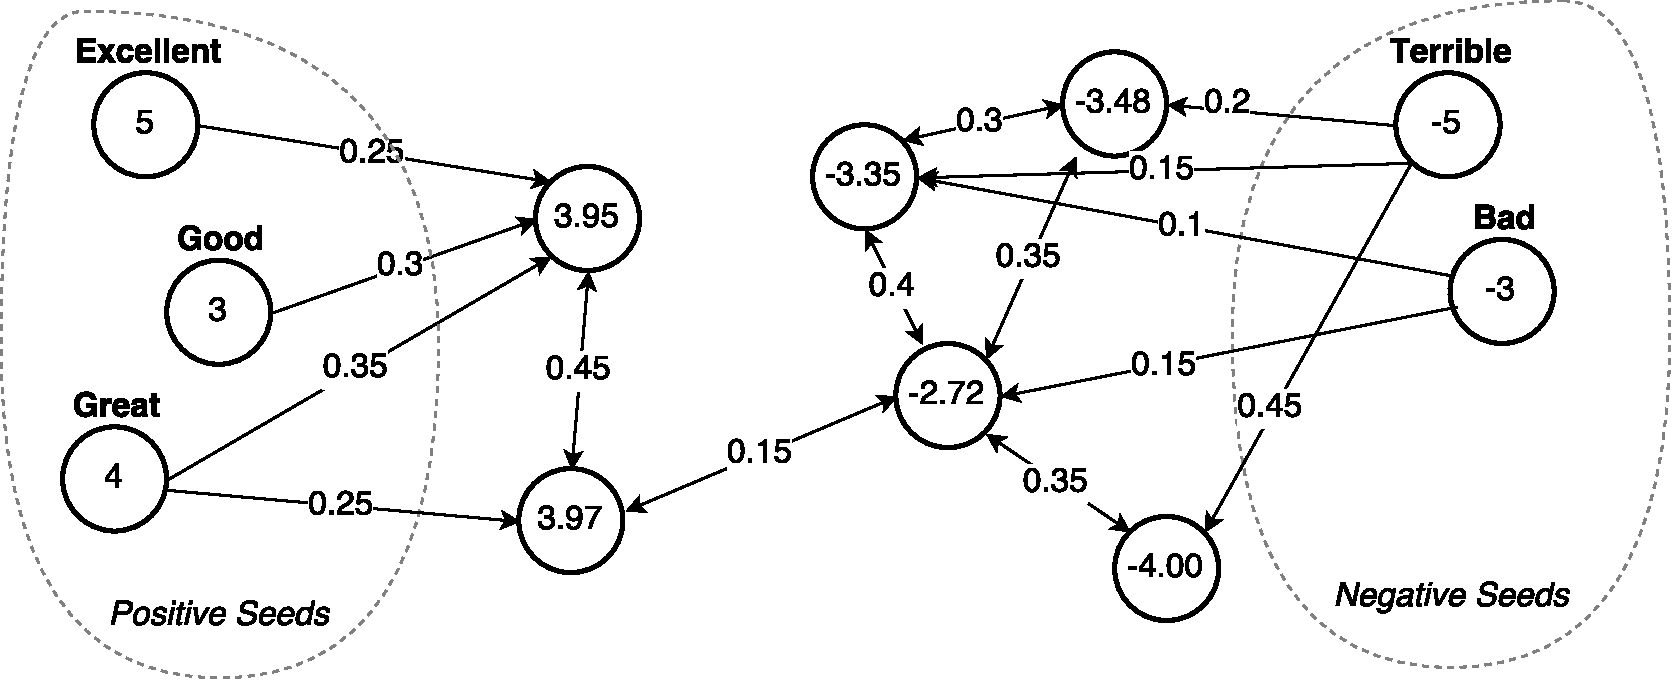
\includegraphics[width=\textwidth]{./figs/label_propagation}
        \caption{Using the Label Propagation Algorithm}
        \label{fig:label_propagation}
    \end{subfigure}
    \begin{subfigure}[b]{1.0\textwidth}
        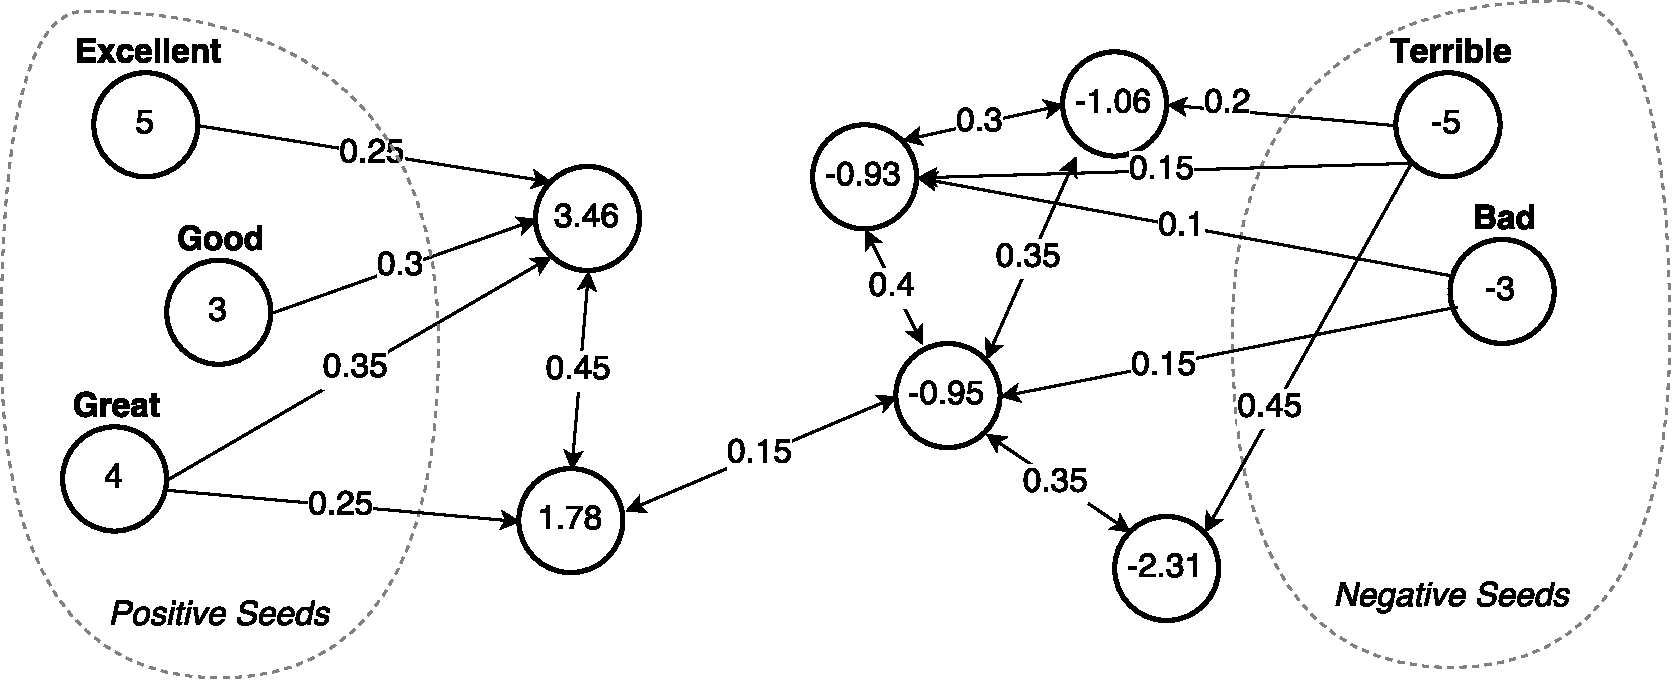
\includegraphics[width=\textwidth]{./figs/graph_propagation}
        \caption{Using the Graph Propagation Algorithm}
        \label{fig:graph_propagation}
    \end{subfigure}
    \caption{Comparison of propagation algorithms' end results}
    \label{fig:propagation_comparison}
\end{figure}


\subsection{Graph Propagation Algorithm}
\label{sec:graph_propagation_algorithm}
The Graph Propagation Algorithm is an alternate version of the LPA, specifically aimed towards sentiment lexicon creation based on graphs of lower quality, where not all edges are trustworthy. The algorithm was proposed by \cite{Velikovich2010}, arguing that the approach would alleviate the reinforcement effect of the LPA on lower quality graphs. Similarly to the LPA, an initial graph is created based on an appropriate relationship measure before all nodes representing the seed words are given an initial sentiment value. The nodes representing seed words are then traversed, propagating their sentiment value to all nodes within a distance $T$. On each step away from the seed node, the sentiment value is weighted using the edge weights between the nodes, representing their relational strength. The further away from the seed node a node is located, the lower the propagated sentiment value will be. Each node holds the max path from each seed node within a distance of $T$. After all seed nodes have propagated their sentiment value, the final sentiment value of each node is calculated by subtracting the sum of the max paths from negative seed nodes from the sum of max paths from positive seed nodes. The method is shown in Algorithm~\ref{alg:graph_propagation}. \\

\begin{algorithm}[t]
	\DontPrintSemicolon
    \caption{Graph Propagation Algorithm}
    \label{alg:graph_propagation}
    \KwIn{$G=(V,E)$, $w_{ij}\in[0,1]$, $\gamma \in \mathbb{R}$, $T\in \mathbb{N}$, $P$, $N$}
    \KwOut{Sentiment Lexicon, $pol \in \mathbb{R}^{|V|}$}
    
    $pol_i, pol_i^+, pol_i^- = 0$, $\forall i$\;
	$pol_i^+ = 1.0$, $\forall v_i \in P$\;
    $pol_i^- = 1.0$, $\forall v_i \in N$\;

	$a_{ii} = 1, a_{ij} = 0$, $\forall i \neq j$\;

	\For{$v_i \in P$}{
    	$F=\{v_i\}$\;
        \For{$t \gets 1$ \textbf{to} $T$}{
        	\For{$(v_k, v_j) \in E$ such that $v_k \in F$}{
            	$a_{ij} = \max \{a_{ij}, a_{ik} \cdot w_{kj}$\}\;
                $F=F \bigcup \{v_j\}$
        	}
        }
    }
    \For{$v_j \in V$}{
    	$pol_j^+ = \sum_{v_i \in P} a_{ij}$
    }

	Repeat steps 4-12 using $N$ to compute $pol^-$\;

	$\beta = \sum_i pol_i^+ / \sum_i pol_i^-$\;
	$pol_i = pol_i^+ - \beta pol_i^-$, $\forall i$\;
	\textbf{if} $|pol_i| < \gamma$ \textbf{then} $pol_i=0.0$, $\forall i$\;
\end{algorithm}

Figure~\ref{fig:graph_propagation} shows the result of running the Graph Propagation Algorithm on a small, dense graph. Notice how using LPA, a node received higher sentiment value having only one edge from positive seed words than a node having three edges from positive seed words, whereas using the Graph Propagation Algorithm, the more connected node received a much higher sentiment value than the single connected node.


\section{Classification Scoring Metrics}
\label{sec:classification_scoring_metrics}
To measure the performance of a classification system, a collection of scoring metrics are needed. In Sentiment Analysis the four scoring metrics precision, recall, F1--score and accuracy are often used. The calculation of these depends on values called \textit{true-positives}, \textit{false-positives}, \textit{true-negatives} and \textit{false-negatives}; $tp$, $fp$, $tn$ and $fn$ respectively. Here $tp$ and $tn$ are the number of examples correctly classified as positive and negative, while $fp$ and $fn$ are the number of examples falsely classified as positive and negative. This relationship can be viewed in the confusion matrix displayed in Table~\ref{tab:prediction_outcomes}.

\begin{table}[H]
    \centering
    \begin{tabular}{l|l|c|c|c}
        \multicolumn{2}{c}{}&\multicolumn{2}{c}{Predicted}&\\
        \cline{3-4}
        \multicolumn{2}{c|}{} & Positive & Negative\\
        \cline{2-4}
        \multirow{2}{*}{\rot{True}} & Positive & $tp$ & $fn$\\
        \cline{2-4}
        & Negative & $fp$ & $tn$\\
        \cline{2-4}
    \end{tabular}
    \caption{Confusion matrix for possible prediction outcomes}
    \label{tab:prediction_outcomes}   
\end{table}

\subsection*{Precision}
Precision is the ratio of the number of relevant returned results to the number of total returned results. The precision ratio describes how many of the returned results are relevant. Precision is defined as:
\begin{equation*}
    precision = \frac{tp}{tp+fp}
\end{equation*}

\subsection*{Recall}
Recall is the ratio of the number of relevant results to the number of overall relevant results. The recall ratio describes how many of the relevant results are returned.  Recall is defined as:
\begin{equation*}
    recall = \frac{tp}{tp+fn}
\end{equation*}

\subsection*{$F_{1}$-Score}
F-Score is the weighted combination of precision and recall, and in its general form defined as:
\begin{equation*}
    F_{\beta} = (1+\beta)\cdot\frac{precision\cdot recall}{(\beta ^2 \cdot precision) + recall}
\end{equation*}

The most commonly used $\beta$ value is $1$, this is known as $F_{1}$-score, which produces the harmonic mean of precision and recall. $F_{1}$-score is thus defined as:
\begin{equation*}
    F_{1} = 2\cdot\frac{precision\cdot recall}{precision + recall} = \frac{2tp}{2tp + fp + fn}
\end{equation*}

\subsection*{Accuracy}
Accuracy is the ratio of the number of true results to the number of total cases. The accuracy ratio describes how many of the results were accurately predicted as positive and negative. Accuracy is defined as:
\begin{equation*}
    accuracy = \frac{tp+tn}{tp+fp+tn+fn}
\end{equation*}


\section{Tools}
\label{sec:tools}

\subsection{Scikit-Learn}
\label{sec:background_scikit}
Scikit-Learn, by \cite{scikit-learn}, is a machine learning library, written in Python. It consists of implementations of a wide range of state-of-the-art machine learning algorithms built for both supervised and unsupervised medium-scale problems. It emphasises ease of use and good documentation, and plays an important role in this project. In the following paragraphs the most relevant concepts and features of Scikit-Learn are presented.

\subsection*{Transformer}
A \textit{Transformer} object in Scikit-Learn is used to extract or generate feature representations of the data. To extract different features, different transformers must be created.

\subsection*{Pipeline}
Scikit-Learn provides a \textit{Pipeline} object, allowing pipelining of machine learning processes. The pipeline makes it easy to perform and chain processes such as preprocessing and feature extraction together with a machine learning algorithm in a sequential and tidy manner. In other words, it allows sequential and parallel application of a list of estimators. An estimator is in this context either an object that is able to learn from data, such as a classifier, or a \textit{Transformer} object that extracts features from raw data.

\subsection*{Feature Union}
A \textit{Feature Union} is an object included in the \textit{Pipeline} framework and is a useful tool in feature extraction. The standard \textit{Pipeline} chains transformers together in a sequential manner where data from one \textit{Transformer} is fed directly into the next \textit{Transformer}. A \textit{Feature Union} on the other hand allows for a collection of transformers to be fed the exact same input data. This is especially useful when wanting to extract a series of different features from the same data. The resulting feature vectors from the \textit{Transformer}s in the \textit{Feature Union} are concatenated into a final feature matrix. 

\subsection*{Grid Search}
The \textit{Pipeline} framework allows performing a \textit{Grid Search} across all \textit{Transformer} or estimator parameters. The \textit{Grid Search} takes a set of possible values for each parameter in each transformer and searches through all possible parameter combinations, looking for the combination that yields the best performance overall.

\subsection{GATE TwitieTagger}
The GATE TwitieTagger, by \cite{twitieTagger}, is a \acf{pos} tagger specifically created for tweets. As described in Section~\ref{sec:background_nlp}, the \ac{pos} tagger takes as input a sentence and returns the same sentence where each word is replaced by its \ac{pos} tag. \\

Another powerful \ac{pos} tagger tailored for tweets is the TweeboParser by \cite{Gimpel11}. TweeboParser is very complex and is written in several programming languages linked together with Shell and Python scripts. Because of this, we decided to use the much simpler GATE TwitieTagger which is only written in Java. In terms of performance, both report a similarly high token accuracy values: 91\% and 90\% for GATE TwitieTagger and TweeboParser, respectively.

\subsection{VADER Sentiment Analysis}
\label{sec:vaderSentiment}
VADER (Valence Aware Dictionary and sEntiment Reasoner), by \cite{vaderSentiment}, is a lexicon based sentiment analysis tool specifically tuned towards social media. VADER goes beyond the simple bag-of-words model and takes into consideration word order and degree modifiers.

\subsection{Emoji-Java}
Emoji-Java\footnote{Emoji-Java: \url{https://github.com/vdurmont/emoji-java}} is a lightweight library that lets you convert from Unicode emoji characters to their alphabetical, decimal and hexadecimal representations. The alphabetical representation, called alias, is a single word describing emote; for example, {\DejaSans ☺} is translated into "smile".


\section{Datasets}
\label{sec:datasets}
In this section all external datasets used is described. In addition we downloaded a large Twitter dataset using the Tweet Streaming API to create our sentiment lexicon. That dataset is described in detail in Section~\ref{sec:twitter_streaming_dataset}.

\subsection{TweetNLP --- Twitter Word Cluster}
\label{sec:tweetnlp}
TweetNLP is a set of tools made specifically for Twitter \ac{nlp} tasks. A part of TweetNLP is a hierarchical Twitter word cluster, by \cite{Owoputi12}, that was generated using Brown clustering, based on 56 million unique tweets. We have incorporated this clustering as a simple dictionary from word to cluster ID. 

\subsection{SemEval 2016 Twitter Sentiment Dataset}
As part of the \ac{semeval} 2016 five datasets have been made available. These comprise a training set and a test set from \ac{semeval} 2013, and test sets from \ac{semeval} 2014, 2015 and 2016. We used the 2013 training sets for training, while the test sets were only used to test our system. To access the datasets, they all had to be downloaded through the Twitter API. Portions of the tweets have been deleted since the datasets were originally created and are therefore no longer available. Table~\ref{tab:dataset_overview} gives an overview of the datasets used, comparing the sizes of the original annotated datasets to the sizes and class distributions of the datasets actually available at the time they were downloaded.

\makeatletter
    \setlength\@fptop{0\p@}
\makeatother

\begin{table}[htbp]
    \begin{tabular}{| l | l | l | l | l | l |}
        \hline
         & \multicolumn{2}{c|}{\textbf{Size}} & \multicolumn{3}{c|}{\textbf{Class distribution}} \\ \hline
        \textbf{Name} & \textbf{Original} & \textbf{Downloaded} & \textbf{Positive} & \textbf{Neutral} & \textbf{Negative} \\ \hline
        2013-train & 9684 & 8748 & 3283 & 4175 & 1290 \\ \hline
        2013-test & 3813 & 3087 & 1258 & 1367 & 462 \\ \hline
        2014-test & 1853 & 1509 & 794 & 564 & 151 \\ \hline
        2015-test & ? & 2390 & 1038 & 987 & 365 \\ \hline
        2016-test & ? & 20632 & 7059 & 10342 & 3231 \\ \hline
    \end{tabular}
    \caption{Overview of SemEval datasets used in the project}
    \label{tab:dataset_overview}
\end{table}

\glsresetall

%!TEX root = ../report.tex
\chapter{Related Work}
\label{cha:related_work}
In this chapter, an overview of the state-of-the-art within \ac{tsa} is presented, before common approaches within lexicon based \ac{sa} systems and automatic creation of sentiment lexica are described in more detail. The overview of the state-of-the-art within \ac{tsa} will act as an introduction to \ac{tsa}, introducing central aspects and concepts within the field, whereas the in-depth descriptions of the common approaches within lexicon based \ac{sa} and automatic creation of sentiment lexica forms the basis for the systems developed in the thesis. In addition the highly relevant \ac{semeval} is described, being at the forefront of research within the field of \ac{tsa}.

\section{Literature Review Method}
\label{sec:literature_review_method}
Based on the goals presented in Section~\ref{sec:project_goals}, there were three main areas we wanted to research: state-of-the-art \ac{tsa}, lexicon based \ac{sa} and automatic creation of sentiment lexicon.\\

The research conducted when constructing the state-of-the-art within \ac{tsa} was mainly based on the top performing \ac{tsa} systems participating in \ac{semeval}, over the last few years. The reason for focusing primarily on \ac{tsa} systems participating in \ac{semeval} is that it is the main arena for \ac{tsa} systems, with new and better systems developed each year. \\  

Regarding the fields of lexicon based \ac{sa} and automatic creation of sentiment lexicon, which are the main focus areas of the thesis, an in depth literature review was conducted. First a series of candidate papers were collected within both fields using the search engine Google Scholar. After all candidate papers had been collected, each paper was reviewed and scored based on the relevance towards the specific field. The papers we found most relevant were then used to identify the most common approaches within each of the two fields.


\section{The International Workshop on Semantic Evaluation}
\label{sec:SemEval}
The \acf{semeval} is a workshop where several computational semantic language analysis systems are developed to solve a series of shared tasks. The overall process of the workshop consists of three steps: receive relevant training data, develop the system and evaluate the system. In recent years the workshop has been hosted annually, where some of the shared tasks have carried over from one year to the next. Among these is a collection of tasks centered around \ac{tsa}. As being a part of \ac{semeval} each year since 2013, the \ac{tsa} tasks have yielded significant improvements to the state-of-the-art in the field, as will be discussed in the following section.    

\section{State-of-the-Art in Sentiment Analysis}
\label{sec:state_of_the_art}
Based on the development in recent years within \ac{tsa}, a typical approach has been identified. The approach uses a supervised machine learning system, consisting of three main steps: preprocessing, feature extraction and classification. Preprocessing is used in order to remove noise and standardize the tweet format, by for example replacing or removing URLs. Desired features of the tweets are then extracted, such as sentiment scores using specific sentiment lexica or the occurrence of different emoticons. Finally, a classification is performed using the extracted features.

\subsection{Preprocessing}
The preprocessing of tweets in \ac{sa} commonly consists of a series of tasks in order to normalize the tweet format and prepare it for feature extraction. The main tasks in preprocessing commonly revolve around text filtering and negation detection. 

\subsection*{Text Filtering}
\label{sec:text_filtering}
Text filtering often includes removing items providing minimal information regarding the actual classification task. Items such as user mentions and URLs are therefore often substituted with tags as done by \cite{GoSentimentAnalysis09}, where the tag ``USER'' is used for user mentions and the tag ``URL'' for URLs. Another common approach is to remove the URLs and user mentions completely.\\

The use of retweets\footnote{Until early 2015 retweeting was not an official Twitter feature and users used to tweet with `RT' at the beginning of a tweet to indicate that the tweet was a re-post of someone else's content.} is also often handled as a text filtering task during preprocessing. The retweets are detected by the tag `RT', which indicates that the following segment of the tweet is a repost of someone else's tweet. This is commonly handled by simply removing the retweet tag `RT' from the tweet, because the `RT' tag by itself carries no information. A retweet can be about how someone agrees or disagrees about the original quote and analysis of the text itself is needed to determine which one it is. \\

Elongated words are common in tweets. Elongated words are words spelled with extra characters, such as ``booooring'' or ``coool''. These words are often modified by reducing the surplus of equal consecutive characters. The words are then either reduced down to the actual correct spelling of the word, ``booooring'' becomes ``boring'', or down to a maximum number of consecutive equal characters. With a maximum of 2 consecutive equal characters, ``booooring'' becomes ``booring''. The reduction is done to be able to group various elongations of the same word under one entry, the aggregated approach helps determine the overall sentiment more accurately. A reason for not removing all of the extra characters is that elongation can be a form of expressing the sentiment, and can therefore be useful in the analysis. \\


\subsection*{Negation Detection}
Detecting negation (Section~\ref{sec:background_nlp}) in tweets has become an integral part of most \ac{tsa} systems. This is commonly done by looking for negation cues such as \textit{"not"}, \textit{"wouldn't"} and \textit{"ain't"} in the tweets, before determining the potential scope of the negation. To determine the scope, the collection of words affected by the negation cue, a simple method proposed by \cite{Das01yahoo} is often used. The simple approach consists of selecting the $n$ consecutive words appearing after the negation cue, and marking them as negated. Another common approach is to mark all consecutive words appearing after the negation cue until reaching the next punctuation mark as negated. As to how much each individual word is affected, there are two main approaches. The first approach being simply reversing the sentiment value of the word, and the other being a slight adjustment of the sentiment value of the word towards the opposite polarity. Using the second approach, the unigram \textit{"great"} with a sentiment value of 3 should in a negated context get a less positive value of, for instance, 0.5. A word with low positive initial sentiment value should with this approach end up with a negative sentiment value.


\subsection{Feature Extraction}
In order to predict or say anything about the overall sentiment of a tweet, the features of the tweet need to be identified and evaluated. This process is commonly called feature extraction. In our review of the participating \ac{tsa} systems in \ac{semeval} (2013-2015), a state-of-the-art feature set has been identified. The state-of-the-art feature set consist of the features most commonly used by the top ranked systems, first introduced by \cite{MohammadKZ2013} in \ac{semeval}-2013. The state-of-the-art feature set includes the following features:

\begin{itemize}
    \item \textit{Word $n$-grams}: Collecting and weighting of words or collections of consecutive words.
    \item \textit{Char $n$-grams}: Collecting and weighting of characters or collections of consecutive characters.
    \item \textit{Word clusters}: Determining which cluster each word in a tweet belongs to. 
    \item \textit{Prior Polarity Sentiment Lexica}: Collecting the sentiment value of the individual words in a tweet, by looking up the words in specialized prior polarity sentiment lexica, and extracting features based on the values.
    \item \textit{Part-of-Speech tagging}: Utilizing specialized Twitter Part-of-Speech taggers to tag each word and count the occurrences of each tag.
    \item \textit{Punctuation}: The number of consecutive punctuation marks and whether the last character of a tweet is an exclamation mark or a question mark.
    \item \textit{Emoticons}: The number of positive and negative emoticons.
    \item \textit{Negation}: The marked negation scopes are utilized using prior polarity lexica able to handle words in negated contexts. The negation marking also has an effect in \textit{Word $n$-grams}, \textit{Char $n$-grams} and Prior Polarity Sentiment Lexica.
\end{itemize}


\subsection{Classification}
By using the feature representation of tweets, created in the feature extraction step, a supervised machine learning algorithm called a classifier is commonly used to perform the classification task. Among the supervised machine learning algorithms, the most popular within \ac{tsa} are \ac{svm}, Logistic Regression, Stochastic Gradient Descent and Naïve Bayes. In Table~\ref{tab:semeval_2015_results} the top ten submissions of \ac{semeval}-2015 are listed together with the machine learning algorithm used. We see that the \ac{svm} is the most used algorithm, which by \cite{Svetlana14} is considered to be the state-of-the-art algorithm within \ac{tsa}. \\     

\noindent\begin{table}[ht]
    \begin{tabular}{| l | l | l |}
        \hline
        \textbf{Rank} & \textbf{Name} & \textbf{Classifier} \\ \hline
        1 & Webis & Ensemble of four classifiers, averaging results \\ \hline
        2 & unitn & Deep Convolutional neural network (CNN) \\ \hline
        3 & lsislif & Logistic regression \\ \hline
        4 & INESC-ID & Stochastic Gradient Descent \\ \hline
        5 & Splusplus & Two stage classifier. SVM and CNN \\ \hline
        6 & wxiaoac & SVM \\ \hline
        7 & IOA & SVM with RBF kernel \\ \hline
        8 & Swiss-Chocolate & SVM, Logistic regression and random forest \\ \hline
        9 & CLaC-SentiPipe & Linear SVM and Logistic regression \\ \hline
        10 & TwitterHawk & Linear SVM \\ \hline
    \end{tabular}
    \caption{Overview of top 10 submissions for SemEval 2015}
    \label{tab:semeval_2015_results}
\end{table}

\subsection*{One-Step vs. Two-Step Classification}
The most common classification approach in \ac{tsa} is a one-step process, where a single machine learning algorithm classifies the tweets into three different classes; positive, negative and neutral. Most of the top ranked submissions in \ac{semeval}-2014 and \ac{semeval}-2015 used this approach. \\

There are, however, other approaches. One of these is the two-step classification approach, consisting of two consecutive steps: subjectivity classification and polarity classification. In the subjectivity classification step, tweets will either be classified as subjective or objective/neutral. The tweets classified as subjective will then proceed to the polarity classifier, where they are classified as either positive or negative. \\

In \ac{semeval} 2015, the top ranked TSA system by \cite{Webis15} used yet an other approach, by utilizing an ensemble of four classifiers. In the ensemble approach, classification is commonly done through a vote among the classifiers, where each classifier votes for the class it has predicted. \citeauthor{Webis15} let each classifier present its calculated probability for each class, and the class with highest average probability is chosen.  


\section{Automatic Creation of Sentiment Lexica}
\label{sec:automatic_generation_of_sentiment_lexica}
Manual annotation of large amounts of data is costly. This also applies to the task of annotating sentiment lexica, where each $n$-gram in a large collection of $n$-grams should be assigned a sentiment value. Not only should the annotator decide whether or not the $n$-gram is positive or negative, but also the sentimental strength of the $n$-gram. For example, the unigram \textit{"great"} should get a positive sentiment score that is higher than the unigram \textit{"good"}, because \textit{"great"} is more positive. To overcome these hurdles, a lot of research has been done within the field of automatic creation of sentiment lexica, where $n$-grams should both be collected and annotated automatically. As a result of the research, a series of different approaches has been proposed on the subject over the past 20 years. 


\subsection{Collecting data}
Before beginning the annotation process, the $n$-grams to include in the lexicon should be collected. The most common approach is to extract these from a large corpus of text documents capturing the language features the lexicon is aimed at. For example, a lexicon aimed at user reviews should probably use a large corpus of user reviews, while a lexicon aimed at tweets should probably use a large corpus of tweets. Candidate entries are commonly selected based on a frequency analysis over the complete corpus where the most frequent $n$-grams are selected. \cite{MohammadKZ2013} selected all unigrams and bigrams as candidate entries, while \cite{Velikovich2010} selected all $n$-grams up to length 10 before filtering out $n$-grams based on their frequency and mutual information. In the latter approach, only the $n$-grams are kept where the co-occurrence of the included words forms common phrases or sayings. At this stage, stopwords are often filtered out using a predefined list of stopwords. That is, the most common words in a language, e.g., \textit{the, is, at} and \textit{a} are removed. These words will appear frequently in both positive and negative contexts and should therefore on their own not be given a sentiment value.


\subsection{Annotating candidate \textit{n}-grams}
The common methods for annotating the selected candidate $n$-grams can be divided into two main types. One, where the documents from which the candidate $n$-grams were selected are labeled, and another where the documents are unlabeled. Labeled documents can for instance be reviews or tweets that are labeled as positive or negative.


\subsection*{Annotating using labeled documents}
When using a corpus of labeled documents to annotate candidate $n$-grams, the association measure \ac{pmi} is commonly used. The \ac{pmi} value for $n$-grams in a positive context and in a negative context are calculated separately and the final sentiment score of an $n$-gram is calculated by subtracting the \ac{pmi} for the $n$-gram in a negative context from the \ac{pmi} in a positive context, as described in Section~\ref{sec:pmi_lexicon}. Using the aforementioned method and two different Twitter corpora, \cite{MohammadKZ2013} created the \textit{Sentiment140} and \textit{HashtagSentiment} lexica. The labeled tweets used to create the two were collected using seed sets of positive and negative emoticons and hashtags. If a tweet contained a positive emoticon or hashtag the tweet was labeled as positive, and if a tweet contained a negative emoticon or hashtag it was labeled as negative. Both the \textit{Sentiment140} lexicon and the \textit{HashtagSentiment} lexicon are often used as lexica in the sentiment lexicon feature in machine learning \ac{tsa} systems. Examples of this are the winning \ac{tsa} system of Task 10 subtask B in \ac{semeval} 2015, \cite{Webis15}, and the fifth best system competing on the same task by \cite{Splusplus15}.


\subsection*{Annotating using unlabeled documents}
The \ac{pmi} measure can also be used when annotating using a corpus of unlabeled documents. \cite{turneylittman2002} proposed a method where a seed set containing positive and negative words based on opposing pairs, e.g. \textit{good/bad, excellent/poor} was used. Each candidate word got its sentiment value by subtracting the \ac{pmi} for negative context from the \ac{pmi} for positive context. A candidate word is in a negative context if one of the negative seed words is within a window of 10 words to the left or to the right of the candidate word. The same applies to the positive context. \\

Another approach using unlabeled documents is the graph approach. For the graph approach two different variants have been proposed. For both variants the similarity between all candidate $n$-grams, and between the candidate $n$-grams and a seed set of positive and negative words are calculated before each $n$-gram is initialized as a node in a graph. The edges between the nodes are weighted according to the similarity between them. If the similarity is below a set threshold, the edge will not be created. Similarity can be calculated in a number of different ways: \cite{Velikovich2010} determined the edge weights by calculating the cosine similarity between constructed context vectors of the $n$-grams, while \cite{Zhu02learningfrom} sat the edge weights to be the Euclidean distance between the $n$-grams.\\  

In the graph propagation variant, described in Section~\ref{sec:graph_propagation_algorithm}, proposed by \cite{Velikovich2010}, the nodes representing the seed set should be initialized with a sentiment score according to its orientation (negative or positive), before propagating their sentiment value to the nodes laying on a path of length $k$ away from them. The sentiment value of an $n$-gram is then calculated by adding the sum of negative sentiment scores to the sum of positive sentiment scores that has been propagated to the node representing the $n$-gram.\\ 

The second variant proposed by \cite{Zhu02learningfrom}, the label propagation approach, is quite similar to the graph propagation approach outlined above. The main difference between the two is how the sentiment values are calculated. Where the graph propagation variant calculates the sentiment value to be the sum of the max paths from seed words to a given $n$-gram, the label propagation variant calculates the sentiment value as the weighted average of the $n$-grams neighbors. Whereas each node in the graph propagation variant only holds the max path from a seed word, the nodes in the label propagation variant can possibly hold multiple paths to a specific seed word.\\   

\citeauthor{Velikovich2010} argued that with a high quality graph where each path is trustworthy the label propagation variant will work as intended. Words close to a positive seed word, for instance, will get a higher score than words further away. However, with a lower quality graph, which often may the case with Twitter data, what is called the reinforcement effect described in Section~\ref{sec:label_propagation_algorithm}, may occur, resulting in undesired behavior.


\section{Lexicon Based Sentiment Analysis}
\label{sec:lexion_based_sentiment_analysis}
Lexicon based \ac{sa} is the task of performing \ac{sa} solely based on one or multiple sentiment lexica. The overall performance of a lexicon based \ac{sa} system is therefore closely related to the quality of the sentiment lexicon used, but also how the sentiment lexicon information is used. In recent years, most \ac{sa} systems use a machine learning approach, with sentiment lexica as a feature among a series of other features. The number of new lexicon based \ac{sa} systems that have appeared in recent years is therefore few. Although the task of classification differs between a lexicon based \ac{sa} system and a machine learning \ac{sa} system, the sentiment lexica features in machine learning systems are based around the same ideas used by lexicon based \ac{sa} systems. The common approach consists of two main steps: sentence analysis and sentiment calculation.


\subsection{Sentence Analysis}
Before the $n$-grams in a sentence are looked up in a sentiment lexicon and given a sentiment value, the sentence itself is analysed in search of specific features. These features are used to adjust the raw sentiment values collected from the sentiment lexica.


\subsection*{Negation} 
Similarly to the machine learning approaches to \ac{sa}, the detection of negation is also an important feature in lexicon based \ac{sa}, using the approaches described in Section~\ref{sec:state_of_the_art}.


\subsection*{Intensification}
In systems such as by \cite{vaderSentiment} and \cite{Taboada2011}, intensifiers are used in the classification process. In addition to detecting negation, words working as intensifiers or degree adverbs are detected. Degree adverbs are words such as \textit{"very"}, \textit{"completely"} and \textit{"hardly"}, and affect the following word by either boosting or dampening its sentiment value. The main idea is that in the sentence \textit{"that was good"}, for instance, the word \textit{"good"} should get a lower sentiment value than in the sentence \textit{"that was very good"}, because of the booster word \textit{"very"}. While in the sentence \textit{"that was kind of good"}, on the other hand, the word \textit{"good"} should get a lower sentiment value because of the dampener \textit{"kind of"}. There are two common approaches to how the intensifiers should affect the following word. \cite{Polanyi06} used a \textit{fixed intensification} method, where a fixed amount is added to or subtracted from the sentiment value of the affected word. \cite{Taboada2011} on the other hand used a \textit{percentage intensification} method, where the sentiment values of the affected words are multiplied by a value $x>1$ for boosters and $0<x<1$ for dampeners.  


\subsection{Sentiment Calculation}
The common approach to calculate the final sentiment value of a sentence is to sum up the sentiment values of each $n$-gram in the sentence. Depending on whether or not negation and intensification were detected during the analysis step, the sentiment values of the affected $n$-grams are adjusted accordingly. In order to classify the sentence based on its final sentiment value, thresholds for positive and negative sentiment scores must be decided upon. With a final sentiment value above the threshold for positive sentences, the sentence is classified as positive. If the value is below the threshold for negative sentences, the sentence is classified as negative. With a final sentiment value between the two thresholds the sentence is classified as neutral. 

\glsresetall

\include{sections/annotation}
%!TEX root = ../report.tex
\chapter{Initial Experiment}
\label{ch:initial_experiment}
In the fall of 2015, we developed a state-of-the-art \ac{tsa} system based on the most common approaches within the field, outlined in Section~\ref{sec:state_of_the_art}. The system was created for the \ac{semeval} 2016 and its \ac{tsa} specific task: "Message Polarity Classification".\footnote{SemEval 2016 Task 4a, Message Polarity Classification: Given a tweet, predict whether the tweet is of positive, negative, or neutral sentiment.} The development of the system acted as both an introduction to the field of \ac{tsa} and as inspiration for the project goals listed in Section~\ref{sec:project_goals}. In this chapter the overall system architecture is described, followed by test results and results from our participation in \ac{semeval} 2016. Shorter versions of this system description previously appeared in \cite{JahFre16} and \cite{JahFre15}.

\section{Sentiment Classifier Architecture}
To solve the three-class classification problem, a general multi-class classifier, named \textit{BaseClassifier}, was created. By following a general interface, several \textit{BaseClassifier}s could be combined sequentially to create a multi-step classifier, or in parallel to create an ensemble classifier.


\section{BaseClassifier}
\label{sec:core_architecture}
The Sentiment Analysis system created was developed using the Python programming language and the Scikit-Learn machine learning framework described in Section~\ref{sec:background_scikit}. The \textit{BaseClassifier} consists of a three step process: preprocessing, feature extraction, and classification or training. The three consecutive steps are handled by the \textit{Pipeline} also described in Section~\ref{sec:background_scikit}. Each \textit{Transformer} (feature extractor) is presented with preprocessed data. The preprocessing methods used are dependent on the different \textit{Transformer}s and the features they aim to extract. The different \textit{Transformer}s and the range of preprocessors used are described later in this section. Figure~\ref{fig:core_architecture} illustrates the overall architecture of the system. \\

\begin{figure}[t]
    \begin{center}
        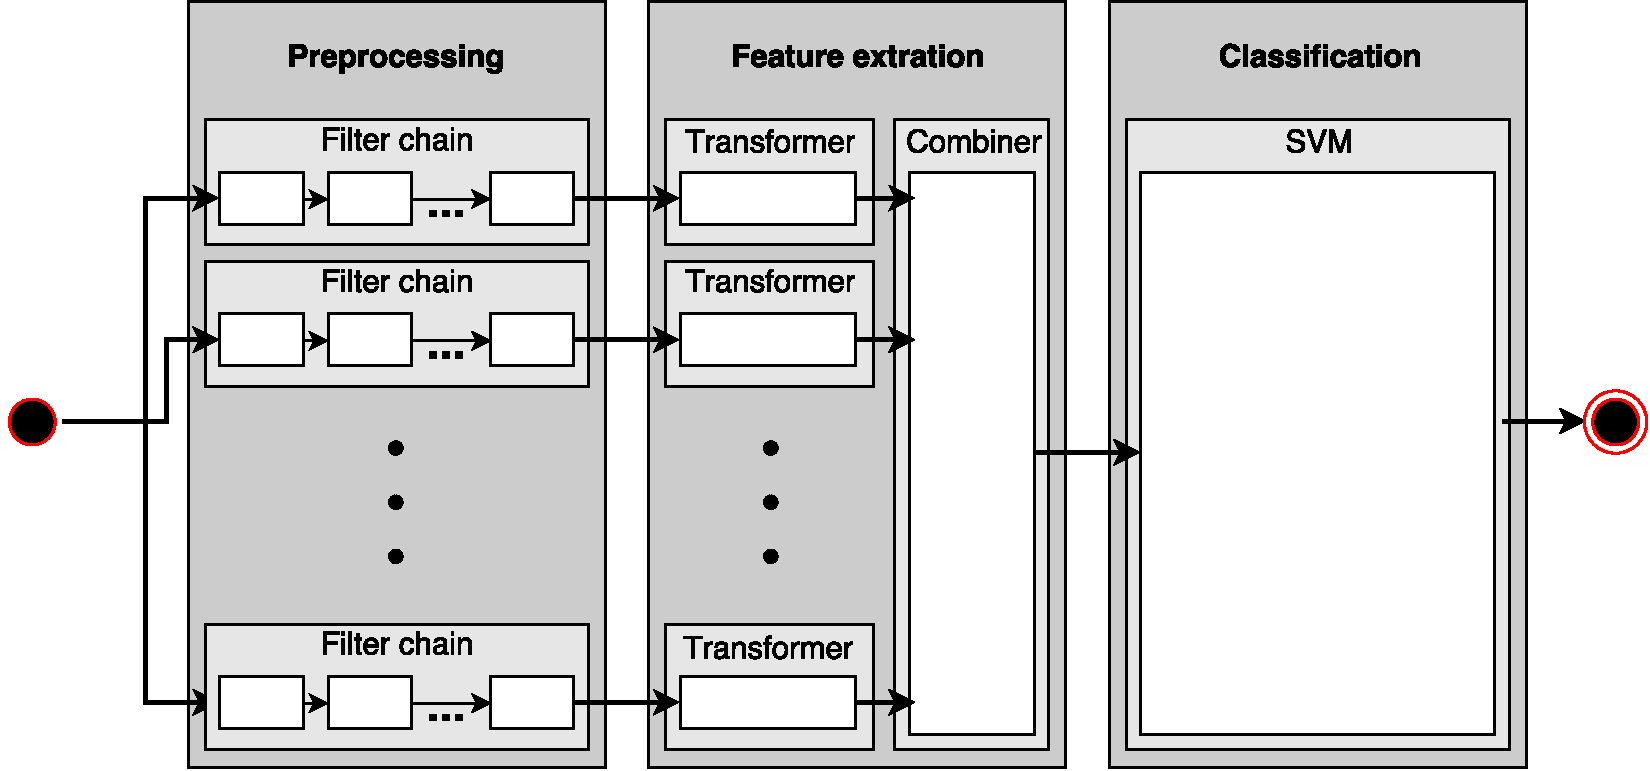
\includegraphics[width=\textwidth]{./figs/core_architecture}
    \end{center}
    \caption{Architecture of the Initial Experiment}
    \label{fig:core_architecture}
\end{figure}

The \textit{BaseClassifier} is very general. When creating a \textit{BaseClassifier} instance, it takes in a dictionary that specifies all of its parameters. The parameter dictionary includes the classifier algorithm, such as SVM, Naïve Bayes or MaxEnt, options for each of the transformers, for example $n$ value for the character and word $n$-gram transformers, or which preprocessing functions to use.

\subsection{Preprocessing}
The preprocessing step of the system modifies the raw tweets before they are passed to feature extraction, and is a necessary stage to improve the overall performance of the system. In this stage simple methods are chained together to modify raw tweets using regular expressions. Limiting each preprocessor to perform only one simple task allows for easy management of the preprocessing used by the different transformers. Table~\ref{tab:filters} lists all the basic preprocessors.

\begin{table}[t]
    \centering
    \begin{tabular}{| l | p{9.3cm} |}
        \hline
        \textbf{Filter} & \textbf{Description} \\ \hline
        %html_decode
        tokenize & Performs tweet tokenization using tokenizer by \cite{PottsTokenizer} \\ \hline
        lower\_case & Transforms all uppercase characters to lowercase \\ \hline
        no\_emotes & Replaces various emoticons with empty string \\ \hline
        no\_user & Replaces all username mentions with empty string \\ \hline
        no\_rt\_tag & Replaces all RT tags with empty string \\ \hline
        no\_url & Replaces all URLs with empty string \\ \hline
        no\_hashsign & Replaces all hash marks (\#) with empty string \\ \hline
        no\_hashtag & Replaces all hash marks along with the following tag with empty string \\ \hline
        limit\_chars & Removes all non alphabetic or space characters \\ \hline
        limit\_repeat & Limits maximum repeating of a single character to three \\ \hline
    \end{tabular}
    \caption{List of preprocessors used in the Initial Experiment}
    \label{tab:filters}
\end{table}

\subsection*{Negation Detection}
A subset of the transformers perform better when negation is identified in the tweets. Negation detection is therefore an important tweet preprocessing step performed on all tweets before being sent to negation-dependent transformers. \\

To perform negation detection, the system uses a simple approach, where $n$ words appearing after a negation cue are marked as negated by attaching ``\texttt{\_NEG}'' to the end of each word. If a punctuation mark is encountered before reaching the $n$--th word, the negation marking is stopped. By setting $n=-1$, negation marking is extended until the next punctuation or the end of the tweet. To detect the negation cues, all words in a tweet are checked against a list of negation cues. All negation cues used in our system are listed in Table~\ref{tab:negation_cues}. The negation cues were adopted from \cite{Councill10}, additionally we added common misspellings and other closely related words by looking up each negation cue in TweetNLP's word cluster, described in Section~\ref{sec:tweetnlp}.

\begin{table}[t]
    \centering
    \begin{tabular}{| l | l | l | l | l | l | l |}
        \hline
        \multicolumn{7}{|c|}{\textbf{Negation Cues}} \\ \hline
        ain't & aint & anit & can't & cannot & cant & couldn't \\ \hline
        couldnt & didn't & didnt & dnt & does'nt & doesn't & doesnt \\ \hline
        don't & dont & hadn't & hasn't & hasnt & haven't & havent \\ \hline
        havn't & havnt & isn't & isnt & lack & lacking & lacks \\ \hline
        no & nor & not & shouldn't & shouldnt & wasn't & wasnt\\ \hline
        won't & wont & wouldn't & wouldnt & \multicolumn{3}{c|}{} \\ \hline
    \end{tabular}
    \caption{List of negation cues used in the Initial Experiment}
    \label{tab:negation_cues}
\end{table}


\subsection{Feature Extraction}
\label{sec:feature_extraction}
In our system the feature extraction set is implemented as a Scikit-Learn \textit{Feature Union}, which is a collection of independent transformers (feature extractors), that builds a feature matrix for the classifier. Each feature we want to extract is represented by a \textit{Transformer}. Table~\ref{tab:feature_extractors} gives an overview of all the feature extractors used in the system.

\begin{table}[ht]
    \centering
    \begin{tabular}{| l | p{10cm} |}
        \hline
        \textbf{Features} & \textbf{Description} \\ \hline
        Word $n$-grams & Extracts TF--IDF values for combination of sequential words as described in Section~\ref{sec:background_tfidf} \\ \hline
        Char $n$-grams & Extracts TF--IDF values for combination of sequential characters \\ \hline
        Lexicon & Extracts a few values that are calculated as a function of the sentiment value of words in the tweet \\ \hline
        Word Clusters & Extracts a \textit{Bag-of-Words} model of cluster IDs for each token in the tweet \\ \hline
        Part-of-Speech & Extracts a \textit{Bag-of-Words} model of part-of-speech tags for each token in the tweet \\ \hline
        Emoticons & Extracts number of positive and negative emoticons found in the tweet \\ \hline
        Punctuation & Extracts number of repeated alphabetical and grammatical signs \\ \hline
        VADER & Extracts results from VADER sentiment analysis \\ \hline
    \end{tabular}
    \caption{List of feature extractors used in the Initial Experiment}
    \label{tab:feature_extractors}
\end{table}


\subsection*{TF--IDF Transformer}
Both \textit{Word n-grams} and \textit{Character n-grams} are realized using a \ac{tfidf} vectorizer that uses the bag of words model outlined in Section~\ref{sec:background_nlp}. Our implementation extends Scikit-Learn's default \textit{TfidfVectorizer}.


\subsection*{Lexicon Transformer}
The sentiment lexicon feature is represented by a single transformer using multiple different prior polarity sentiment lexica. The lexica used are a combination of automatic and manually annotated lexica, where some also contain sentiment scores for words in negated contexts. \\

The automatically annotated lexica used are the \textit{Sentiment140} and the \textit{HashtagSentiment} by \cite{MohammadKZ2013}, and contain sentiment scores for both unigrams and bigrams, where some are in a negated context. The unigrams and bigrams in a negated context are listed with a ``\texttt{\_NEG}'' attachment to differentiate between the two types of sentiment scores. \\

The features extracted for each tweet from these two lexica are adopted from \cite{MohammadKZ2013} and comprise:
\begin{itemize}
    \item The number of unigrams or bigrams with sentiment score $\neq0$.
    \item The sum of all sentiment scores.
    \item The highest sentiment score.
    \item The sentiment score of the last unigram or bigram.
\end{itemize}

The manually annotated lexica we used are the \textit{MPQA} by \cite{Wilson05}, the \textit{BingLiu} by \cite{Hu04}, the \textit{AFINN} by \cite{AFINN}, and the \textit{NRC Emoticon} lexicon by \cite{MohammadKZ2013}. The \textit{MPQA} and the \textit{BingLiu} lexica do not list sentiment scores for words, but instead whether a word contains positive or negative sentiment. After checking a word of a tweet against these lexica, the word is either given the score $-1$ or $+1$, for a negative or positive word sentiment, respectively. The \textit{AFINN} and the \textit{NRC Emoticon} lexica are similar to the two automatically annotated lexica described above, where each word for the \textit{AFINN} lexicon and each emoticon for the \textit{NRC Emoticon} lexicon is given a sentiment score. \\

Also for the manually annotated lexica, four features were extracted. The four features are as above, adopted from \cite{MohammadKZ2013} and comprise:
\begin{itemize}
    \item The sum of positive scores for words not in a negated context.
    \item The sum of negative scores for words not in a negated context.
    \item The sum of positive scores for words in a negated context.
    \item The sum of negative scores for words in a negated context.
\end{itemize}


\subsection*{Word Cluster Transformer}
The word cluster transformer extracts the word cluster feature by counting the occurrences of the different cluster IDs in each tweet. That is, if a word in a tweet exists in a cluster, a counter for that specific cluster ID is incremented by one. The word cluster used is described in Section~\ref{sec:tweetnlp}.

\subsection*{Part-of-Speech Transformer}
Uses the GATE TwitieTagger to assign part-of-speech tags to every token in the text, the tag occurrences are then counted and returned.

\subsection*{Punctuation Transformer}
The occurrences of continuous use of punctuation marks and characters are detected by the punctuation transformer. The feature it extracts is the number of these occurrences. 

\subsection*{Emoticon Transformer}
Similarly to the punctuation transformer, the emoticon transformer also searches for specific occurrences of characters that make up an emoticon in a tweet. For the emoticon transformer this is the use of happy and sad emoticons. The features it extracts are therefore the number of happy emoticons and the number of sad emoticons.

\subsection*{VADER Transformer}
The VADER transformer is very simple, it simply runs the VADER sentiment analysis tool, described in Section~\ref{sec:vaderSentiment}, and extracts the output from it.


\subsection{Classification}
\label{sec:arch_classification}
After all desired features have been extracted, our system uses the \ac{svm} algorithm to classify the data into one of the three classes: positive, neutral or negative. The \ac{svm} algorithm was chosen for being a state-of-the-art text classification algorithm as discussed in Section~\ref{sec:state_of_the_art}.  \\


\subsection*{Support Vector Machine}
\label{sec:svm}
The current standard incarnation of the \ac{svm} classification algorithm was proposed and formally described by \cite{VapnikCortes1995}. The algorithm takes a set of data points located in a feature space and attempts to split the feature space into optimal class segments. The attempt to split the feature space into optimal class segments is often referred to as \textit{training} the machine. When presented with a new unclassified data point, the data point is assigned the class of the class segment it is located in. \\

The spatial location of a data point is determined by the numerical value of its features. In a two dimensional scenario, a data point consists of two features; $x$ and $y$. If the data point is a representation of a sentence, $x$ could be the number of words in the sentence and $y$ the number of uppercase letters. Of course in real SA systems, the number of features will be much higher.  \\

In a simplified form, the algorithm solves a binary classification problem where the data is linearly separable. In that case the feature space is divided into two class segments. The class segments are separated by a hyperplane with the largest possible margin between the two segments --- this concept is called \textit{margin maximization}. The data points closest to the hyperplane for each class, laying on a vector parallel to it, are called \textit{support vectors}. Hence the name of the algorithm: \textit{\acl{svm}}. \\

\begin{figure}[t]
    \centering
    \begin{subfigure}[b]{0.45\textwidth}
        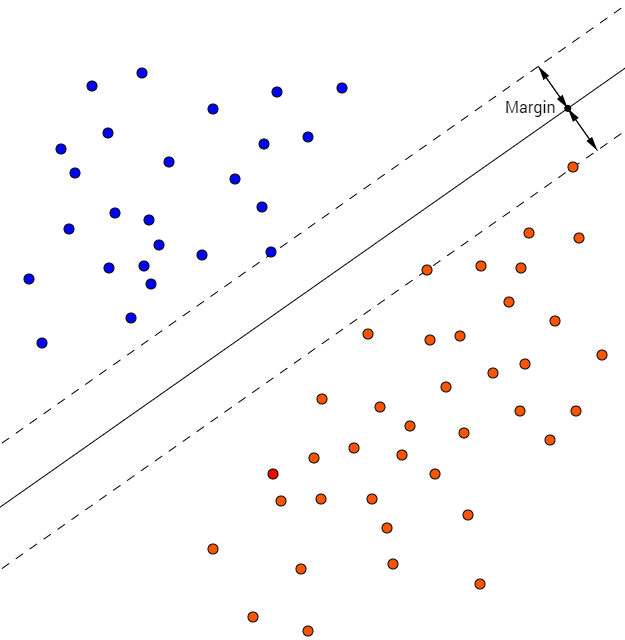
\includegraphics[width=\textwidth]{./figs/non_svm_classification_illustration}
        \caption{Non maximized margin separation}
        \label{fig:non_maximized_margin}
    \end{subfigure}
    \begin{subfigure}[b]{0.45\textwidth}
        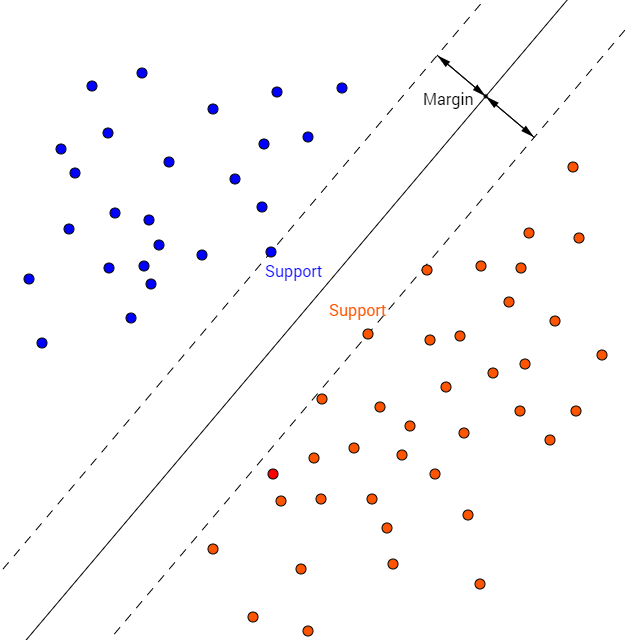
\includegraphics[width=\textwidth]{./figs/svm_classification_illustration}
        \caption{SVM maximized margin separation}
        \label{fig:svm_maximized_margin}
    \end{subfigure}
    \caption{Two possible results of linear binary classification}
    \label{fig:classification_comparison}
\end{figure}

Figure~\ref{fig:classification_comparison} illustrates two different ways of splitting the data into two classes. Figure~\ref{fig:non_maximized_margin} shows a non-maximized margin split, while Figure~\ref{fig:svm_maximized_margin} follows the \ac{svm} algorithm of finding the support vectors that result in the largest margin between the two segments. \\

The algorithm can also be used if linear separation of the training data is impossible. This could either be achieved by allowing misclassified points and introducing a slack variable, or by using the \textit{kernel trick}. In the first approach the misclassified points are assigned a penalty related to the distance away from the support vector of their class segment. The longer the distance, the higher the penalty. The penalty comes in the form of a positive slack variable, which governs the trade-off between misclassified points and the margin. \\

By using the \textit{kernel trick}, the data is mapped onto a higher dimensional space where it becomes linearly separable. This is done by applying a \textit{kernel function} to the data. The most popular kernel functions are the Radial Basis, the Polynomial and Sigmoidal kernels. The in-depth explanation of \ac{svm} by \cite{Fletcher09} states that finding the right kernel function is more of an art than an exact science. It often comes down to trial and error. \\

\begin{figure}[t]
    \centering
    \begin{subfigure}[b]{0.45\textwidth}
        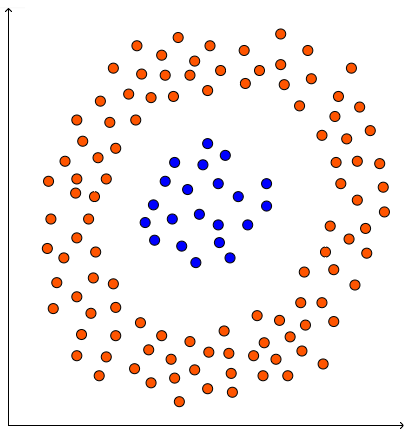
\includegraphics[width=\textwidth]{./figs/non_linearly_separable_classes}
        \caption{Before application of \textit{kernel trick}}
        \label{fig:non_linearly_separable_2d}
    \end{subfigure}
    \begin{subfigure}[b]{0.45\textwidth}
        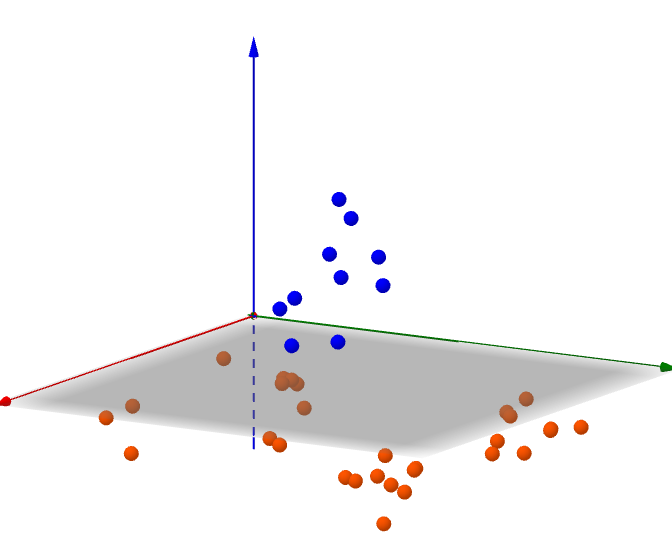
\includegraphics[width=\textwidth]{./figs/non_linearly_separable_classes_higher_dimension}
        \caption{After application of \textit{kernel trick}}
        \label{fig:non_linearly_separable_3d}
    \end{subfigure}
    \caption{\textit{Kernel trick} applied to a non-linearly separable dataset}
    \label{fig:non_linearly_separable_classes}
\end{figure}

Figure~\ref{fig:non_linearly_separable_2d} shows a dataset with a clear pattern which is not linearly separable. Figure~\ref{fig:non_linearly_separable_3d} shows the same dataset after being transformed by a kernel function to 3-dimensional space. The items occupy the same positions on the $xy$-plane, but are separable along the $z$-axis. \\

The \ac{svm} algorithm can also be applied to classification problems with more than two classes. To solve the multi-class classification problem, two methods, One-vs-All and One-vs-One, are commonly used. Both methods use a set of binary \ac{svm} classifiers and are thoroughly explained by \cite{HsuLin02}. Popular implementations of the \ac{svm} algorithm includes solving quadratic programming problems using a sequential minimal optimization algorithm invented by \cite{Platt98}.


\subsection*{Realization of the Classifier}
The classifier was realized using the Scikit-Learn framework which includes a series of \ac{svm} implementations. We chose the SVC variant, also known as C-Support \ac{svm} classifier, which is based around the idea of setting a constant $C$ that will be used to penalize incorrectly classified instances. High $C$ values will create a narrower margin, which will be able to classify more training elements correctly, but may also lead to overfitting. Therefore, it is desirable to perform some kind of parameter optimization to find the optimal $C$ value. For multi-class classification, Scikit-Learn uses the One-vs-One method, with a run time complexity quadratic to number of elements. However, this will not be a problem for the relatively small (under 10\thinspace000 elements) SemEval datasets. 


\section{Combining BaseClassifiers}
\subsection{Multi-Step Classifier}
\label{sec:multi_step_classifier}

\begin{figure}[t]
    \begin{center}
        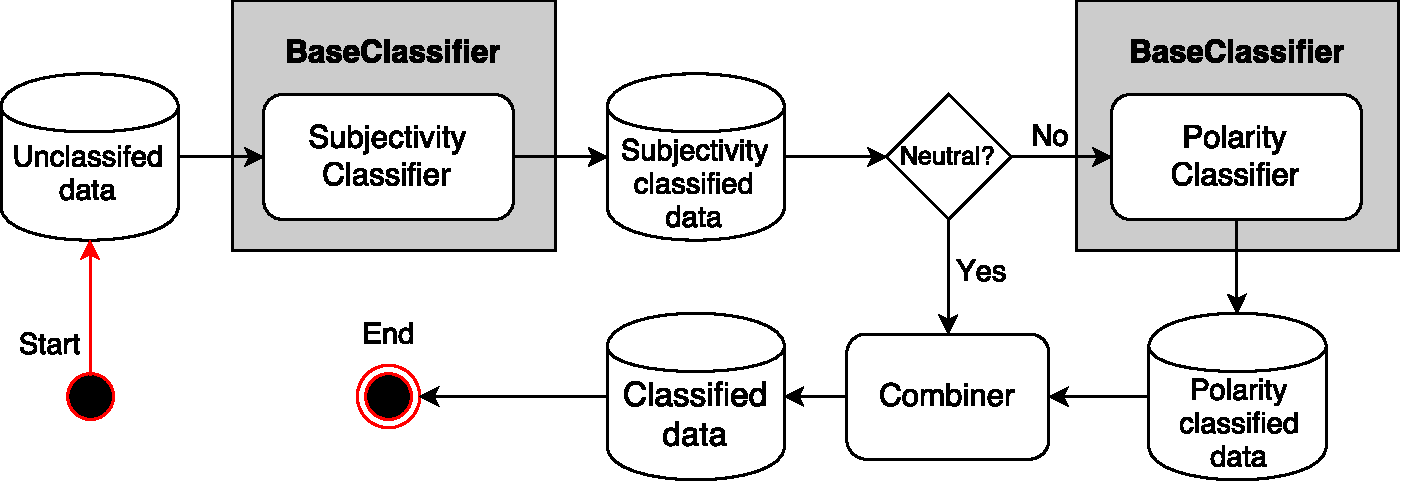
\includegraphics[width=\textwidth]{./figs/data_flow}
    \end{center}
    \caption{Data flow in the two-step classifier}
    \label{fig:data_flow}
\end{figure}

A single \textit{BaseClassifier} acts as a one-step classifier, but by chaining \textit{BaseClassifier}s sequentially, we can create a multi-step classifier. Each classifier can be trained independently on different data thereby learning a different classification function. Figure~\ref{fig:data_flow} illustrates how chaining of two \textit{BaseClassifier}s can create a two-step classifier. The first \textit{BaseClassifier} is trained only on data labeled as subjective or objective, while the second \textit{BaseClassifier} trains only on subjective data, labeled positive or negative. When classifying, if the first \textit{BaseClassifier} classifies an instance as subjective, the instance is forwarded to the second \textit{BaseClassifier} to determine if the instance is positive or negative. The results from both classifiers are then combined together and the final classifications are returned.

\subsection{Ensemble Classifier}
By combining the \textit{BaseClassifier}s in parallel, we can create an ensemble of classifiers. Each of the classifiers is independent of the others and all classify the same instances. At the end, the classifiers take a vote to decide on the final classification of the instance. Because the \textit{BaseClassifier}s are so general, it is possible to create \textit{BaseClassifier}s that extract different features, do different preprocessing and use different classification algorithms; we could combine them to create an ensemble system. 


\section{Results}
\label{sec:init_experiment_results}

\subsection{Test Results}
\label{sec:test_results}
In order to thoroughly test our system and its components, two main tests were conducted. A performance test of our final system with optimal parameters on all datasets, comparing the performance of our system against previous \ac{ntnu} developed \ac{tsa} systems, and an ablation study to identify the importance of the different features used in our system. 

\subsection*{Classifier Performance}
 Our \ac{tsa} system was trained on the \textit{\ac{semeval} 2013-train} training set, using the optimal parameters identified through a grid search, and tested on the \textit{\ac{semeval} 2013-test} and the \textit{\ac{semeval} 2014-test} test sets before being scored using the scoring metrics described in Section~\ref{sec:classification_scoring_metrics}. The results are shown in Table~\ref{tab:system_comparison} together with the results of the systems we aimed to improve. \\
 
 The performance of our system, compared to the previously \ac{ntnu} developed \ac{tsa} systems of \citep{FaretReitan, ReitanEtAl15} and \citep{SelmerBrevik, SelmerEtAl13} is very good. On the \textit{2013-test} set, we can see that our system performs better than \citeauthor{FaretReitan} and a lot better than \citeauthor{SelmerBrevik}. On the \textit{2014-test} set our system performs identical to \citeauthor{FaretReitan}, while still performing better than \citeauthor{SelmerBrevik}. However, an important aspect to notice is the execution time. Although we were not able to replicate the results of \citeauthor{FaretReitan} by running their system, we got a rough estimate of their execution time. On the \textit{2013-test} set their execution time was 180 seconds against our 74, and on the \textit{2014-test} set their time was 93 against our 41. Even though these execution time estimates are unofficial, they still indicate a reduction in execution time from their system to ours. Compared to the execution time of \cite{SelmerBrevik} our system is still quite slow, but the simplicity of their system also leads to a significantly lower performance.
 

\begin{table}[t]
    \centering
    \begin{tabular}{l|c|c|c|c|c|}
        \cline{2-6}
        & \textbf{System} & \textbf{Precision} & \textbf{Recall} & \textbf{F1-Score} & \textbf{Time} \\
        \cline{1-6}
        \multirow{3}{*}{\rot{2013}} & \citeauthor{SelmerBrevik} & 0.6787 & 0.6644 & 0.6482 & 0.36 \\
        \cline{2-6}
        & \citeauthor{FaretReitan} & 0.731 & 0.697 & 0.688 & \textasciitilde{}180 \\
        \cline{2-6}
        & \textbf{Initial Experiment} & 0.7209 & 0.7120 & 0.7073 & 74.01 \\
        \hhline{======|}
        
        \multirow{3}{*}{\rot{2014}} & \citeauthor{SelmerBrevik} & 0.7071 & 0.6667 & 0.6614 & 0.17 \\
        \cline{2-6}
        & \citeauthor{FaretReitan} & 0.738 & 0.684 & 0.684 & \textasciitilde{}93 \\
        \cline{2-6}
        & \textbf{Initial Experiment} & 0.7091 & 0.6832 & 0.6847 & 41.38 \\ \hline
    \end{tabular}
    \caption{Initial Experiment performance comparison}
    \label{tab:system_comparison}   
\end{table}

\subsection*{Ablation Study}
\label{sec:ablation_study}
In order to detect the overall importance or impact each feature has on our \ac{tsa} system, we conducted a simple ablation study. This was done by removing each feature in turn and checking how the performance of the system was affected. The results of the ablation study are shown in Table~\ref{tab:ablation_study}. \\

\begin{table}[t]
    \centering
    \begin{tabular}{|l|c|c|}
        \hline
        \textbf{Features} & \textbf{2013-test} & \textbf{2014-test} \\ \hline
        All                             & 0.7073 & 0.6847 \\ \hline
        All - Word $n$-grams            & 0.7050 & 0.6833 \\
        All - Character $n$-grams       & 0.6992 & 0.6812 \\
        All - Both $n$-grams            & 0.6948 & 0.6784 \\ \hline
        All - Automatic Lexica          & 0.7031 & 0.6888 \\
        All - Manual Lexica             & 0.7005 & 0.6905 \\
        All - All Sentiment Lexica      & 0.6862 & 0.6818 \\ \hline
        All - Word Clusters             & 0.7072 & 0.6825 \\ \hline
        All - Part-of-Speech tag counts & 0.7080 & 0.6879 \\
        All - Punctuation counts        & 0.7128 & 0.6946 \\
        All - Emoticons counts          & 0.7028 & 0.6826 \\ 
        All - All counts                & 0.7069 & 0.6787 \\ \hline
        All - VADER Sentiment           & 0.6960 & 0.6796 \\ \hline
    \end{tabular}
\caption[Ablation study results for the Initial Experiment]{Ablation study results. All - F means all features except for F. All values are $F_1$-scores.}
    \label{tab:ablation_study}   
\end{table}

As we can see, the single most important feature is the Sentiment Lexica. On the \textit{2013-test} set the accuracy of the system is reduced from 0.7073 to 0.6862 when the feature is removed. The effect of removing the Sentiment Lexica feature when tested on the \textit{2014-test} set is not as apparent. A possible cause of the difference in performance impact may be that most of the Sentiment Lexica used were created at the same time as the \textit{2013-test} set, and could possibly better reflect the language in that period of time. For the \textit{2014-test} it is less clear which feature is the best, collectively $n$-grams and all counts perform better, but VADER Sentiment is the single most important feature, reducing the accuracy from 0.6847 to 0.6796 when being removed. On the \textit{2013-test} set on the other hand, the VADER Sentiment feature does not have the same impact, but is still the second most important single feature. As VADER Sentiment was created in 2014, the cause of this difference may also be a change in how the language is used and that VADER Sentiment better reflects the language in 2014.  \\

The second most important features are the $n$-gram features. The removal of both character $n$-grams and word $n$-grams leads to a significant degradation in performance on both datasets. \\

Another interesting result is the impact of the features: Part-of-Speech counts and Punctuation counts. On both the \textit{2013-test} and the \textit{2014-test} sets, removal of those features causes slight improvement in performance, but when removed together with the Emoticon counts, the degradation in performance is larger than the performance degradation caused by only removing the Emoticon counts feature. A possible cause for this is that the classifier finds a pattern between all three of the counts that disappears when one of them is removed.


\subsection{SemEval 2016 Results}
We participated with the Initial Experiment system in \ac{semeval} 2016 subtask 4a: "Message Polarity Classification" under the team name \textit{NTNUSentEval} and ended up on the 11th place out of 34 competing systems, as shown in Table~\ref{tab:semeval_results}. \\

Our system was ranked as number 1 on the SMS dataset and as number 3 on the Live-Journal dataset. On the remaining datasets containing tweets, the system was ranked between 10th-13th place. The reason why our system performed so well on SMS and Live-Journal messages is unclear. A possible explanation may be that our system was only trained on the \textit{2013-train} dataset, while more than half the teams participating in SemEval 2016 also used large external tweet datasets, which could improve their performance on Twitter data, but also lead to worse performance on out-of-domain data. 

\glsresetall
%!TEX root = ../report.tex
\chapter{Architecture}
\label{cha:architecture}

To create a system for automatic creation of a sentiment lexicon, two different approaches have been developed based on the graph propagation approach and the \ac{pmi} approach, outlined in Section~\ref{sec:automatic_generation_of_sentiment_lexica}. In addition, a lexicon based classifier has been developed, utilizing the features of the lexicon created. In this chapter the three systems are described individually in addition to two core system components: tweet preprocessor and vocabulary tokenization, used in all three systems. After initial tests of the two lexicon creation approaches, the \ac{pmi} approach outperformed the graph propagation approach and became our main focus of the two. This is specifically reflected in a more sophisticated $n$-gram creation process. 


\section{Tweet Preprocessor} 
\label{sec:tweet_preprocessor}
Our system implements preprocessing as a set of simple functions, each taking in a string, performing a simple operation, and returning the resulting string. This simple design allows chaining several preprocessors one after another achieving complex results, while remaining easily reusable because of the simplicity of each single preprocessor. Additionally, we implement two ways of chaining the preprocessors: by text or by word. A set of preprocessors chained together by text will perform the filter operation on the entire text, while preprocessors chained together by word will perform the operation at word level and will ignore words marked as "protected".\footnote{In our implementation a word is marked as protected if it begins and ends with "||".} This is particularly important with emoticons, as we often want to remove non-alphanumeric signs from the text, and most emoticons contain non-alphanumerical signs. With this approach we can first identify all the emoticons, mark them as "protected", and then apply the remove non-alphanumerical signs preprocessor at word level. This will remove all non-alphanumerical signs except the ones that are part of an emoticon. \\

\begin{figure}[t]
    \centering
    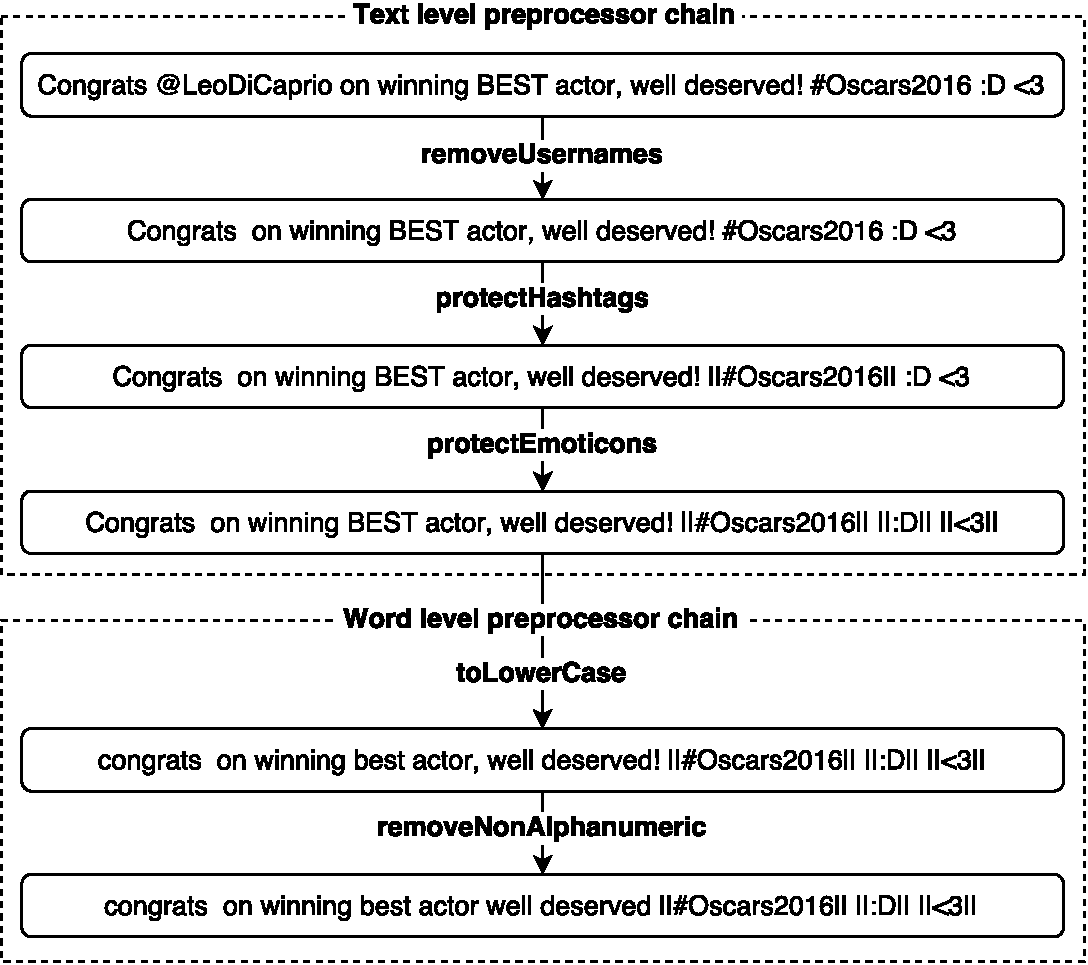
\includegraphics[width=\textwidth]{./figs/chain_preprocessor}
    \caption{Effect of different preprocessors on a tweet}
    \label{fig:chain_preprocessor}
\end{figure}

Figure~\ref{fig:chain_preprocessor} illustrates a series of text-level and word-level preprocessors chained one after another. Notice how hashtags are still intact and upper-cased after the $removeNonAlphaNumeric$ and $toLowerCase$ preprocessors because they were marked as "protected" and therefore ignored. \\

\begin{table}[t]
    \setlength\tabcolsep{2pt}
    \begin{tabular}{| l | p{8.3cm} |}
        \hline
        \textbf{Filter} & \textbf{Description} \\ \hline
        %HTMLUnencode
        normalizeForm & Normalizes letters to Latin alphabet if possible, for example "Déjà vu" becomes "Deja vu" \\ \hline
        unicodeEmojisToAlias & Translates Unicode emoji characters to their alias as given by emoji-java library \\ \hline
        removeUnicodeEmojis & Removes all Unicode emoji characters \\ \hline
        protectEmoticons & Marks all ASCII emoticons as "protected" \\ \hline
        removeEmoticons & Removes all ASCII emoticons \\ \hline
        removeUsername & Removes all username mentions \\ \hline
        removeEMail & Removes all e-mail addresses \\ \hline
        removeHashtag & Removes all hashtags \\ \hline
        protectHashtag & Marks hashtags as "protected" \\ \hline
        removeRTTag & Removes RT tags \\ \hline
        removeURL & Removes URLs \\ \hline
        %removeApostrophes & Removes characters often found mid word, such as '
        removeNonSyntact & Removes all non alphabetic or punctuation characters \\ \hline
        removeNonAlphanum & Removes all non alphanumerical characters \\ \hline
        %removeFreeDigits & Removes 
        toLowerCase & Transforms all letters to lower case \\ \hline
    \end{tabular}
    \caption{List of preprocessors used in our system}
    \label{tab:master_filters}
\end{table}

\subsection*{Elongation Correction}
\begin{figure}[t]
    \fbox{\parbox{\textwidth}{
    \begin{enumerate}
        \item For every word in the vocabulary, extract the condensed form, where sequences of a repeated letter are replaced with a single instance of that letter.\\
        E.g., \textit{niiiice → nice, realllly → realy, ...}
        \item Create sets of words sharing the same condensed form.\\
        E.g., \{\textit{nice, niiice, niccccceee, ...}\}, \{\textit{realy, really, realllly, ...}\}
        \item Remove sets which contain 5 or less unique variations.\\
        E.g., \{\textit{committee, committe, commitee}\}
        \item From each set, remove words with distribution less than 5\% among the words that are condensed to the same form.\\
        E.g., \{\textit{god: 15\%, good: 80\%, goood: 2\%, godd: 1\%, goood: 1\%, gooood: 1\%, ...}\} → \{\textit{god: 15\%, good: 80\%}\}
    \end{enumerate}}}
    \caption{Steps in the creation of a condensed form dictionary}
    \label{fig:canonical_dict}
\end{figure}

To handle elongation, described in Section~\ref{sec:text_filtering}, a correction process utilizing the Levenshtein distance algorithm (Section~\ref{sec:levenshtein}) and the condensed form of words, is applied to all words. The process consists of two parts: a four step dictionary creation part inspired by \cite{brody11}, shown in Figure~\ref{fig:canonical_dict}, and a word correction part using the created dictionary. In order to correct a word, the word is first reduced to its condensed form, before being looked up in the dictionary. If found, the dictionary returns the most likely spellings of the initial word. Then the Levenshtein distance is calculated between the initial word and each of the returned words, before correcting the initial word to the closest match. This way, with a dictionary containing both "good" and "god", the word "goddd" is 2 removals away from "god" or 2 removals and 1 addition from "good", and will therefore be reduced to "god".

\section{Vocabulary Tokenization}
\label{sec:tokenization}
In both our lexicon based classifier and our \ac{pmi} lexicon approach the process of tokenization is used. The process consists of splitting sentences into what we call "optimal" tokens, which are the longest non-overlapping $n$-grams also found in a given vocabulary. The $n$-grams that were not found in the provided vocabulary are tokenized as unigrams. The vocabularies used should contain the most relevant $n$-grams within the given context. The longest $n$-grams are preferred based on the assumption that the longer $n$-grams provide more precise information than the shorter $n$-grams. \cite{Goodman01abit} argues that there is little to gain with $n$-grams longer than $n=5$, stating that the performance, in terms of perplexity and entropy of the language model, plateaus between $n$-grams of length 5-7. \citeauthor{Goodman01abit} further states that building a model based on $n$-grams of lengths up to $n=5$ appears to give a good tradeoff between computational resources, in terms of runtime and memory usage, and performance.  \\

\begin{figure}[t]
    \centering
    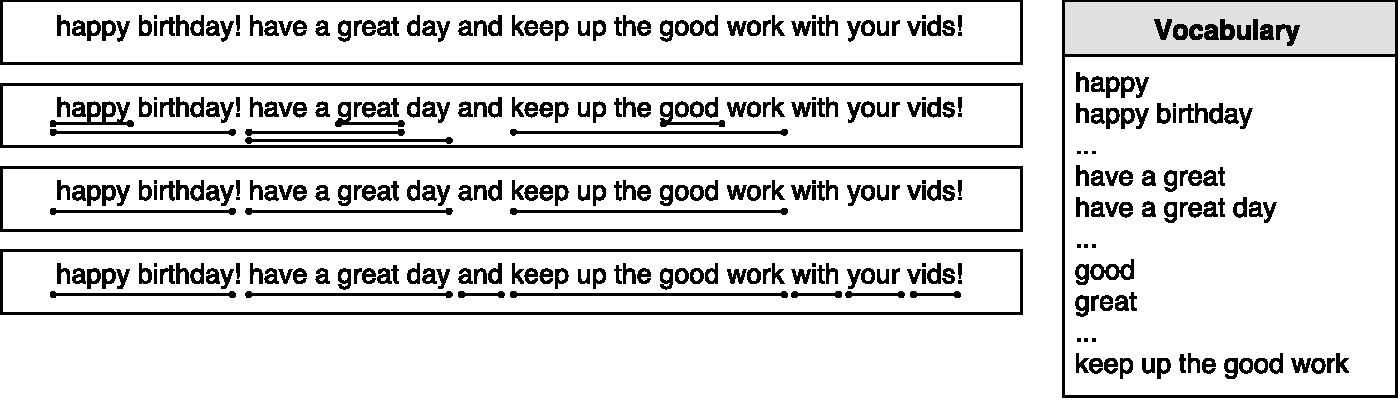
\includegraphics[width=\textwidth]{./figs/tweet_tokenization}
    \caption{The tokenization process shown step by step}
    \label{fig:tweet_tokenization}
\end{figure}

Figure~\ref{fig:tweet_tokenization} illustrates the process of vocabulary tokenization of a tweet. The different stages of tokenization of a tweet are shown on the left, while the relevant phrases in the vocabulary are shown on the right. The first stage of vocabulary tokenization is to find all $n$-grams in the tweet that are also present in the vocabulary. Then, we select the longest $n$-gram found and remove all the $n$-grams that overlap with it. The final stage is to tokenize the remaining words in the tweet as unigrams. The reason for keeping the words not present in the vocabulary is that these words may be intensifiers or negators, which are excluded from our lexicon. Additionally, keeping these words is important for negation, since it affects the $x$ next words.

\section{Tweet Streaming API Dataset}
\label{sec:twitter_streaming_dataset}
\subsection*{Raw Tweets}

\begin{figure}[t]
    \centering
    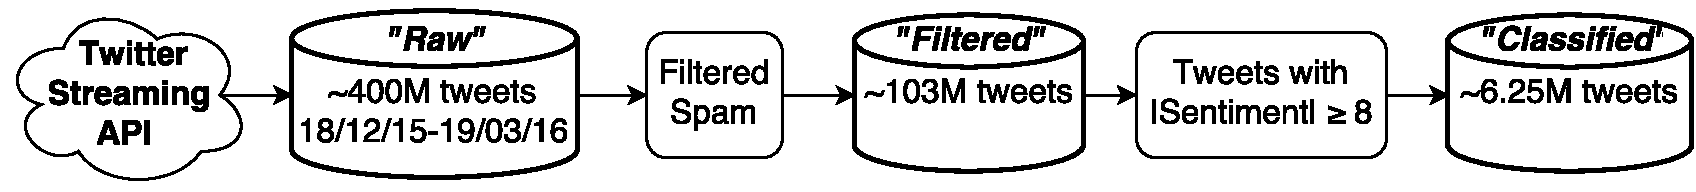
\includegraphics[width=\textwidth]{./figs/twitter_datasets}
    \caption{Datasets created using Twitter Streaming API}
    \label{fig:twitter_steaming_api_datasets}
\end{figure}


To be able to create a sentiment lexicon based on raw tweets, a large corpus of tweets was needed. We downloaded about 400 million tweets using the Twitter Streaming API.\footnote{\url{https://dev.twitter.com/streaming/reference/post/statuses/filter}} The tweets were gathered in the period 18/12/2015-19/03/2016 (92 days), with about 4 million tweets downloaded each day.

\subsection*{Filtered Dataset}
\label{sec:filtered}
After that, we filtered the entire raw tweets dataset, removing all tweets considered to be noise. A tweet was considered to be noise if:

\begin{itemize}
    \item Contained "RT @"
    \begin{itemize}
        \item Nearly half of all downloaded tweets were retweets, most of the retweets are of few original tweets, failing to remove these would make some phrases over-represented.
    \end{itemize}
    \item Contained a URL
    \begin{itemize}
        \item Tweets containing a URL were usually response to, opinion of or simply the first ~100 characters of a news story. These tweets are generally unhelpful to analyze without also analyzing the contents of page linked to itself. 
    \end{itemize}
    \item Contained $^{\circ}$ symbol
    \begin{itemize}
        \item There is a surprising amount of automated weather and GPS services connected to Twitter that regularly tweet current weather or location, this simple rule excludes most of them.
    \end{itemize}
    \item Ended with a number
    \begin{itemize}
        \item Spammers often tweet the same message over and over with an incrementing number attached to the end of the tweet, this is probably to combat Twitter's own automatic spam detection.
    \end{itemize}
\end{itemize}

The resulting dataset contained about 103 million tweets and is used to generate the $n$-grams.\\

\subsection*{Labeled Dataset}
\label{sec:labeled}
To be able to use the \ac{pmi} approach when creating a sentiment lexicon, a large dataset of labeled documents --- or in our case labeled tweets --- was needed. For the approach to produce good and reliable results, the amount of labeled tweets we needed was much higher than the manually annotated tweets made available through \ac{semeval}, which in turn meant that we needed a method for labeling tweets ourselves. \\

The approach we came up with was to label tweets using our lexicon based sentiment analysis system, described in Section~\ref{sec:lexicon_based_sentiment_analysis_system} with the manually annotated sentiment lexicon \textit{AFINN} by \cite{AFINN}. For the labeling to be as accurate as possible, only tweets with absolute sentiment score above a certain value were labeled and extracted. The value chosen was found using grid search and is a trade-off between precision and recall. Low values will give higher recall as we will be able to classify more tweets, but it will also lower precision. \\

Based on the \textit{Filtered} dataset, with 103 million unlabeled tweets, the labeling process yielded a labeled dataset containing 6.25 million tweets, of which 58.7\% were labeled as positive and the remainder as negative.


\section{Automatic Lexicon Creation}
In order to achieve the goal of automatic creation of a sentiment lexicon, two different approaches, both identified during our literature review presented in Section~\ref{sec:automatic_generation_of_sentiment_lexica}, have been developed. The developed approaches are based on the graph propagation lexicon described in Section~\ref{sec:graph_propagation_algorithm} and the \ac{pmi} lexicon described in Section~\ref{sec:pointwise_mutual_information}. 


\subsection{Graph Propagation Lexicon}
\label{sec:graph_propagation_lexicon}
Our implementation of the graph propagation approach consists of four steps. A vocabulary identification step, a context-vector creation step, a graph creation step and finally a sentiment propagation step.   


\subsection*{Vocabulary Identification}
During the vocabulary identification step a set of candidate $n$-grams are identified and selected, forming a context vocabulary. Each tweet is processed into all possible $n$-grams with length up to $n=5$, where candidate $n$-grams are selected based on their occurrence frequency in the large unlabeled \textit{Filtered} dataset. All $n$-grams below a frequency threshold, in addition to all $n$-grams ending on one of the stopwords in Table~\ref{tab:master_stopwords} or containing one of the intensifiers in Table~\ref{tab:intensifiers} are filtered out. Infrequent $n$-grams are filtered out, because the context vector to be created in the subsequent step is too unreliable on infrequent $n$-grams. In contrast to \cite{MohammadKZ2013}, where all $n$-grams containing stopwords are removed, we only remove $n$-grams ending on a stopword. This is because we believe that the ending stopword does not provide the $n$-gram with any additional information, but $n$-grams starting with or containing a stopword may change the $n$-grams sentiment or reverse it completely. For example, \textit{"the best"} is more positive than just \textit{"best"}, and the phrase \textit{"the shit"}, which is a positive phrase, is captured in addition to the word \textit{"shit"}, which on its own is negative. $N$-grams containing intensifiers were removed due to the fact that the automatic lexicon creator was developed in parallel to our lexicon based classifier. The classifier namely detects and uses intensifiers in the classification process as described in detail in Section~\ref{sec:lexicon_based_sentiment_analysis_system}. The resulting context vocabulary forms a collection of all candidate entries for the sentiment lexicon to be created in the following steps.  


\subsection*{Context Vector Creation}
\label{sec:context_vector}
To be able to compare the candidate $n$-grams against each other, a context vector is created for all of them. This is achieved by following the COALS method presented by \cite{Rohde06animproved}. The context vector of an $n$-gram is created by summing up the word frequencies of the $x$ number of words occurring to the left and $x$ number of words to the right of the $n$-gram over all mentions of the $n$-gram in the dataset. For the context vectors, representing the context of the $n$-gram, to be as accurate as possible, the context vector word frequencies are weighted according to the distance away from the $n$-gram. This is done using a ramped window of size 6. A word appearing right next to the $n$-gram on either side will increase the frequency of that word in the context vector by 6 for that side, while a word appearing six words away will increase the frequency by 1 for that side, as shown in Figure~\ref{fig:ramped_window}. 

After all initial context vectors have been created, a matrix containing all $n$-grams is created. In the matrix each row contains the context vectors of all selected $n$-grams and each column contains the occurrence frequency of a single word occurring in the different vectors. When the matrix has been initialized, the values are normalized using Pearson Correlation as described in Section~\ref{sec:pearson_correlation}. Finally, all negative values are set to 0, while all positive values are squared, resulting in our final context vectors. \\

\begin{figure}[t]
    \centering
    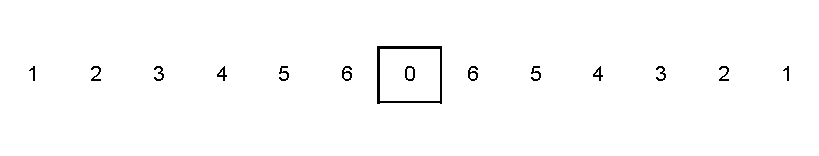
\includegraphics[width=\textwidth]{./figs/ramped_window}
    \caption[Ramped window of size 6]{Ramped window of size 6. The square represents an occurrence of an $n$-gram in a sentence. The numbers on either side represents the weights of the surrounding words.}
    \label{fig:ramped_window}
\end{figure}


\subsection*{Graph Creation}
When all candidate entries have been selected and their respective context vectors have been calculated, the graph is created. The graph consists of nodes, representing the candidate entries, and edges with weights, representing the similarity between the nodes. In order to create the edges, the similarity between all pairs of $n$-grams, represented by their context vectors, is calculated using the cosine similarity measure as described in Section~\ref{sec:cosine_similarity}. Following the approach suggested by \cite{Velikovich2010}, an edge is created between two nodes if their cosine similarity is greater then a predefined threshold. The edge weights of the created edges are set to the calculated cosine similarity. 

\subsection*{Sentiment Propagation}
Using the Graph Propagation algorithm outlined in Section~\ref{sec:graph_propagation_algorithm}, the seed nodes propagate their sentiment values through the finished graph. In our implementation, each seed node can affect nodes that are connected to it via two or less other nodes. When all seed nodes have propagated their sentiment value, the final sentiment value of each node is calculated by subtracting the sum of all negative max paths from the sum of all positive max paths. The negative and positive max paths to a node, are the maximum sentiment values each connected seed node affects the node with. A node with more paths to positive than negative seed nodes, will most likely get a positive sentiment value. Nodes with few paths to seed nodes, or an approximately equal number of paths to both positive and negative seed nodes are likely to get a sentiment value close to zero. Finally, the lexicon is created by extracting all the $n$-grams and their sentiment values. 

\subsection{PMI Lexicon}
\label{sec:pmi_lexicon_creation}
Similarly to our implementation of the Graph Propagation approach, our \ac{pmi} lexicon approach is divided into a series of steps consisting of vocabulary identification, counting vocabulary occurrences in a polarized dataset and sentiment calculation, as illustrated in Figure~\ref{fig:creator_overview}.
\begin{figure}[t]
    \centering
    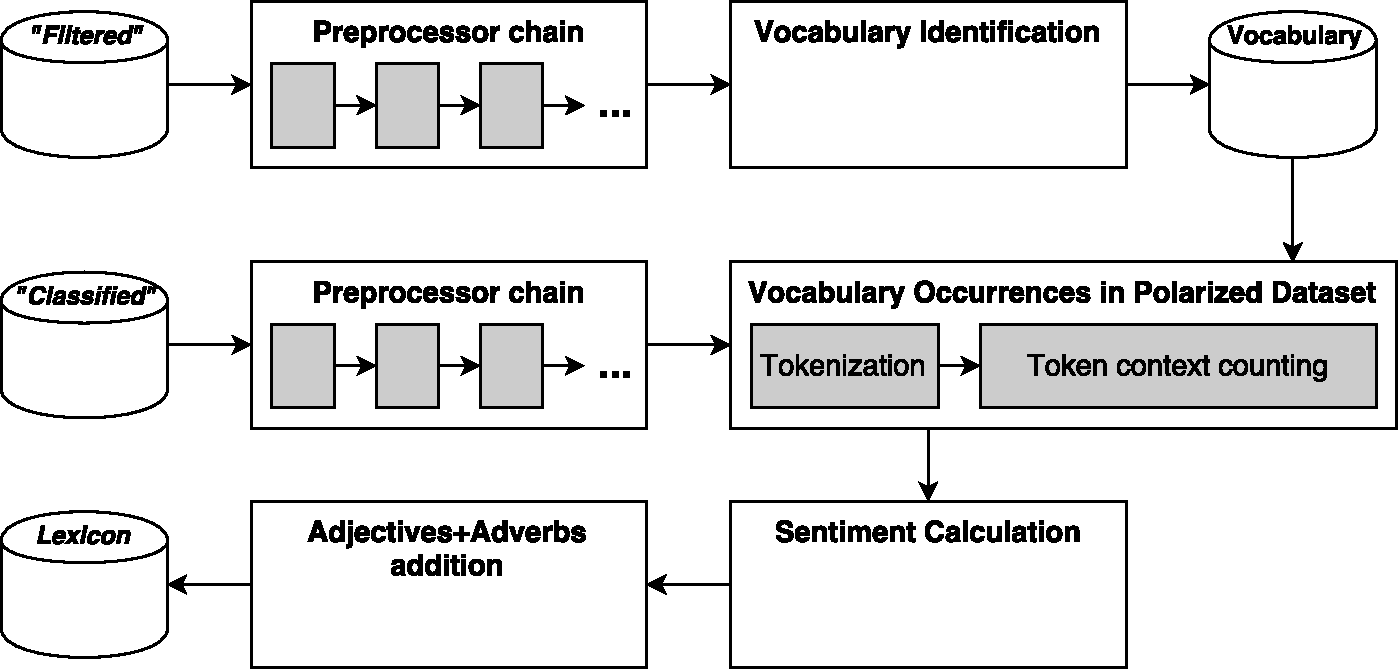
\includegraphics[width=\textwidth]{./figs/creator_overview}
    \caption{Architecture of the PMI lexicon creation system}
    \label{fig:creator_overview}
\end{figure}

\subsection*{Vocabulary Identification}
Similarly to the vocabulary identification step in Section~\ref{sec:graph_propagation_lexicon}, the \ac{pmi} lexicon vocabulary identification step also extracts and selects candidate $n$-grams for a context vocabulary based on the large unlabeled \textit{Filtered} dataset. However, the process of selection is quite different. Whereas the selection process in our graph propagation approach is strictly based on $n$-gram frequency, the selection process in our \ac{pmi} lexicon implementation uses the \ac{pmi} $n$-grams, method described in Section~\ref{sec:pointwise_mutual_information}. For an $n$-gram with $n>1$ to be selected, the \ac{pmi} of the included words needs to be higher than a predefined threshold. This way only $n$-grams containing words that together mean something or form a common phrase are selected. In addition, $n$-grams ending on a stopword or containing intensifiers are filtered out the same way as described in Section~\ref{sec:graph_propagation_lexicon}. Unigrams are not selected as candidate entries for the context vocabulary in this process, but are introduced to the system in the following two steps. \\

\begin{figure}[t]
    \centering
    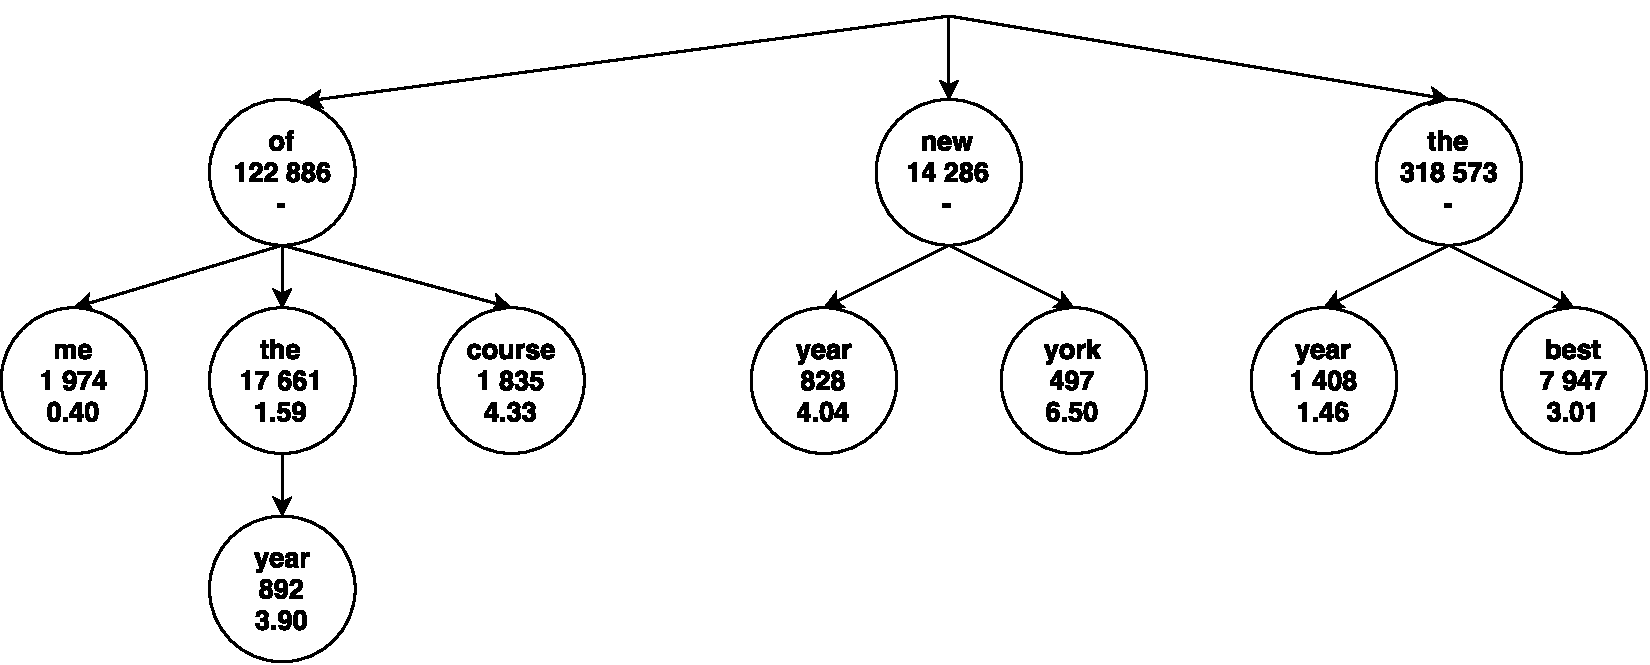
\includegraphics[width=\textwidth]{./figs/token_trie}
    \caption{Segment of a $n$-gram trie}
    \label{fig:trie}
\end{figure}

Figure~\ref{fig:trie} illustrates the process of identifying the vocabulary. Our implementation uses the trie data structure to count the number of occurrences of $n$-grams. The second line in each node is the number of times the $n$-gram has occurred in the dataset, while the third line is the $n$-gram's \ac{pmi} value. The $n$-gram "of me" is more frequent than "of course", but "of course" has much higher \ac{pmi} value. By setting two thresholds, one for frequency and one for \ac{pmi}, we can extract only the meaningful $n$-grams.

\subsection*{Vocabulary Occurrences in Polarized Dataset}
In order to calculate sentiment values of $n$-grams in our context vocabulary, the \textit{Labeled} dataset is used. For each entry in the dataset the tokenization process, described in Section~\ref{sec:tokenization}, is applied, splitting the entries into "optimal" tokens. The "optimal" tokens are the longest possible non-overlapping $n$-grams found in the context vocabulary created in the previous step. Each individual token holds counters for occurrences in positive and negative contexts. The positive context counter for a token is incremented by 1 for each time the token appears in an entry labeled as positive and the same applies for the negative context counter for tokens appearing in negative entries. The counting process utilizes the same trie data structure used when identifying the vocabulary in the previous step.


\subsection*{Sentiment Calculation}
For each $n$-gram in the context vocabulary, a sentiment value is calculated. This is achieved by using the number of times each $n$-gram occurs in positive tweets and in negative tweets found in the previous step and apply Equation~\ref{eq:sentiment_score_final} as described in Section~\ref{sec:pointwise_mutual_information}. $N$-grams occurring more frequently in negative tweets than in positive will get a negative score, while $n$-grams occurring more frequently in positive tweets will get a positive score. $N$-grams occurring just as frequent in positive tweets as in negative tweets will get a score close to zero. Finally, the lexicon is created by adding all $n$-grams with absolute sentiment value above a defined sentiment value threshold and an occurrence frequency in the \textit{Labeled} dataset above a set frequency.

\subsection*{Adjective and Adverb Addition}
With the created lexicon from the previous step, all unigrams are run through an adjective and adverb addition algorithm, adding all missing adjective and adverb forms of the unigram to increase the coverage of the lexicon. The missing adverbs and adjective forms are derived based on a set of rules\footnote{Forming Comparative and Superlative Adjectives:\\ \url{http://www.eflnet.com/tutorials/adjcompsup.php} \\and Forming Adverbs from Adjectives:\\ \url{http://www.edufind.com/english-grammar/forming-adverbs-adjectives/}} and are added to the lexicon only if they were previously encountered in the above tokenization process. The newly added adverbs and adjectives are assigned the same sentiment value as their related $n$-gram, based on the assumption that most adverbs and adjective forms of an adjective convey approximately the same sentiment. The resulting lexicon forms the final \ac{pmi} lexicon.

\section{Lexicon Based Sentiment Analysis system}
\label{sec:lexicon_based_sentiment_analysis_system}
The lexicon based Sentiment Analysis system accepts single tweets or a set of tweets and outputs a predicted classification per tweet. The predicted classification is determined by running each tweet through three main stages: preprocessing, analysis and classification, as shown in Figure~\ref{fig:classifier_overview}.

\begin{figure}[t]
    \centering
    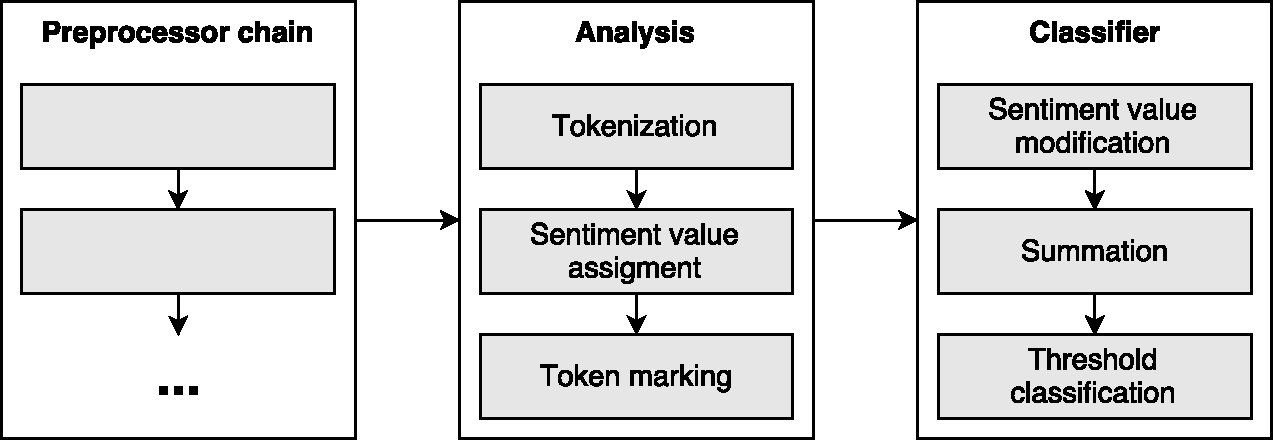
\includegraphics[width=\textwidth]{./figs/classifier_overview}
    \caption{Architecture of the lexicon classifier system}
    \label{fig:classifier_overview}
\end{figure}

\subsection*{Analysis}
After a tweet has been preprocessed, as described in Section~\ref{sec:tweet_preprocessor}, the resulting preprocessed tweet is analysed. The analysis consists of detecting negation cues, intensifier words as well as the use of punctuation marks such as: "!" and "?", and assigning sentiment values. This is done by first applying the tokenization process (Section~\ref{sec:tokenization}), splitting the preprocessed tweet into optimal tokens using the provided sentiment lexicon as vocabulary. Then the optimal tokens are looked up in the provided sentiment lexicon and assigned the lexicon value given its existence. Tokens are then marked, that is, each token is checked against a list of negation cues and intensifier words. If a token matches one of the negation ques, the following $x$ tokens are marked as negated. If a token matches an intensifier word, the next token is marked as intensified. Finally, a sentence ending in "!" or "?" will mark all the tokens in the sentence as intensified.


\subsection*{Classification}
Based on the information retrieved in the analysis step, the tweet is classified. The tokens are traversed and a classification value is calculated as a sum of the sentiment values of the individual tokens. The individual token's sentiment value depends on three variables: lexicon sentiment value of the token, whether or not the token was marked as in a negated context, and whether or not the token was marked as being intensified. If a token does not exist in the lexicon, its sentiment value is zero. The sentiment value of each token found in the lexicon is calculated as follows:

\begin{equation}
    Token Sentiment Value(token) = (L \cdot I) - N
    \label{eq:token_sentiment}
\end{equation}
where $L$ is the lexicon value of the token, $I$ is the intensification value of the token and $N$ is the negation value. When a token is not intensified $I=1$. When a token is not negated $N=0$. \\

The value of $I$ for a token is dependent on what intensifier word or punctuation mark it is affected by. Some intensifier words such as \textit{"kind of"} or \textit{"hardly"} will work as a dampeners with $I$-values between 0 and 1. Words like \textit{"incredibly"} or \textit{"extremely"} will on the other hand work as boosters with $I$-values above 1. A token can be intensified by both an intensifier and a punctuation mark. In such case, $I$ is the product of the intensification constant of the intensifier and the intensification constant of the punctuation mark. The $I$-values of "!" and "?" and the $N$ value along with their influence ranges are determined through the grid search. \\

The final sentiment score of a tweet is then calculated based on the sentiment values of the tokens:

\begin{equation}
    Tweet Sentiment Value = \sum\limits_{i=1}^{n} Token Sentiment Value(n)
\end{equation}

Finally, a tweet is classified as either positive, negative or neutral by comparing the $TweetSentimentValue$ against two thresholds, if the value is lower than $LowerNeutralThreshold$, the tweet is classified as negative, if the value is higher than $HigherNeutralThreshold$, the tweet is classified as positive, otherwise the tweet is classified as neutral. The thresholds are also determined through the grid search.

\glsresetall


%!TEX root = ../report.tex
\chapter{Experiments}
\label{cha:experiments}
In order to thoroughly test our lexicon based classifier and our PMI lexicon, a series of experiments were conducted. Both to determine how well our classifier, utilizing the PMI lexicon, fared against other more complex classifiers, and to check the effect of using our classifier as a feature in a machine learning classifier. We also experimented with lexica of different sizes, and compared our system to the competing systems of SemEval 2016. Finally, we performed an ablation study to determine the most important features of both our lexicon creation process and our classification process.

\section{Transition from Graph to PMI}
\label{sec:transition_graph_pmi}
Through the initial phases of this thesis work, the graph propagation approach was our main and only lexicon creation approach. However, we encountered several problems with the graph approach: 
\begin{itemize}
    \item \textbf{Creating the seed set:} Since the value of all words in the lexicon are decided by their similarity to the words in the seed set, it is crucial to get the seed set right. A small seed often produced smaller lexica with weaker sentiment values since fewer words were propagating the values, while a large seed set often had problems with setting good starting sentiment values. For example, \textit{"good"}, \textit{"great"}, and \textit{"outstanding"} are all positive words, but their sentimental strength is different.
    \item \textbf{Creating the context vector:} The similarity between $n$-grams is calculated as similarity between their context vectors, described in Section~\ref{sec:context_vector}. While this approach may work for unigrams, the relationship between mutli-grams and their neighboring words is less clear.
    \item \textbf{Computational complexity of similarity measure:} Our implementation relied on calculating the cosine similarity for each word with every other word. This means that the overall computational complexity was exponential. In practice, we could not create any lexica with more than 8\thinspace000 elements.
    \item \textbf{Context similarity vs. Sentiment similarity:} Finally, context similarity is not always correlated with sentiment similarity. For example, the word \textit{"good"} and the word \textit{"bad"} are often used in similar contexts, \textit{"the weather is good/bad"}, \textit{"I'm good/bad at reading"}. 
\end{itemize}

After approximately two months of development without satisfactory results, we decided to try out the PMI approach identified through our research. After only a couple of days of development, the PMI approach outperformed our graph propagation approach, as shown in Table~\ref{tab:graph_vs_pmi}, which in turn led us to changing our main lexicon creation approach over to the PMI approach. Throughout the remainder of this chapter, only the lexica created through our PMI approach are tested in addition to the lexicon based classifier.

\begin{table}[t]
    \centering
    \begin{tabular}{|l|c|c|c|c|}
        \hline
        \textbf{System} & \textbf{2013} & \textbf{2014} & \textbf{2015} & \textbf{2016} \\ \hline
        Graph approach  & 0.4942 & 0.4844 & 0.4571 & 0.4744 \\ \hline
        PMI approach    & 0.6130 & 0.6170 & 0.5711 & 0.5685 \\ \hline
    \end{tabular}
    \caption[Early results of graph approach vs. PMI approach]{Early test results of graph approach vs. PMI approach tested on the 2013-2016 SemEval datasets.}
    \label{tab:graph_vs_pmi}   
\end{table}

\section{Grid Search}
\label{sec:grid_search}
For our system to perform as well as possible, we needed to find the optimal parameters. That included finding the optimal parameters for both our lexicon creator and our classifier, listed in Table~\ref{tab:lexicon_creator_parameters} and Table~\ref{tab:lexicon_classifier_parameters}. Because optimal classifier parameters depend on the particular lexicon being used, which again depends on the lexicon creator parameters, we needed to create our own grid search method for our thesis system. The method we ended up with was not a complete grid search where all combinations of parameter values are explored, but instead a simpler, iterative parameter search. The search consisted of a series of iterative steps, where we in each step tested all predefined values of a single parameter, while keeping all the other variables constant, in search of the value that provided the best result. When we were not able to improve the result by changing any of the parameter values, the search was done. Because we were not testing all possible combinations of values, the parameters found may be a local maximum, but the trade-off was necessary since testing each combination took 3 minutes on average.

\begin{table}[t]
    \setlength\tabcolsep{2pt}
    \begin{tabular}{| l | p{9cm} |}
        \hline
        \textbf{Parameter} & \textbf{Description} \\ \hline
        maxNGramLength & Longest $n$-gram to include in vocabulary \\ \hline
        minNGramFreq & Minimum $n$-gram occurrence frequency to include in vocabulary \\ \hline
        minNGramPMI & Minimum $n$-gram PMI value to include in vocabulary \\ \hline
        minOccurrence & Minimum $n$-gram occurrence in polarized dataset to include in lexicon \\ \hline
        minSentiment & Minimum $n$-gram absolute sentiment value to include in lexicon \\ \hline
    \end{tabular}
    \caption{List of lexicon creator parameters}
    \label{tab:lexicon_creator_parameters}
\end{table}

\begin{table}[t]
    \setlength\tabcolsep{2pt}
    \begin{tabular}{| l | p{9cm} |}
        \hline
        \textbf{Parameter} & \textbf{Description} \\ \hline
        negationValue & The negation constant $N$ in Equation~\ref{eq:token_sentiment} \\ \hline
        exclamationIntensifier & Intensification constant for tokens inside sentence ending with an exclamation mark \\ \hline
        questionIntensifier & Intensification constant for tokens inside sentence ending with a question mark \\ \hline
        negationLength & Number of tokens after a negation cue that are considered negated \\ \hline
        classThreshLower & Threshold between the \textit{negative} and the \textit{neutral} sentiment classification \\ \hline
        classThreshHigher & Threshold between the \textit{neutral} and the \textit{positive} sentiment classification \\ \hline
    \end{tabular}
    \caption{List of lexicon classifier parameters}
    \label{tab:lexicon_classifier_parameters}
\end{table}

\section{Quality of SemEval Datasets}
\label{sec:criticism_semeval}
Through system tests performed during development, the SemEval 2016 results and the final system tests described in the following section, our scepticism towards the overall quality of the SemEval datasets of 2015 and 2016 in particular, was sparked. As discovered in the following section as well as through the SemEval 2016 results, the performance of all the classifiers drops drastically from the tests on the 2013 dataset to the 2016 dataset. This in turn led us to perform a few experiments on the datasets to see if we could back up our suspicions of a lower quality of the 2015 and 2016 SemEval datasets. We started our experiments by finding the number of duplicate tweets in the four datasets. For the datasets with duplicate tweets we checked whether or not the duplicate tweets were given the same classification label and counted the number of duplicates with different labels. \\

\begin{table}[t]
    \centering
    \begin{tabular}{|l|c|c|}
        \hline
        \textbf{Dataset} & \textbf{Duplicates} & \textbf{Different Classification}\\ \hline
        2013-test & 1.62 & 0.32 \\ \hline
        2014-test & 0.00 & 0.00 \\ \hline
        2015-test & 6.94 & 2.09 \\ \hline
        2016-test & 3.88 & 1.36 \\ \hline
    \end{tabular}
    \caption[SemEval dataset experiments]{SemEval dataset experiments, all values are per thousand tweets}
    \label{tab:dataset_experiments}   
\end{table}

As we can see from Table~\ref{tab:dataset_experiments} there are only 1.62 duplicated tweets per thousand tweets in the 2013 dataset and none in the 2014 dataset. In addition only 0.32 tweets per thousand found in the 2013 dataset had different classification label. For the two other datasets on other hand, we found significantly more duplicates that were classified differently. However, the amount of duplicated tweets with different classification is in comparison to the dataset size relatively small, and will on its own not impact the results noticeably. More importantly the numbers point to a possible preference difference among the used annotators, when it comes to what they assume is a polarized tweet (positive or negative) and what is a neutral tweet. The method of collecting and annotating tweets, described by \cite{SemEval:2016:task4}, has stayed the same since 2013, where Amazons Mechanical Turk\footnote{A tool that enables outsourcing of tasks to Internet workers. Given a task and a selling price, Internet workers perform the task and are subsequently paid for it.} is used for annotating. Among the duplicate tweets identified, there were no tweets classified as both negative and positive. 


\section{System Performance}
\label{sec:system_performance}
To test the overall performance of our system, five main experiments were conducted: a system comparison experiment, a system feature experiment, lexicon comparison experiment, lexicon classifier in SemEval 2016 experiment and lexicon size comparison experiment.  

\subsection{System Comparison}
\label{sec:system_comparison}
The system comparison experiment consisted of a series of tests where our lexicon based classifier, utilizing our PMI lexicon, was compared against other previously developed NTNU systems along with our Initial Experiment system (see Section~\ref{ch:initial_experiment}) and a lexicon based system \textit{VADER Sentiment}, introduced in Section~\ref{sec:vaderSentiment}. The comparison was done based on the systems' test results across four different datasets as shown in Table~\ref{tab:master_system_comparison}. \\

\begin{table}[t]
    \centering
    \begin{tabular}{l|l|c|c|c|c|}
        \cline{2-6}
        & \textbf{System} & \textbf{Precision} & \textbf{Recall} & \textbf{F1-Score} & \textbf{Time} \\
        \cline{1-6}
        \multirow{5}{*}{\rot{2013}} & \citeauthor{SelmerBrevik} & 0.6787 & 0.6644 & 0.6482 & 0.36 \\
        \cline{2-6}
        & \citeauthor{FaretReitan}      & 0.731  & 0.697  & 0.688  & \textasciitilde{}180  \\
        \cline{2-6}
        & VADER Sentiment               & 0.6540 & 0.6573 & 0.6508 & 1.29 \\
        \cline{2-6}
        & Initial Experiment            & 0.7209 & 0.7120 & 0.7073 & 74.01 \\
        \cline{2-6}
        & \textbf{Lexicon Classifier}   & 0.6866 & 0.6803 & 0.6748 & 0.04 \\
        \hhline{======|}
        
        \multirow{5}{*}{\rot{2014}} & \citeauthor{SelmerBrevik} & 0.7071 & 0.6667 & 0.6614 & 0.17 \\
        \cline{2-6}
        & \citeauthor{FaretReitan}      & 0.738  & 0.684  & 0.684  & \textasciitilde{}93  \\
        \cline{2-6}
        & VADER Sentiment               & 0.6536 & 0.6421 & 0.6441 & 0.63 \\
        \cline{2-6}
        & Initial Experiment            & 0.7091 & 0.6832 & 0.6847 & 41.38 \\
        \cline{2-6}
        & \textbf{Lexicon Classifier}   & 0.6818 & 0.6554 & 0.6578 & 0.02 \\
        \hhline{======|}
        
        \multirow{4}{*}{\rot{2015}} & \citeauthor{SelmerBrevik} & 0.6615 & 0.6305 & 0.6155 & 0.26 \\
        \cline{2-6}
        & VADER Sentiment               & 0.6310 & 0.6201 & 0.6197 & 0.99 \\
        \cline{2-6}
        & Initial Experiment            & 0.6862 & 0.6548 & 0.6527 & 64.80 \\
        \cline{2-6}
        & \textbf{Lexicon Classifier}   & 0.6483 & 0.6213 & 0.6201 & 0.03 \\
        \hhline{======|}
        
        \multirow{4}{*}{\rot{2016}} & \citeauthor{SelmerBrevik} & 0.6101 & 0.6184 & 0.6093 & 2.39 \\
        \cline{2-6}
        & VADER Sentiment               & 0.5939 & 0.5919 & 0.5928 & 8.63 \\
        \cline{2-6}
        & Initial Experiment            & 0.6461 & 0.6434 & 0.6431 & 538.88 \\
        \cline{2-6}
        & \textbf{Lexicon Classifier}   & 0.6085 & 0.6028 & 0.6032 & 0.19 \\
        \hhline{======|}
    \end{tabular}
    \caption[Sentiment classifier performance results]{Performance results of Sentiment classifiers tested on the 2013-2016 SemEval datasets.}
    \label{tab:master_system_comparison}   
\end{table}

All systems except our lexicon classifier utilize a \ac{svm} in the classification process. Although the \textit{VADER Sentiment} is a lexicon based system, and the most similar system to our lexicon based classifier, its output include several numerical values and not a sentiment class, therefore an additional classification step using \ac{svm} is required. \\

On the 2013 dataset our lexicon classifier is only beaten, regarding precision, recall and F1-score, by our Initial Experiment system and the system by \citeauthor{FaretReitan}, which by far are the most sophisticated systems of the five compared systems. More importantly our lexicon classifier beats both the system of \citeauthor{SelmerBrevik} and the \textit{VADER Sentiment} system, both of which also use machine learning approaches, against our simple lexicon approach. On the 2014 and 2016 datasets our lexicon classifier is also narrowly beaten by \citeauthor{SelmerBrevik}, while on the 2015 dataset our classifier achieves a higher F1-score. The \textit{VADER Sentiment} system scores below our classifier across all performance measures on all of the four datasets. \\

In addition to our system achieving scores relatively close to the more sophisticated machine learning based systems, our system significantly outperforms all of the other systems when it comes to the run-time. Even on the smallest dataset, our system executes approximately $8.5$ times faster than the second fastest system and approximately 2\thinspace000 times faster than our Initial Experiment, being the slowest. With an execution time of 0.19 seconds on the 2016 dataset, our classifier classifies tweets with a speed of 108\thinspace600 tweets per second, against the speed of our Initial Experiment system with $38$ tweets per second. \\

As mentioned in Section~\ref{sec:criticism_semeval} the performance across all compared systems drops significantly from the 2013 and 2014 datasets to the 2015 and 2016 datasets. Although one can argue that the results might be an effect of using a training dataset from 2013 to train the classification model of the \ac{svm} systems or using the \textit{AFINN} lexicon by \cite{AFINN} to create the \textit{Labeled} dataset for our lexicon creator, much points in the direction of a degradation of quality of the SemEval datasets.


\subsection{Classifier as a Feature}
From the ablation study conducted in our Initial Experiment, described in Section~\ref{sec:test_results}, we found that the sentiment lexica feature and the \textit{VADER Sentiment} feature, which also is a lexicon based feature, were the two single most important features of the system. Based on that knowledge we wanted to see whether or not our lexicon based classifier, used as a feature in our Initial Experiment system, could improve the system performance further. Therefore, we first ran our Initial Experiment system on the same four datasets as earlier, before running the same tests on the system with our lexicon based classifier as a feature. \\

\begin{table}[t]
    \centering
    \begin{tabular}{|l|c|c|c|c|}
        \hline
        \textbf{System} & \textbf{2013} & \textbf{2014} & \textbf{2015} & \textbf{2016} \\ \hline
        Initial Experiment & 0.7073 & 0.6847 & 0.6527 & 0.6431 \\ \hline
        Initial Experiment + Lexicon Classifier & 0.7216 & 0.6911 & 0.6586 & 0.6356 \\ \hline
    \end{tabular}
    \caption[Results of Initial Experiment with PMI lexicon]{Results of Initial Experiment with PMI lexicon tested on 2013-2016 SemEval datasets.}
    \label{tab:initial_experiment_with_lexicon}   
\end{table}

From Table~\ref{tab:initial_experiment_with_lexicon} we can see a clear increase in performance in terms of F1 score, increasing the F1 score from $0.7073$ to $0.7216$ on the 2013 dataset when adding our lexicon based classifier as a feature. There is also an increase in F1 score on the 2014 and 2015 datasets, although not as apparent. On the 2016 dataset on the other hand, the performance in terms of F1 actually drops below the F1 score of our Initial Experiment system. As far as we can tell, there is no obvious reason for this drop in performance on the 2016 dataset.


\subsection{Lexicon Comparison}
\label{sec:lexicon_comparison}
Because a large part of our thesis revolves around the creation of a sentiment lexicon, we found it relevant to compare our PMI lexicon against other previously created sentiment lexica. Since the sentiment lexicon \textit{Sentiment140} was also created using a PMI approach, it became an obvious choice for comparison in addition the \textit{AFINN} lexicon used in the creation of our \textit{Labeled} dataset. The comparison was done by running our lexicon based classifier on the four SemEval datasets as done in the previous tests, using the \textit{Sentiment140}, \textit{AFINN} and our PMI lexicon as lexicon, respectively. \\

\begin{table}[t]
    \centering
    \begin{tabular}{|l|c|c|c|c|}
        \hline
        \textbf{Lexicon} & \textbf{2013} & \textbf{2014} & \textbf{2015} & \textbf{2016} \\ \hline
        Sentiment140            & 0.5260 & 0.5415 & 0.4788 & 0.5186 \\ \hline
        AFINN                   & 0.6259 & 0.6009 & 0.5801 & 0.5882 \\ \hline
        \textbf{PMI Lexicon}    & 0.6748 & 0.6578 & 0.6201 & 0.6032 \\ \hline
    \end{tabular}
    \caption[Performance comparison of different lexica with our classifier]{Performance comparison of different lexica with our classifier after being tested on the 2013-2016 SemEval datasets.}
    \label{tab:lexicon_comparison}   
\end{table}


As we can see from Table~\ref{tab:lexicon_comparison} our PMI lexicon outperforms the other two sentiment lexica, in terms of F1 score. \textit{AFINN} is the closest, with the smallest difference of approximately $0.015$ on the 2016 dataset. Even though the difference between \textit{AFINN} and our PMI lexicon is quite significant, the difference is even greater between \textit{Sentiment140} and our PMI lexicon with the smallest difference of approximately $0.085$ on the 2016 dataset. \\

Although the results seem to point to the conclusion that our lexicon is the best of the three, there are multiple reasons why this might not be the case. During development of our lexicon creator and our lexicon based classifier, we always focused on the fact that they were going to be used together. The PMI lexicon was therefore specifically tailored to work well with our classifier. Negators and intensifiers were for example left out of our lexicon because we knew we were going to handle negation and intensification in our classifier, and both the lexicon creator and the classifier utilizes the same preprocessing method. \\

For the \textit{AFINN} lexicon, we believe the results are not heavily affected by our specialized classifier. The \textit{AFINN} lexicon only contains words without special characters and has a single sentiment value per lexicon entry similarly to our PMI lexicon. By looking at the contents of the \textit{Sentiment140} lexicon on the other hand, it becomes apparent that we were not able to utilize all of the features the lexicon provides with our classifier. The two main reasons for this are the use of a different preprocessing method and having two values per lexicon entry, one for non-negated context and one for negated context. Since our preprocessing method removes all non-alphanumerical characters except for characters forming an emoticon, there are many entries in the \textit{Sentiment140} lexicon our classifier would never be able to use. In addition, all of the negated context values in \textit{Sentiment140} would also never be used by our classifier because of negation being handled differently. We therefore believe that given the combination of the aforementioned features our classifier were unable to utilize, no accurate conclusion can be drawn based on the results in Table~\ref{tab:lexicon_comparison} for the \textit{Sentiment140} lexicon. We do, however, believe that our method of creating a labeled dataset for the lexicon creator is slightly better than the hashtag and emoticon approach used in the creation of the \textit{Sentiment140} lexicon, and that the use of $n$-grams larger than just unigrams and bigrams benefits our lexicon. \\

\begin{figure}[t]
    \centering
    \begin{subfigure}[b]{0.49\textwidth}
        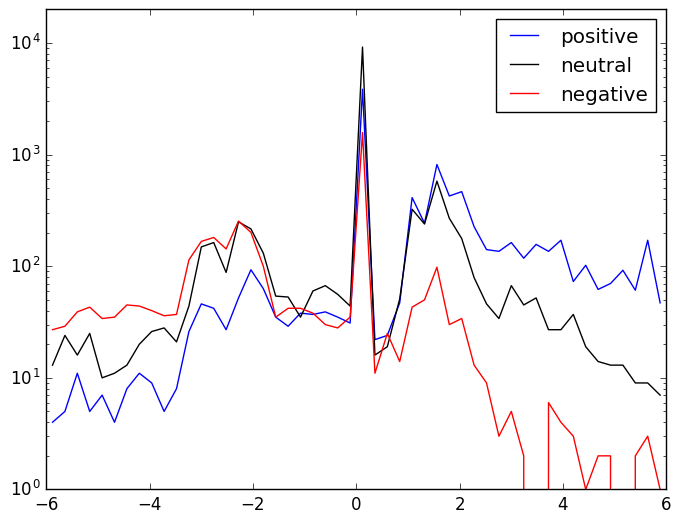
\includegraphics[width=\textwidth]{./figs/distrib/pmi}
        \caption{Histogram for PMI lexicon}
        \label{fig:distrib_pmi}
    \end{subfigure}
    \begin{subfigure}[b]{0.49\textwidth}
        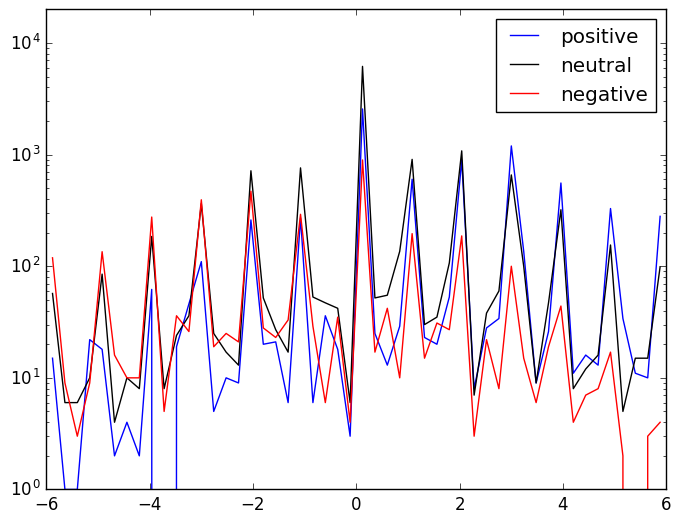
\includegraphics[width=\textwidth]{./figs/distrib/afinn}
        \caption{AFINN lexicon}
        \label{fig:distrib_afinn}
    \end{subfigure}
    \caption{Sentiment value histogram of PMI vs. AFINN Lexicon}
    \label{fig:distrib_comparison}
\end{figure}

Because the comparison of our PMI lexicon and the \textit{AFINN} lexicon is the most reasonable comparison among the three lexica in Table~\ref{tab:lexicon_comparison} a figure visualizing the differences has been created. In Figure~\ref{fig:distrib_comparison} two graphs depicting the distribution of positive, negative and neutral tweets given their sentiment values predicted by our classifier, are shown. In Figure~\ref{fig:distrib_pmi} we can see a clear distinction between the classes. For negative sentiment values, most tweets were negative, second most neutral and least positive. On the other hand, for positive sentiment values, most tweets were positive, second most neutral and least negative. For sentiment values close to zero, neutral tweets are the most common. In Figure~\ref{fig:distrib_afinn}, showing the distribution for the \textit{AFINN} lexicon, we can immediately identify a clear difference from the distribution graph of our PMI lexicon. Where the classes are distinctly separated in the distribution graph for our PMI lexicon, the classes are much closer and overlapping in the distribution graph for the \textit{AFINN} lexicon. One can for the most part identify the same order of classes on both the negative and the positive side, but the distance between them is generally much closer in the distribution graph for the \textit{AFINN} lexicon. The zig-zagged pattern in Figure~\ref{fig:distrib_afinn} is due to \textit{AFINN} lexicon only using integer sentiment values. The separability of the different classes displayed in the graphs shows why our PMI lexicon will generally classify more positive, negative and neutral tweets correctly.


\subsection{Lexicon Classifier in SemEval 2016}
After participating in SemEval 2016 with our Initial Experiment system, we wanted to explore how our lexicon based classifier would affect the final result used as a feature, as well as how it would perform on its own compared to the other participants. \\

\begin{table}[H]
    \centering
    \resizebox{\textwidth}{!}{
    \begin{tabular}{|l|ll|lll|l|l|l|}
    \hline
   & \multicolumn{7}{c|}{\bf F1-Score} & \textbf{Accur.} \\ \cline{2-9}
   & \multicolumn{2}{c|}{\bf 2013} & \multicolumn{3}{c|}{\bf 2014} & \multicolumn{1}{c|}{\bf 2015} & \multicolumn{1}{c|}{\bf 2016} & \multicolumn{1}{c|}{\bf 2016} \\
   \multicolumn{1}{|c|}{\bf System} & \bf Tweet & \bf SMS & \bf Tweet & \bf Tweet & \bf Live- & \bf Tweet & \bf Tweet & \bf Tweet \\
   &  &  & \bf & \bf sarca. & \bf Jour. & & & \\
\hline
NTNUSentEval & 0.623$_{11}$ & 0.641$_{1}$ & 0.651$_{10}$ & 0.427$_{13}$ & 0.719$_{3}$ & 0.599$_{13}$ & \bf 0.583$_{11}$ & 0.643$_{2}$ \\
w/ Lexicon Classifier & 0.648$_{9}$ & 0.659$_{1}$ & 0.667$_{8}$ & 0.438$_{12}$ & 0.707$_{3}$ & 0.609$_{11}$ & \bf 0.583$_{11}$ & 0.636$_{4}$ \\
Lexicon Classifier & 0.597$_{17}$ & 0.565$_{14}$ & 0.614$_{18}$ & 0.284$_{34}$ & 0.590$_{21}$ & 0.554$_{20}$ & \bf 0.541$_{19}$ & 0.603$_{9}$ \\
    \hline
    \end{tabular}}
    \caption[Alternative SemEval 2016 results]{Alternative F1-scores and accuracy results for SemEval 2016 if we had submitted different systems instead. Ordered by F1-scores on the 2016 dataset.}
    \label{tab:alternative_semeval_results}
\end{table}

As shown in Table~\ref{tab:alternative_semeval_results}, using our lexicon based classifier as a feature in our Initial Experiment system \textit{NTNUSentEval}, the F1-score on the 2016 dataset is the same as the score of \textit{NTNUSentEval}. However, on all other datasets except for the Live-Journal dataset, the F1 score is increased, and our placement improved. The performance of our lexicon based classifier on its own is significantly lower, but would still have ended up on 19th place out of the competing 34 systems. 

\subsection{Lexicon Size Comparison}
\label{sec:lexicon_size_comparison}
Another interesting aspect we wanted to explore was how the size of the created sentiment lexicon affected the performance. In order to explore that, eight sentiment lexica of sizes ranging from 500 to 200\thinspace000 entries were created and tested on the four SemEval datasets. \\

\begin{table}[t]
    \centering
    \begin{tabular}{|r|c|c|c|c|}
        \hline
        \textbf{Lexicon Size} & \textbf{2013} & \textbf{2014} & \textbf{2015} & \textbf{2016} \\ \hline
            500                     & 0.3387 & 0.2736 & 0.3029 & 0.3936 \\ \hline
          1\thinspace500            & 0.6533 & 0.6343 & 0.6049 & 0.6016 \\ \hline
      \bf 3\thinspace000            & 0.6748 & 0.6578 & 0.6201 & 0.6032 \\ \hline
         10\thinspace000            & 0.6674 & 0.6507 & 0.6201 & 0.6038 \\ \hline
         25\thinspace000            & 0.6328 & 0.6203 & 0.6020 & 0.6011 \\ \hline
         50\thinspace000            & 0.6052 & 0.6092 & 0.5650 & 0.5976 \\ \hline
        100\thinspace000            & 0.6040 & 0.6090 & 0.5648 & 0.5851 \\ \hline
        200\thinspace000            & 0.5965 & 0.6020 & 0.5626 & 0.5938 \\ \hline
    \end{tabular}
    \caption[Comparison of different sized PMI lexica]{Comparison of different sized PMI lexica after being tested on the 2013-2016 SemEval datasets.}
    \label{tab:comparison_different_size_lexica}   
\end{table}

As we can see from Table~\ref{tab:comparison_different_size_lexica}, as long as the lexicon size is above a certain threshold, the overall performance remain acceptable. We do, however, see a continuous drop in performance when the lexicon size passes 10\thinspace000 entries. \\

The best performing lexicon from the above test, has 3\thinspace000 entries, which is quite interesting looking at the \textit{Sentiment140} lexicon with approximately 300\thinspace000 entries in comparison. More words and phrases do not necessary lead to better results. Although that statement is valid for our lexicon creation approach, no general conclusion can be drawn. Our lexicon creation process as described in Section~\ref{sec:pmi_lexicon_creation}, only includes vocabulary entries also found in the \textit{Labeled} dataset containing $6.25$ million labeled tweets. Although the size of the \textit{Labeled} dataset is large enough, and its contents are mostly classified correctly, many relevant words and phrases might not have been included. Since the \textit{Labeled} dataset is created, as described in Section~\ref{sec:labeled}, using the \textit{AFINN} lexicon and an inclusion threshold of absolute sentiment value, both tweets with few positive and negative words, and positive and negative tweets with only a few words found in \textit{AFINN} are left out. A better method of creating a labeled dataset might therefore be the solution to create larger lexica with better performance. \\

In addition to the F1-score of the different sized lexica, we also wanted to see the difference in coverage between them. In terms of coverage, four different measures were used: 
\begin{itemize}
    \item \textbf{NZS} (Tweets with Non-Zero Sentiment): Ratio of tweets where final predicted sentiment value was $\neq 0$.
    \item \textbf{TwM} (Tweets with Multi-grams): Ratio of tweets that included at least one multi-gram from the lexicon.
    \item \textbf{WiL} (Words in Lexicon): Ratio of words in tweets found in the lexicon.
    \item \textbf{FWiL} (Frequent Words in Lexicon): Ratio of top 1\thinspace000 most common, non-stop-word words found in the lexicon.
\end{itemize}  

\begin{table}[t]
    \centering
    \begin{tabular}{|r|c|c|c|c|}
        \hline
        \textbf{Lexicon Size} & \textbf{NZS} & \textbf{TwM} & \textbf{WiL} & \textbf{FWiL} \\ \hline
            500                     & 0.0435 & 0.0066 & 0.3567 & 0.0081 \\ \hline
          1\thinspace500            & 0.3902 & 0.0086 & 0.3793 & 0.0655 \\ \hline
      \bf 3\thinspace000            & 0.4726 & 0.0412 & 0.3632 & 0.0826 \\ \hline
         10\thinspace000            & 0.4922 & 0.0702 & 0.3647 & 0.0846 \\ \hline
         25\thinspace000            & 0.8421 & 0.1788 & 0.4012 & 0.1712 \\ \hline
         50\thinspace000            & 0.9968 & 0.3322 & 0.5229 & 0.4371 \\ \hline
        100\thinspace000            & 0.9992 & 0.4703 & 0.6122 & 0.7019 \\ \hline
        200\thinspace000            & 0.9996 & 0.6012 & 0.6692 & 0.9889 \\ \hline
    \end{tabular}
    \caption{Lexicon coverage overview}
    \label{tab:lexicon_coverage}   
\end{table}

From Table~\ref{tab:lexicon_coverage} the results of our coverage experiment are shown. Interestingly the best performing lexicon with a size of 3\thinspace000 only contains words found in $47\%$ of the tweets. That means, that almost half of the tweets end up with a sentiment score of zero and are classified as neutral. In addition only approximately $4\%$ of the tweets contain multi-grams ($n$-grams with $n>2$) found in the lexicon, which in turn means that parts of our lexicon are never used. Although the scores for the different coverage measures increase with the lexicon size, meaning larger lexicon lead to higher coverage, it does not look like higher coverage means better classification performance. As discussed previously in this section, we also believe this is caused by our \textit{Labeled} dataset, that would both need to be larger and include a more varied language with more words and phrases. \\

\begin{figure}[t]
    \centering
    \begin{subfigure}[b]{0.49\textwidth}
        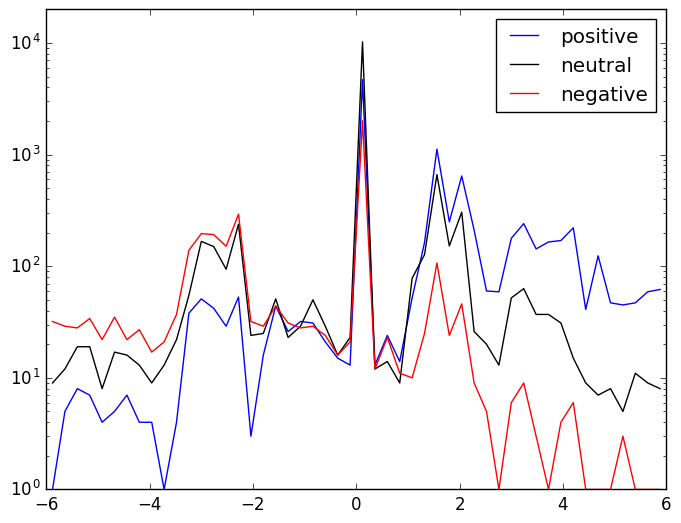
\includegraphics[width=\textwidth]{./figs/distrib/1500}
        \caption{Histogram for PMI lexicon, size 1\thinspace500}
        \label{fig:distrib_1500}
    \end{subfigure}
    \begin{subfigure}[b]{0.49\textwidth}
        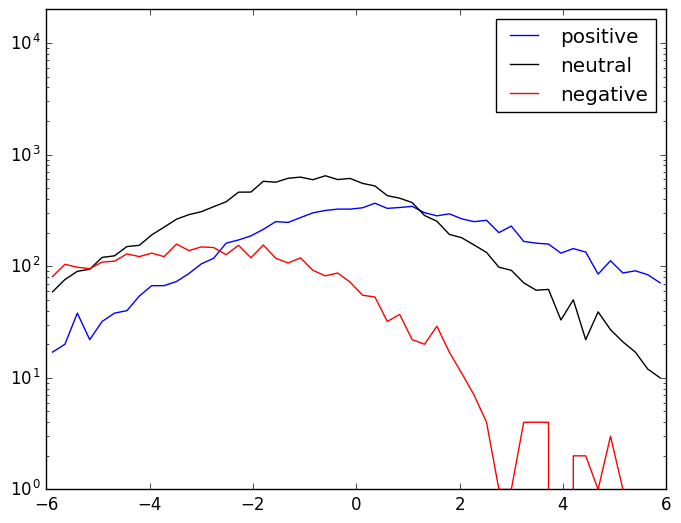
\includegraphics[width=\textwidth]{./figs/distrib/200000}
        \caption{Histogram for PMI lexicon, size 200\thinspace000}
        \label{fig:distrib_200000}
    \end{subfigure}
    \caption{Sentiment value histogram of small vs. large PMI Lexicon}
    \label{fig:distrib_size_comparison}
\end{figure}

Figure~\ref{fig:distrib_size_comparison} shows the distribution of positive, negative and neutral tweets given their sentiment value predicted by our classifier on a PMI lexicon of size 1\thinspace500 and of size 200\thinspace000. In comparison to Figure~\ref{fig:distrib_pmi}, showing the same distribution for our best PMI lexicon, the difference in performance is even further visualized. Compared to the distribution of our best PMI lexicon, the distribution of the 200\thinspace000 lexicon, shown in Figure~\ref{fig:distrib_200000} is almost an uniform distribution, the large spike around 0 is gone, but the differences between classes are smaller. The other extreme is the distribution of the small lexicon, shown in Figure~\ref{fig:distrib_1500}. It classifies some of the positive and negative tweets well, but most tweets are left with a score of 0.

\section{Best Performing PMI Lexicon}
After identifying our best performing PMI lexicon, a few statistics were gather in order to see whether or not the resulting lexicon contained the features we expected. It also provides a general insight into the lexicon created. \\

\begin{table}[t]
    \begin{tabular}{| l | l || l | l |}
        \hline
        \multicolumn{2}{|c||}{\textbf{Positive}} & \multicolumn{2}{c|}{\textbf{Negative}} \\ \hline
        \textbf{$n$-gram} & \textbf{Value} & \textbf{$n$-gram} & \textbf{Value} \\ \hline
        you have a great day        & 5.00 & a bad bitch        & -5.00 \\ \hline
        you have an amazing day     & 4.48 & bitch ass nigga    & -4.95 \\ \hline
        hope its a good one         & 4.33 & dumb ass           & -4.82 \\ \hline
        happy birthday i hope       & 4.21 & fuck that bitch    & -4.75 \\ \hline
        you had a great day         & 4.10 & fuck a bitch       & -4.75 \\ \hline
        you have a good day         & 4.08 & bad right now      & -4.73 \\ \hline
        you have a wonderful day    & 4.02 & weak ass           & -4.72 \\ \hline
        hope you have a great       & 4.01 & fuck this shit     & -4.68 \\ \hline
        you have a good one         & 3.99 & fuck fuck fuck     & -4.66 \\ \hline
        i love love love            & 3.96 & fool me twice      & -4.63 \\ \hline
    \end{tabular}
    \caption[Top 10 positive and negative entries in our lexicon]{The top 10 positive and negative entries in our best performing lexicon}
    \label{tab:lexicon_ngram_entries}
\end{table}

From Table~\ref{tab:lexicon_ngram_entries}, where the top 10 positive and negative lexicon entries are listed, we can clearly identify all of the top 10 positive as actual positive phrases and the top 10 negative as negative phrases. In addition we do not see any unigrams, meaning that our attempt of scoring longer $n$-grams higher/lower than shorter $n$-grams seems to be working.  \\

\begin{table}[t]
    \begin{tabular}{| c | l | l || c | l | l |}
        \hline
        \multicolumn{3}{|c||}{\textbf{Positive}} & \multicolumn{3}{c|}{\textbf{Negative}} \\ \hline
        \textbf{Emoji} & \textbf{Alias} & \textbf{Value} & \textbf{Emoji} & \textbf{Alias} & \textbf{Value} \\ \hline
        
\includegraphics[height=.5cm]{./figs/emojis/birthday} & Birthday Cake & 2.76 
        & 
\includegraphics[height=.5cm]{./figs/emojis/rage} & Pouting Face & -2.64 \\ \hline
        
\includegraphics[height=.5cm]{./figs/emojis/gift} & Wrapped Present & 2.60 
        & 
\includegraphics[height=.5cm]{./figs/emojis/parking} & Parking Sign & -2.41 \\ \hline
        
\includegraphics[height=.5cm]{./figs/emojis/balloon} & Balloon & 2.51 
        & 
\includegraphics[height=.5cm]{./figs/emojis/angry} & Angry Face & -2.41 \\ \hline
        
\includegraphics[height=.5cm]{./figs/emojis/confetti_ball} & Confetti Ball & 2.47 
        & 
\includegraphics[height=.5cm]{./figs/emojis/triumph} & Triumph Face & -2.40 \\ \hline
        
\includegraphics[height=.5cm]{./figs/emojis/party_popper} & Party Popper & 2.46 
        & 
\includegraphics[height=.5cm]{./figs/emojis/put_litter_in_its_place} & Litterbox & -2.34 \\ \hline
    \end{tabular}
    \caption[Top 5 positive and negative emojis in our lexicon]{The top 5 positive and negative emojis in our best performing lexicon}
    \label{tab:lexicon_emoji_entries}
\end{table}

Just like positive and negative phrases were separated with opposite sentiment values, the detected emojis were treated the same way, as seen in Table~\ref{tab:lexicon_emoji_entries}. All emojis listed as positive are commonly used to further express positive sentiment in positive sentences, while all of the emojis listed as negative are commonly used in negative sentences. \\

\begin{table}[t]
    \centering
    \begin{tabular}{| l | c |}
    \hline
    \textbf{$n$-gram} & \textbf{Value} \\ \hline
    you have a great day & 5.00  \\ \hline
    have a great day &  3.54 \\ \hline
    a great day & 2.16 \\ \hline
    great & 2.04 \\ \hline
    \end{tabular}
    \caption[Effect of $n$-gram length on sentiment value in our lexicon]{The effect of $n$-gram length on sentiment value}
    \label{tab:lexicon_entry_length_effect}
\end{table}

As mentioned earlier in this section, we wanted to create a lexicon where a long $n$-gram containing a polarized word should get a higher absolute sentiment value than a shorter $n$-gram containing the same word. In Table~\ref{tab:lexicon_entry_length_effect} this feature is identified through the four listed phrases containing the polarized word "great".

\section{Labeled Dataset Size Comparison}
\label{sec:labeled_dataset_size_comparison}
To better understand the relationship between the size of the labeled dataset and the performance of the resulting lexicon, we performed an experiment where we created lexica using different sized subsets of our \textit{Labeled} dataset. \\

\begin{table}[t]
    \centering
    \begin{tabular}{|r|c|c|c|c|}
        \hline
        \textbf{Labeled Size} & \textbf{2013} & \textbf{2014} & \textbf{2015} & \textbf{2016} \\ \hline
            50\thinspace000                 & 0.6002 & 0.5897 & 0.5584 & 0.5635 \\ \hline
            100\thinspace000                & 0.6262 & 0.6136 & 0.5830 & 0.5722 \\ \hline
            500\thinspace000                & 0.6601 & 0.6447 & 0.6142 & 0.5984 \\ \hline
            1\thinspace000\thinspace000     & 0.6686 & 0.6541 & 0.6130 & 0.6046 \\ \hline
            3\thinspace000\thinspace000     & 0.6677 & 0.6512 & 0.6153 & 0.6052 \\ \hline
            \bf 6\thinspace250\thinspace000 & 0.6748 & 0.6578 & 0.6201 & 0.6032 \\ \hline
    \end{tabular}
    \caption[Comparison of different sized labeled dataset]{Comparison of different sized labeled dataset after being tested on the 2013-2016 SemEval datasets.}
    \label{tab:labeled_size_comparison}   
\end{table}

Table~\ref{tab:labeled_size_comparison} shows the result of the experiment. The size of the labeled dataset seems to matter a lot at the beginning, but it quickly reaches a state where additional tweets provide almost no new information. This could be an artifact of the labeled dataset set creation method, since it includes only tweets containing words found in the \textit{AFINN} lexicon.


\section{Ablation Study}
\label{sec:ablation_study_lexicon_classifier}
To detect the impact each feature of both our lexicon creator and classifier impose on the performance, an ablation study was conducted. This was done by removing each feature in turn to see how the removal affected the system performance. Since our system, a lexicon based classifier using a PMI lexicon, is affected both by features used in the classification process and by features used in the creation process, the ablation study involved removing features from both processes. \\


\begin{table}[t]
    \centering
    \begin{tabular}{|l|c|c|c|c|}
        \hline
        \textbf{Features} & \textbf{2013} & \textbf{2014} & \textbf{2015} & \textbf{2016} \\ \hline
        All                         & 0.6748 & 0.6578 & 0.6201 & 0.6032 \\ \hline
        All - Adjectives/Adverbs    & 0.6653 & 0.6525 & 0.6127 & 0.6032 \\ \hline
        All - Negation              & 0.6732 & 0.6561 & 0.6180 & 0.6030 \\ \hline
        All - Intensification       & 0.6733 & 0.6548 & 0.6193 & 0.6036 \\ \hline
        All - PMI $n$-grams         & 0.6714 & 0.6503 & 0.6161 & 0.6010 \\ \hline
    \end{tabular}
    \caption[Ablation study results for lexicon classifier]{Ablation study results. All - F means all features except for F. All values are $F_1$-scores. The datasets used are the 2013-2016 SemEval datasets.}
    \label{tab:ablation_study_lexicon_classifier}   
\end{table}

As we can see from Table~\ref{tab:ablation_study_lexicon_classifier}, the impact each feature imposes on the performance of our classifier is very subtle, with the single most important feature being the adjective and adverb addition which increases the F1-score on the 2013 dataset by $0.01$. This means that the performance of our classifier almost entirely relies on the quality of our PMI lexicon, with the additional features only contributing a small amount. The second most important feature is our PMI $n$-grams used in the lexicon creation process. When replacing the PMI $n$-grams with frequency $n$-grams, $n$-grams selected solely based on their frequency, the F1-score drops by $0.0075$ on the 2014 dataset. Although we do see an improvement when using PMI $n$-grams over frequency $n$-grams, the small impact it has surprised us. By looking at the resulting lexica using the two $n$-gram approaches, the lexicon created with PMI $n$-grams looks far more promising than the lexicon created with frequency $n$-grams. \\

The small impact of negation and intensification is also somewhat surprising. While our lexicon excludes any $n$-gram containing intensifiers, negators are allowed. This is to better deal with common phrases containing negation, for example \textit{"glad im not the only one"} is an actual phrase included in one of our lexica, and its sentiment value is positive. Therefore some of the common negated phrases are already included in the lexicon and simply turning off the negation detection inside the classifier will only have an effect on less common phrases. The small effect of intensifiers is due to their low frequency, less than 1\% of the tweets contained any intensifiers.

\glsresetall


%!TEX root = ../report.tex
\chapter{Discussion}
\label{cha:discussion}
In this chapter we evaluate our accomplishments, draw conclusions based on the conducted experiments and suggest possible future work. 

\section{Evaluation}
\label{sec:evaluation}
During the initial phase of this Master's Thesis work, four goals were formulated and described in Section~\ref{sec:project_goals}. In this section we evaluate to which degree each goal has been accomplished and discuss the overall quality of the developed systems. 

\subsection*{G1: Research Automatic Creation of Sentiment Lexica}
The field of automatic creation of sentiment lexica has been explored, in search of the most commonly used and best performing approaches. The research resulted in the identification of two main approaches: a graph approach and a \ac{pmi} approach. The information gathered and the knowledge gained in the field formed the basis for our work with our third goal (G3). 

\subsection*{G2: Research Lexicon Based Sentiment Analysis}
In addition to the research done to reach our first goal, we also studied the field of lexicon based \ac{sa}. Although the use of sentiment lexica is widespread within the field of \ac{sa}, we found that most \ac{sa} systems only use sentiment lexica as a feature among a series of features instead of basing the system around them which was what we wanted to explore. We were, however, able to identify interesting ideas and methods from the few lexicon based \ac{sa} systems we discovered. In addition to the more common uses of sentiment lexica within \ac{sa}, the ideas and methods from the lexicon based systems acted as a basis for the work on our fourth goal (G4).  

\subsection*{G3: Create a Twitter Specific Sentiment Lexicon}
By developing a sentiment lexica creator utilizing the core \ac{pmi} approach discovered in our research, a Twitter specific sentiment lexicon was successfully created. After two months of experimenting with a graph propagation approach without satisfactory results, we decided to try out the \ac{pmi} approach which instantly yielded better results, as described in Section~\ref{sec:transition_graph_pmi} and shown in Table~\ref{tab:graph_vs_pmi}. From that point on, the lexicon creator utilizing the \ac{pmi} approach became our main focus regarding the task of sentiment lexica creation. \\

The best performing sentiment lexicon we were able to create with our sentiment lexica creator, was a lexicon with 3\thinspace000 entries consisting of $n$-grams with $n\leq5$ selected based on their \ac{pmi} score and occurrence frequency. Compared to the previously created sentiment lexica, \textit{Sentiment140} and \textit{AFINN}, our lexicon seemingly outperforms the other two, as shown in Table~\ref{tab:lexicon_comparison}. However, as described in Section~\ref{sec:lexicon_comparison}, because our system is unable to utilize all features of the \textit{Sentiment140} lexicon no clear conclusion can be drawn based on the results. The performance of our lexicon against the \textit{AFINN} lexicon on the other hand is a more valid comparison. The fact that our lexicon outperforms the \textit{AFINN} lexicon, which is a commonly used manually annotated sentiment lexicon within \ac{sa}, shows that the overall quality of our lexicon is high.  

\subsection*{G4: Create a Lexicon Based Sentiment Analysis System}
A lexicon based sentiment analysis system/lexicon based classifier has been created. The classifier was developed in parallel with our lexicon creator, and is therefore specifically tailored to work well with our sentiment lexicon. Through the results of the performance tests described in Section~\ref{sec:system_performance}, we can see that the classifier utilizing our best performing sentiment lexicon almost keeps up with the two best performing comparison systems, the system by \citeauthor{FaretReitan} and the Initial Experiment, both utilizing \ac{svm} in the classification process. While achieving such good results, regarding F1-score, recall and precision our lexicon classifier completely outperforms the other systems in terms of run-time performance which along with the other performance measures has been a focus area throughout the development process. \\

When utilized as a feature in our Initial Experiment system we see a significant boost in performance. The classifier proves that its able to provide the \ac{svm} in our Initial Experiment system with additional and relevant information, further verifying its overall quality. As discovered in the ablation study described in Section~\ref{sec:ablation_study_lexicon_classifier}, the performance of the classifier is highly dependent on the quality of the lexicon it uses, and not so much on its different features. Good results for our classifier therefore also point to a high quality sentiment lexica.


\section{Conclusion}
\label{sec:conclusion}
Through the various experiments described in Section~\ref{sec:system_performance} we have discovered that the \ac{pmi} lexicon creation approach works well, but that the quality of the created lexicon is highly dependent on the quality of the large labeled tweet dataset. Acquiring a large labeled dataset of high quality, that is, a diverse dataset capturing as many aspects of the language as possible, is a difficult task. From our experiment of comparing different sized labeled datasets, described in Section~\ref{sec:labeled_dataset_size_comparison}, we see that once the dataset reaches a certain size, the performance of the resulting lexicon reaches its maximum only limited by the quality of the dataset. By using the \textit{AFINN} lexicon, the labeled dataset is limited to contain tweets with words and phrases found in the lexicon. Possible new and interesting lexicon words or phrases will only be found if they happen to also be part of a tweet containing enough words in \textit{AFINN}. \\

Another interesting result further supporting the \ac{pmi} lexicon creation approach and the quality of our lexicon and lexicon classifier, is the lexicon comparison results described in Section~\ref{sec:lexicon_comparison}. Our fully automatically created \ac{pmi} lexicon actually beats the manually annotated \textit{AFINN} lexicon on all datasets across all performance measures, which is both an important result and a noticeable feat. In addition to verifying the quality of our lexicon it also proves that creating sentiment lexica automatically is a highly viable sentiment lexicon creation method. \\

Throughout the development process of our lexicon creation system and our lexicon based classifier, as well as through the various experiments conducted in Chapter~\ref{cha:experiments}, the tight connection between the sentiment lexicon and the system utilizing the lexicon has become apparent. For a classifier to utilize a sentiment lexicon's full potential, the classifier must be specifically tailored to work with that specific lexicon. This is a consequence of the different sentiment lexica creation methods, where the creators of the different available lexica apply different features to their lexicon specifically meant to work well in another system or classifier. That is, there is no standardized format for automatically created sentiment lexica. \\

Based on our initial research within the field of automatic creation of sentiment lexica, we assumed that one of the feats of automatically created sentiment lexica would be that their size and word coverage would benefit their performance compared to manually annotated lexica. However, after our experiments of comparing lexica of various sizes, described in Section~\ref{sec:lexicon_size_comparison}, our assumption was not verified. Larger lexica did lead to a better coverage as shown in Table~\ref{tab:lexicon_coverage}, but their classification performance was not improved accordingly. Although our results point to that larger lexica with high coverage would not perform better than relatively small lexica with medium coverage, no definite conclusions can be drawn. The fact that larger lexica created with our lexicon creator did not lead to better performance might also be caused by the quality of the labeled dataset used, described earlier in this section. \\

Regarding the run-time performance of lexicon based \ac{sa} systems compared to more sophisticated \ac{sa} systems, our results clearly suggest that lexicon based systems are the most viable \ac{sa} systems to use in real-time classification applications. With our lexicon based classifier, we achieve a classification speed of 108\thinspace600 tweets per second, meaning that our system could have classified all of the 500 million tweets posted on Twitter each day in real-time 19 times over. With this result it would be possible to add more advanced features to our classifier, trading off run-time performance for better classification performance and still classify fast enough to be a real-time classifier.


\section{Future Work}
\label{sec:future_work}
Throughout the work on this Master's Thesis, a series of possible improvements for our developed systems along with other future work have been discovered. \\

\subsection{Multidimensional Lexicon}
The source of most of our misclassifications are the tweets with sentiment value of 0. In our current implementation, all these tweets are classified as neutral by default. We think it should be possible to extract several other values for each $n$-gram to the lexicon that can actually help classify a tweet as neutral instead of classifying all tweets with sentiment value of 0 as neutral. For example, each word could have a sentiment score and an objectivity score. The sentiment score would be calculated as it is today, while the objectivity score would be calculated also using the PMI approach, but on a dataset labeled as subjective/objective. 

\subsection{PMI approach}
When counting the positive and negative contexts for an $n$-gram in our \ac{pmi} approach to lexicon creation, negation is not handled. That is, if a tweet as a whole is labeled as positive, but there exists negated $n$-grams within the tweet, we still increment the positive context counter of the $n$-grams. However, we believe that the performance of the final lexicon might benefit from handling the negated $n$-grams differently in this counting process. This can be done by, for example, incrementing the opposite context counter or perhaps by incrementing the context counter by a smaller amount if the $n$-gram is negated. \\

\subsection{Graph Approach}
Because our main focus changed from the graph propagation approach to the \ac{pmi} approach for lexicon creation, some of the more advanced features or improvements of the \ac{pmi} lexicon were never incorporated into the graph propagation approach. It would therefore be interesting to see how and if \ac{pmi} $n$-grams, as opposed to the occurrence frequency $n$-grams we used, affect the overall performance of the graph propagation approach.\\

Another, perhaps more important improvement is how the similarity between the different context vectors is calculated. In our approach, the similarity measure cosine similarity is used. However, the similarity measure we believe would work best is the Pearson Correlation similarity measure, which is the fourth and final step in the COALS method where we only follow the first three. \\

\subsection{Combined Approach}
Where the \ac{pmi} lexicon creation approach is only concerned with finding the sentiment values of $n$-grams, the graph propagation approach is most concerned with the relationship between the different $n$-grams. The graph propagation approach namely strives to find similar $n$-grams. That is, $n$-grams used in similar contexts. Because one of the problems of the graph propagation approach is to find a good seed set with appropriate weights, it could be interesting to explore a lexicon creation system combining the \ac{pmi} approach and the graph propagation approach. The \ac{pmi}-approach could be used to identify a seed set with sentiment values, while the graph propagation approach could be used to find $n$-grams similar to the ones already present in the seed set. With more appropriate seed set values, the most similar $n$-grams found during graph propagation would hopefully be assigned more appropriate sentiment values themselves. \\ 

\subsection{Lexicon Extension}
Another interesting possible improvement is to extend the adjective and adverb addition. In addition to deriving the adverb and the missing forms of an adjective, one can explore the possibilities of adding the different forms of verbs. The verb \textit{love} for example, has the forms \textit{loves}, \textit{loved} and \textit{loving}, which could possibly be added to a lexicon if not already present. Exploring how to set the sentiment values of the missing verb forms would then also need to be done. One possible approach would be to set the sentiment value of a missing word to the initial word already found in the lexicon, but only add words if the initial word has an absolute sentiment value above a set threshold. \\

A different approach entirely could be to use a synonym dictionary. That way, synonyms of words already found in the lexicon could be added to expand and hopefully improve the overall coverage of the lexicon. The synonyms found could be given the same sentiment value as their related $n$-gram. This approach in combination with the aforementioned approach could be especially interesting.\\

\subsection{Lexicon Based Classifier}
Regarding our lexicon based classifier, there are three features in particular we believe would be interesting to explore further: capitalized words, elongated words and more special weights on non-letter characters. In our classifier all tweets are transformed into lower-case, disregarding all capitalized words. Exploring how one can utilize the use of capitalized words in a lexicon based classifier would therefore be interesting. \\

Although almost all elongated words are corrected, the fact that a word indeed was elongated is not utilized in the classification process. Similarly to the capitalized words, elongated words are also often used to boost sentiment value. A possible approach to utilizing the use of elongation could be to multiply the sentiment value of the corrected elongated word as a function of excess repeated characters in the word. \\

Almost all non-letter characters except "!" and "?" are removed in our system. Looking into such as the use of quotation and repeated use of the punctuation character "." and how they might affect the overall sentiment could also be particularly valuable. 

\glsresetall

\addcontentsline{toc}{chapter}{Bibliography}

\bibliographystyle{plainnat}
\bibliography{bib/bibliography}

% alternative, if using biber as backend
% \printbibliography

%!TEX root = ../report.tex
\appendix

%!TEX root = ../report.tex
\chapter{Special Words}
\label{apx:special_words}


\section{Stopwords}
\begin{table}[H]
    \begin{tabular}{| l | l | l | l | l | l | l |}
        \hline
        \multicolumn{7}{|c|}{\textbf{Stopwords}} \\ \hline
        a & about & above & after & again & against & all \\ \hline
        am & an & and & any & are & arent & as \\ \hline
        at & be & because & been & before & being & below \\ \hline
        between & both & but & by & cant & cannot & could \\ \hline
        couldnt & did & didnt & do & does & doesnt & doing \\ \hline
        dont & down & during & each & few & for & from \\ \hline
        further & had & hadnt & has & hasnt & have & havent \\ \hline
        having & he & hed & hell & hes & her & here \\ \hline
        heres & hers & herself & him & himself & his & how \\ \hline
        hows & i & id & ill & im & ive & if \\ \hline
        in & into & is & isnt & it & its & its \\ \hline
        itself & lets & me & more & most & mustnt & my \\ \hline
        myself & no & nor & not & of & off & on \\ \hline
        once & only & or & other & ought & our & ours \\ \hline
        ourselves & out & over & own & same & shant & she \\ \hline
        shed & shell & shes & should & shouldnt & so & some\\ \hline
        such & than & that & thats & the & their & theirs\\ \hline
        them & themselves & then & there & theres & these & they\\ \hline
        theyd & theyll & theyre & theyve & this & those & through\\ \hline
        to & too & u & under & until & up & ur\\ \hline
        ure & very & was & wasnt & we & wed & well\\ \hline
        were & weve & were & werent & what & whats & when\\ \hline
        whens & where & wheres & which & while & who & whos\\ \hline
        whom & why & whys & with & wont & would & wouldnt\\ \hline
        you & youd & youll & youre & youve & your & yours\\ \hline
        yourself & yourselves & \multicolumn{5}{c|}{} \\ \hline
    \end{tabular}
    \caption[List of all stopwords used in our lexicon based system]{List of all stopwords used in our lexicon creators and lexicon based classifier. Consists of stopwords collected from \textit{http://www.ranks.nl/stopwords}.}
    \label{tab:master_stopwords}
\end{table}


\section{Negation cues}
\begin{table}[H]
    \begin{tabular}{| l | l | l | l | l | l | l |}
        \hline
        \multicolumn{7}{|c|}{\textbf{Negation Cues}} \\ \hline
        aint & anit & cant & cannot & couldnt & didnt & dnt \\ \hline
        doesnt & dont & dont & hadnt & hasnt & havent & havnt \\ \hline
        isnt & lack & lacking & lacks & never & no & nor \\ \hline
        not & shouldnt & wasnt & wont & wouldnt & \multicolumn{2}{c|}{} \\ \hline
    \end{tabular}
    \caption{List of all negation cues used in our lexicon based system}
    \label{tab:master_negation_cues}
\end{table}


\section{Intensifiers}
\begin{table}[H]
    \centering
    \begin{tabular}{| l | l || l | l || l | l |}
        \hline
        \textbf{Modifier} & \textbf{Weight} & \textbf{Modifier} & \textbf{Weight} & \textbf{Modifier} & \textbf{Weight}\\ \hline
        most & 2.00         & very & 1.25           & kinda & 0.80      \\ \hline
        incredibly & 1.80   & completely & 1.20     & sort of & 0.80    \\ \hline
        extremely & 1.70    & hella & 1.20          & sorta & 0.80      \\ \hline
        absolutely & 1.50   & more & 1.20           & somewhat & 0.70   \\ \hline
        fucking & 1.40      & particularly & 1.20   & hardly & 0.70     \\ \hline
        totally & 1.30      & so & 1.20             & barely & 0.60     \\ \hline
        greatly & 1.25      & quite & 1.10          & slightly & 0.50   \\ \hline
        highly & 1.25       & pretty & 0.90         & \multicolumn{2}{c|}{} \\ \hline
        really & 1.25       & kind of & 0.80        & \multicolumn{2}{c|}{} \\ \hline
    \end{tabular}
    \caption[List of all intensifiers used in our lexicon based system]{List of all intensifiers used in our lexicon creators and lexicon based classifier. Consists of a subset of intensifiers used in the \textit{VADER Sentiment} system by \cite{vaderSentiment}}
    \label{tab:intensifiers}
\end{table} 


%!TEX root = ../report.tex
\chapter{SemEval 2016 Results}
\label{apx:semeval_results}

\begin{table}[H]
    \centering
    \resizebox{\textwidth}{!}{
    \begin{tabular}{|l|ll|lll|l|l|l|}
    \hline
   & \multicolumn{7}{c|}{\bf F1-Score} & \textbf{Accur.} \\ \cline{2-9}
   & \multicolumn{2}{c|}{\bf 2013} & \multicolumn{3}{c|}{\bf 2014} & \multicolumn{1}{c|}{\bf 2015} & \multicolumn{1}{c|}{\bf 2016} & \multicolumn{1}{c|}{\bf 2016} \\
   \multicolumn{1}{|c|}{\bf System} & \bf Tweet & \bf SMS & \bf Tweet & \bf Tweet & \bf Live- & \bf Tweet & \bf Tweet & \bf Tweet \\
   &  &  & \bf & \bf sarca. & \bf Jour. & & & \\
\hline
SwissCheese & 0.700$_{4}$ & 0.637$_{2}$ & 0.716$_{4}$ & 0.566$_{1}$ & 0.695$_{7}$ & 0.671$_{1}$ & \bf 0.633$_{1}$ & 0.646$_{1}$ \\
SENSEI-LIF & 0.706$_{3}$ & 0.634$_{3}$ & 0.744$_{1}$ & 0.467$_{8}$ & 0.741$_{1}$ & 0.662$_{2}$ & \bf 0.630$_{2}$ & 0.617$_{7}$ \\
unimelb & 0.687$_{6}$ & 0.593$_{9}$ & 0.706$_{6}$ & 0.449$_{11}$ & 0.683$_{9}$ & 0.651$_{4}$ & \bf 0.617$_{3}$ & 0.616$_{8}$ \\
INESC-ID & 0.723$_{1}$ & 0.609$_{6}$ & 0.727$_{2}$ & 0.554$_{2}$ & 0.702$_{4}$ & 0.657$_{3}$ & \bf 0.610$_{4}$ & 0.600$_{10}$ \\
aueb.twitter.sent.. & 0.666$_{7}$ & 0.618$_{5}$ & 0.708$_{5}$ & 0.410$_{17}$ & 0.695$_{7}$ & 0.623$_{7}$ & \bf 0.605$_{5}$ & 0.629$_{6}$ \\
SentiSys & 0.714$_{2}$ & 0.633$_{4}$ & 0.723$_{3}$ & 0.515$_{4}$ & 0.726$_{2}$ & 0.644$_{5}$ & \bf 0.598$_{6}$ & 0.609$_{9}$ \\
I2RNTU & 0.693$_{5}$ & 0.597$_{7}$ & 0.680$_{7}$ & 0.469$_{6}$ & 0.696$_{6}$ & 0.638$_{6}$ & \bf 0.596$_{7}$ & 0.593$_{12}$ \\
INSIGHT-1 & 0.602$_{16}$ & 0.582$_{12}$ & 0.644$_{15}$ & 0.391$_{23}$ & 0.559$_{23}$ & 0.595$_{16}$ & \bf 0.593$_{8}$ & 0.635$_{5}$ \\
twise & 0.610$_{15}$ & 0.540$_{16}$ & 0.645$_{13}$ & 0.450$_{10}$ & 0.649$_{13}$ & 0.621$_{8}$ & \bf 0.586$_{9}$ & 0.528$_{24}$ \\
ECNU & 0.643$_{9}$ & 0.593$_{9}$ & 0.662$_{8}$ & 0.425$_{14}$ & 0.663$_{10}$ & 0.606$_{11}$ & \bf 0.585$_{10}$ & 0.571$_{16}$ \\
\bf NTNUSentEval & 0.623$_{11}$ & 0.641$_{1}$ & 0.651$_{10}$ & 0.427$_{13}$ & 0.719$_{3}$ & 0.599$_{13}$ & \bf 0.583$_{11}$ & 0.643$_{2}$ \\
MDSENT & 0.589$_{19}$ & 0.509$_{20}$ & 0.587$_{20}$ & 0.386$_{24}$ & 0.606$_{18}$ & 0.593$_{17}$ & \bf 0.580$_{12}$ & 0.545$_{20}$ \\
CUFE & 0.642$_{10}$ & 0.596$_{8}$ & 0.662$_{8}$ & 0.466$_{9}$ & 0.697$_{5}$ & 0.598$_{14}$ & \bf 0.580$_{12}$ & 0.637$_{4}$ \\
THUIR & 0.616$_{12}$ & 0.575$_{14}$ & 0.648$_{11}$ & 0.399$_{20}$ & 0.640$_{15}$ & 0.617$_{10}$ & \bf 0.576$_{14}$ & 0.596$_{11}$ \\
PUT & 0.565$_{21}$ & 0.511$_{19}$ & 0.614$_{19}$ & 0.360$_{27}$ & 0.648$_{14}$ & 0.597$_{15}$ & \bf 0.576$_{14}$ & 0.584$_{14}$ \\
LYS & 0.650$_{8}$ & 0.579$_{13}$ & 0.647$_{12}$ & 0.407$_{18}$ & 0.655$_{11}$ & 0.603$_{12}$ & \bf 0.575$_{16}$ & 0.585$_{13}$ \\
IIP & 0.598$_{17}$ & 0.465$_{23}$ & 0.645$_{13}$ & 0.405$_{19}$ & 0.640$_{15}$ & 0.619$_{9}$ & \bf 0.574$_{17}$ & 0.537$_{23}$ \\
UniPI & 0.592$_{18}$ & 0.585$_{11}$ & 0.627$_{17}$ & 0.381$_{25}$ & 0.654$_{12}$ & 0.586$_{18}$ & \bf 0.571$_{18}$ & 0.639$_{3}$ \\
DIEGOLab16 & 0.611$_{14}$ & 0.506$_{21}$ & 0.618$_{18}$ & 0.497$_{5}$ & 0.594$_{20}$ & 0.584$_{19}$ & \bf 0.554$_{19}$ & 0.549$_{19}$ \\
GTI & 0.612$_{13}$ & 0.524$_{17}$ & 0.639$_{16}$ & 0.468$_{7}$ & 0.623$_{17}$ & 0.584$_{19}$ & \bf 0.539$_{20}$ & 0.518$_{26}$ \\
OPAL & 0.567$_{20}$ & 0.562$_{15}$ & 0.556$_{23}$ & 0.395$_{21}$ & 0.593$_{21}$ & 0.531$_{21}$ & \bf 0.505$_{21}$ & 0.541$_{22}$ \\
DSIC-ELIRF & 0.494$_{25}$ & 0.404$_{26}$ & 0.546$_{26}$ & 0.342$_{29}$ & 0.517$_{24}$ & 0.531$_{21}$ & \bf 0.502$_{22}$ & 0.513$_{27}$ \\
UofL & 0.490$_{26}$ & 0.443$_{24}$ & 0.547$_{25}$ & 0.372$_{26}$ & 0.574$_{22}$ & 0.502$_{25}$ & \bf 0.499$_{23}$ & 0.572$_{15}$ \\
ELiRF & 0.462$_{28}$ & 0.408$_{25}$ & 0.514$_{28}$ & 0.310$_{33}$ & 0.493$_{25}$ & 0.493$_{26}$ & \bf 0.499$_{23}$ & 0.543$_{21}$ \\
ISTI-CNR & 0.538$_{22}$ & 0.492$_{22}$ & 0.572$_{21}$ & 0.327$_{30}$ & 0.598$_{19}$ & 0.508$_{24}$ & \bf 0.494$_{25}$ & 0.567$_{17}$ \\
SteM & 0.518$_{23}$ & 0.315$_{29}$ & 0.571$_{22}$ & 0.320$_{32}$ & 0.405$_{28}$ & 0.517$_{23}$ & \bf 0.478$_{26}$ & 0.452$_{31}$ \\
Tweester & 0.506$_{24}$ & 0.340$_{28}$ & 0.529$_{27}$ & 0.540$_{3}$ & 0.379$_{29}$ & 0.479$_{28}$ & \bf 0.455$_{27}$ & 0.523$_{25}$ \\
Minions & 0.489$_{27}$ & 0.521$_{18}$ & 0.554$_{24}$ & 0.420$_{16}$ & 0.475$_{26}$ & 0.481$_{27}$ & \bf 0.415$_{28}$ & 0.556$_{18}$ \\
aicyber & 0.418$_{29}$ & 0.361$_{27}$ & 0.457$_{29}$ & 0.326$_{31}$ & 0.440$_{27}$ & 0.432$_{29}$ & \bf 0.402$_{29}$ & 0.506$_{28}$ \\
mib & 0.394$_{30}$ & 0.310$_{30}$ & 0.415$_{31}$ & 0.352$_{28}$ & 0.359$_{31}$ & 0.413$_{31}$ & \bf 0.401$_{30}$ & 0.480$_{29}$ \\
VCU-TSA & 0.383$_{31}$ & 0.307$_{31}$ & 0.444$_{30}$ & 0.425$_{14}$ & 0.336$_{32}$ & 0.416$_{30}$ & \bf 0.372$_{31}$ & 0.382$_{32}$ \\
SentimentalITists & 0.339$_{33}$ & 0.238$_{33}$ & 0.393$_{32}$ & 0.288$_{34}$ & 0.323$_{34}$ & 0.343$_{33}$ & \bf 0.339$_{32}$ & 0.480$_{29}$ \\
WR & 0.355$_{32}$ & 0.284$_{32}$ & 0.393$_{32}$ & 0.430$_{12}$ & 0.366$_{30}$ & 0.377$_{32}$ & \bf 0.330$_{33}$ & 0.298$_{34}$ \\
CICBUAPnlp & 0.193$_{34}$ & 0.193$_{34}$ & 0.335$_{34}$ & 0.393$_{22}$ & 0.326$_{33}$ & 0.303$_{34}$ & \bf 0.303$_{34}$ & 0.374$_{33}$ \\
    \hline
    \end{tabular}}
    \caption[F1-scores and accuracy results from SemEval 2016]{F1-scores and accuracy results from SemEval 2016 published by \cite{SemEval:2016:task4}. Ordered by F1-scores on the 2016 dataset.}
    \label{tab:semeval_results}
\end{table}


\end{document}
